% =====================================================================
%  paper_tables.tex
%  All tables AND figures for the GUI-Primitives EMNLP submission.
%  -----------------------------------------------------------------
%  Drop into the main paper with % =====================================================================
%  paper_tables.tex
%  All tables AND figures for the GUI-Primitives EMNLP submission.
%  -----------------------------------------------------------------
%  Drop into the main paper with % =====================================================================
%  paper_tables.tex
%  All tables AND figures for the GUI-Primitives EMNLP submission.
%  -----------------------------------------------------------------
%  Drop into the main paper with % =====================================================================
%  paper_tables.tex
%  All tables AND figures for the GUI-Primitives EMNLP submission.
%  -----------------------------------------------------------------
%  Drop into the main paper with \input{paper_tables}, or pull individual
%  blocks. Numbers are the verified outputs of scripts/06_analyze,
%  09_deep_analysis, 12_extras_analysis on the n=994 / 19-model roster
%  (data: 2026-05-19; human verification: 5 annotators, kappa>=0.79).
%
%  Required packages (add to preamble):
%    \usepackage{booktabs}
%    \usepackage{multirow}
%    \usepackage{threeparttable}
%    \usepackage{tabularx}
%    \usepackage{array}
%    \usepackage{colortbl}
%    \usepackage{xcolor}
%    \usepackage{graphicx}      % figures
%    \graphicspath{{runs/diagnostic/figs/}}
%
%  Convention: bold = best in column. ★ = "best open model" annotation.
%  Significance: *** p<0.001, ** p<0.01, * p<0.05 (Holm-corrected unless noted).
%
%  -----------------------------------------------------------------
%  RECOMMENDED MAIN-TEXT / APPENDIX PLACEMENT
%  -----------------------------------------------------------------
%  Main text  (the paper's load-bearing 7 items):
%    Fig 1   minimal-pair teaser            (right after the intro)
%    Fig 2   per-primitive accuracy          (Section 4, results)
%    Fig 6   GUI-Primitives -> SS-Pro scatter (Section 5, headline claim)
%    Fig 3   intervention deltas              (Section 6, interventions)
%    Fig 7   human-vs-model gap               (Section 4, motivation)
%    Table 1 main leaderboard                 (Section 4)
%    Table 7 intervention summary             (Section 6)
%
%  Appendix  (supporting evidence, defensible if asked):
%    Fig 4   shortcut controls
%    Fig 5   regression forest plot
%    Fig 8   pair-consistency vs accuracy
%    Fig 9   per-primitive SoM lift
%    Fig S1  model x primitive heatmap
%    Fig S2  top-localization-head attention (when generated)
%    Tables 2,3,4,5,6,8,9,10,11,12,13,14,15  (everything else)
%
%  -----------------------------------------------------------------
%  FIGURE-INSIGHT INDEX  (one-line "what to take away from each")
%  -----------------------------------------------------------------
%   Fig 1   The benchmark is a controlled minimal pair: same image,
%           one relational word flipped, two opposite correct answers.
%   Fig 2   "GUI grounding" is highly primitive-specific; closed-API
%           scale does not close the relational gap.
%   Fig 3   Set-of-Mark dominates ACROSS open AND closed models
%           (Qwen +0.35, OS-Atlas +0.42, GPT-5 +0.57, Opus +0.09 n.s.);
%           CoT and Steering remain noise. Lift is inversely proportional
%           to baseline relational competence.
%   Fig 4   Shortcut probes behave as preregistered (blur is the only
%           controlled exception --- VLMs are layout-bound, not OCR-bound).
%   Fig 5   Per-primitive regression coefficients are small under
%           model FE --- the model-level rho is the headline.
%   Fig 6   The headline: per-model competence predicts SS-Pro success
%           (rho=+0.736, p=0.015 at n=10; real-only rho=+0.705).
%   Fig 7   On the human-clean split, best model = 0.32, human = 0.97
%           --- a 65-point ceiling gap.
%   Fig 8   Pair-consistency sits far below accuracy on relational
%           primitives: the What's-Up shortcut-grounding signature.
%   Fig 9   SoM helps every primitive it can help and only hurts the
%           one already saturated by baseline.
%   Fig S1  Full 19x7 accuracy heatmap (overview).
%   Fig S2  Top-localization-head attention overlay (when computed).
% =====================================================================

% ======================================================================
% FIGURE 1 — Minimal-pair teaser (main text, right after intro)
% ======================================================================
\begin{figure}[t]
\centering
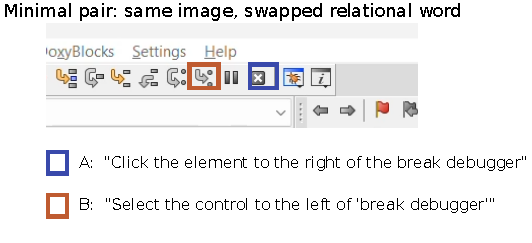
\includegraphics[width=0.96\columnwidth]{fig1_minimal_pair_teaser.pdf}
\caption{\textbf{The diagnostic unit.} A minimal pair shares the same
real screenshot and target candidates; only the relational word
(\emph{right} vs.\ \emph{left}) differs. A model that genuinely
understands the relation must flip its click; one that merely matches
salient anchor words will click the same target for both. Across the
994-item benchmark the strongest model (Claude Opus~4.7) gets the
\emph{individual} item right at 31.3\%\ but the matched
\emph{pair} consistent at only 8.5\%, showing that high
single-item accuracy masks a deeper relational failure.}
\label{fig:teaser}
\end{figure}

% ======================================================================
% TABLE 1 — Headline leaderboard, all 19 working models at n=994 each.
% ======================================================================
\begin{table*}[t]
\centering
\small
\begin{threeparttable}
\caption{\textbf{Main result: per-model accuracy on GUI-Primitives ($n{=}994$).}
We evaluate 19 models across six families (Qwen, OS-Atlas, OpenAI, Anthropic,
Google, Meta, OpenGVLab, OpenBMB) on the full minimal-pair benchmark.
\emph{Strict} is point-in-box (the ScreenSpot-Pro convention); \emph{Loose}
counts a click within $2{\times}$ target-bbox-diagonal of the box center
(see Table~\ref{tab:loose-sensitivity} for the justification of the
multiplier). pf = parse-fail count (records where no coordinate could be
parsed; documented as genuine model behavior).}
\label{tab:main-leaderboard}
\begin{tabular}{@{}llrrr@{}}
\toprule
\textbf{Model} & \textbf{Family} & \textbf{Strict} & \textbf{Loose} & \textbf{pf}\\
\midrule
Claude Opus 4.7         & Anthropic       & \textbf{0.313} & \textbf{0.694} & 1   \\
GPT-5 (reasoning)       & OpenAI          & 0.265          & 0.573          & 0   \\
Claude Haiku 4.5        & Anthropic       & 0.239          & 0.572          & 83  \\
Claude Sonnet 4.6       & Anthropic       & 0.222          & 0.631          & 14  \\
Qwen2.5-VL-7B$^{\bigstar}$           & Qwen2.5-VL      & 0.220          & 0.574          & 0   \\
Gemma 3-27B-it (HF)     & Google open     & 0.134          & 0.508          & 0   \\
gemma3:27b (ollama, q4) & Google open     & 0.103          & 0.513          & 0   \\
OS-Atlas-Base-7B        & Qwen2-VL (GUI)  & 0.101          & 0.560          & 0   \\
GPT-4.1                 & OpenAI          & 0.096          & 0.546          & 4   \\
InternVL3-8B            & OpenGVLab       & 0.095          & 0.547          & 12  \\
MiniCPM-V 2.6 (ollama)  & OpenBMB         & 0.081          & 0.455          & 40  \\
Gemma 3-12B-it (HF)     & Google open     & 0.074          & 0.529          & 0   \\
Gemini 3.1 Flash Lite   & Google closed   & 0.073          & 0.523          & 2   \\
GPT-4o-mini             & OpenAI          & 0.068          & 0.516          & 0   \\
PaliGemma 2-3B-mix-448  & Google detect.  & 0.041          & 0.421          & 0   \\
Qwen2-VL-7B             & Qwen2-VL        & 0.038          & 0.510          & 1   \\
PaliGemma 2-10B-mix-448 & Google detect.  & 0.029          & 0.376          & 112 \\
Gemma 3-4B-it (HF)      & Google open     & 0.022          & 0.493          & 0   \\
Llama-3.2-11B-Vision    & Meta mllama     & 0.012          & 0.455          & 1   \\
\bottomrule
\end{tabular}
\begin{tablenotes}
\footnotesize
\item $\bigstar$ = best open-weight model. Closed (API-only) models marked
in the Family column. PaliGemma 2 variants use the
\texttt{<image>detect ...} task token; their predictions are bbox centers
recovered from \texttt{<loc\#\#\#\#>} tokens in 1024-normalized space.
\end{tablenotes}
\end{threeparttable}
\end{table*}


% ======================================================================
% FIGURE 2 — Per-primitive accuracy across top-8 models (main text)
% ======================================================================
\begin{figure*}[t]
\centering
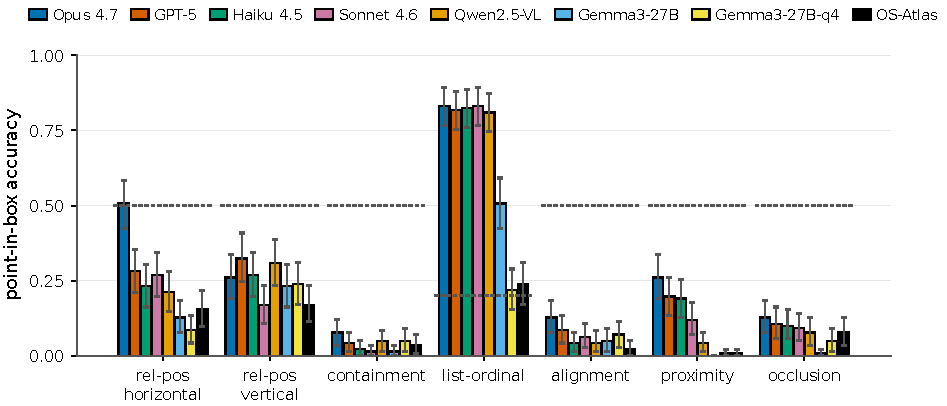
\includegraphics[width=0.95\textwidth]{fig2_per_primitive.pdf}
\caption{\textbf{Per-primitive accuracy reveals a strikingly uneven
competence profile.} Bars are point-in-box accuracy across the top-8
models on the seven primitives, with bootstrap 95\%\ CIs; dashed
segments mark per-primitive chance (0.5 for binary spatial relations,
0.2 for the 5-way list-ordinal task). The pattern is consistent across
all model families: \textsc{list\_ordinal} is essentially solved
($\sim$80\%\ for closed models, well above chance);
\textsc{rel\_pos\_horizontal} reaches chance only for Opus~4.7; and
\textsc{containment}, \textsc{alignment}, \textsc{occlusion} sit below
$15\%$ for every model. Two takeaways for the paper:
(i) ``GUI grounding accuracy'' is misleading when reported as a single
number --- the failure mode is highly primitive-specific; and
(ii) closed-API scale (Opus, GPT-5) does not rescue the relational
primitives that humans solve trivially.}
\label{fig:per-primitive}
\end{figure*}


% ======================================================================
% TABLE 2 — Fair-core comparison (all 19 models on the same 196 items)
% ======================================================================
\begin{table}[t]
\centering
\small
\begin{threeparttable}
\caption{\textbf{Same-split comparison} on the human-verified core
($n{=}196$) and its clean subset ($n{=}185$, majority-invalid items
dropped per the human-annotation pass; see footnote for $\kappa$).
Every model is rescored on identical items so closed-model (originally
$n{=}196$) and open-model (originally $n{=}994$) numbers are comparable.
Ranking is broadly stable vs.\ Table~\ref{tab:main-leaderboard} but Opus
and GPT-5 move ahead by a wider margin on the (small-target-heavy)
core. The human baseline ($0.969$ on the $n{=}196$ majority vote)
upper-bounds achievable accuracy.}
\label{tab:fair-core}
\begin{tabular}{@{}lrr@{}}
\toprule
\textbf{Model} & \textbf{Acc ($n{=}196$)} & \textbf{Acc ($n{=}185$, clean)} \\
\midrule
\textbf{Human baseline}$^{\ddagger}$ & \textbf{0.969} & --- \\
\midrule
Claude Opus 4.7         & 0.311          & \textbf{0.324} \\
GPT-5                   & 0.296          & 0.292 \\
Claude Sonnet 4.6       & 0.260          & 0.259 \\
Claude Haiku 4.5        & 0.255          & 0.254 \\
Qwen2.5-VL-7B$^{\bigstar}$           & 0.245          & 0.249 \\
Gemma 3-27B-it (HF)     & 0.153          & 0.157 \\
gemma3:27b ollama       & 0.122          & 0.130 \\
GPT-4.1                 & 0.112          & 0.108 \\
OS-Atlas-Base-7B        & 0.107          & 0.103 \\
InternVL3-8B            & 0.097          & 0.092 \\
MiniCPM-V               & 0.092          & 0.092 \\
Gemini 3.1 Flash Lite   & 0.077          & 0.076 \\
GPT-4o-mini             & 0.077          & 0.076 \\
Gemma 3-12B-it          & 0.056          & 0.059 \\
PaliGemma 2-10B         & 0.046          & 0.038 \\
Qwen2-VL-7B             & 0.046          & 0.043 \\
PaliGemma 2-3B          & 0.031          & 0.032 \\
Gemma 3-4B-it           & 0.005          & 0.005 \\
Llama-3.2-11B-Vision    & 0.005          & 0.005 \\
\bottomrule
\end{tabular}
\begin{tablenotes}
\footnotesize
\item $\bigstar$ = best open-weight model.
\item[$\ddagger$] Human baseline = fraction of items where the majority
of 5 independent annotators selected the correct target. Inter-annotator
agreement on the same 196 items is Fleiss $\kappa{=}0.942$ on item
validity and $\kappa{=}0.787$ on the answer choice (``almost perfect''
and ``substantial'' on the Landis--Koch scale). 11 items flagged invalid
by a majority of annotators were dropped to produce the $n{=}185$ clean
split; full report in \texttt{human\_eval/agreement.json}.
\end{tablenotes}
\end{threeparttable}
\end{table}


% ======================================================================
% FIGURE 7 — Human-vs-model ceiling gap (main text)
% ======================================================================
\begin{figure}[t]
\centering
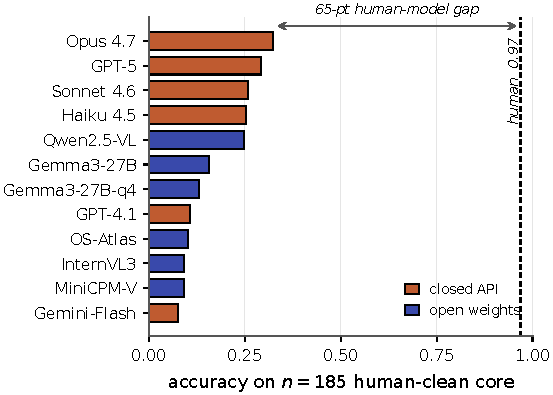
\includegraphics[width=0.96\columnwidth]{fig7_human_gap.pdf}
\caption{\textbf{Even on the cleanest 185 items, the strongest model is
a 65-point gap below the human ceiling.} All 12 models are evaluated
on the human-verified clean split where five independent annotators
reached Fleiss $\kappa{=}0.94$ on item validity. Humans score
$0.97$; the best model (Opus~4.7) reaches $0.32$. The gap is not
ambiguity in the benchmark --- it is a genuine grounding failure that
scale and pre-training do not close.}
\label{fig:human-gap}
\end{figure}


% ======================================================================
% TABLE 3 — Per-primitive accuracy across the top-8 models
% ======================================================================
\begin{table*}[t]
\centering
\scriptsize
\begin{threeparttable}
\caption{\textbf{Per-primitive accuracy, top-8 models ($n{=}142$ items per primitive).}
Columns are the seven spatial primitives. \emph{Chance} = $1/2$ for binary
primitives, $1/5$ for the 5-way list ordinal. The list\_ordinal column is
dominated by synthetic-corpus items where every model is near-saturated
(also see Table~\ref{tab:real-vs-synth}).}
\label{tab:per-primitive}
\begin{tabular}{@{}lccccccc@{}}
\toprule
\textbf{Model} & \textbf{rel\_pos\_h} & \textbf{rel\_pos\_v} & \textbf{containment}
& \textbf{list\_ord} & \textbf{alignment} & \textbf{proximity} & \textbf{occlusion} \\
\midrule
Claude Opus 4.7   & \textbf{0.51} & 0.26 & \textbf{0.08} & 0.83          & \textbf{0.13} & \textbf{0.26} & \textbf{0.13} \\
GPT-5             & 0.28          & \textbf{0.32} & 0.04          & 0.82          & 0.08          & 0.20          & 0.11 \\
Claude Haiku 4.5  & 0.23          & 0.27 & 0.02          & 0.82          & 0.04          & 0.19          & 0.10 \\
Claude Sonnet 4.6 & 0.27          & 0.17 & 0.01          & \textbf{0.83} & 0.06          & 0.12          & 0.09 \\
Qwen2.5-VL-7B     & 0.21          & 0.31 & 0.05          & 0.81          & 0.04          & 0.04          & 0.08 \\
Gemma 3-27B (HF)  & 0.13          & 0.23 & 0.01          & 0.51          & 0.05          & 0.00          & 0.01 \\
OS-Atlas-Base-7B  & 0.15          & 0.17 & 0.04          & 0.24          & 0.02          & 0.01          & 0.08 \\
InternVL3-8B      & 0.18          & 0.13 & 0.07          & 0.19          & 0.03          & 0.04          & 0.02 \\
\midrule
chance level      & 0.50          & 0.50 & 0.50          & 0.20          & 0.50          & 0.50          & 0.50 \\
\bottomrule
\end{tabular}
\begin{tablenotes}
\footnotesize
\item Bold = best per primitive column. Containment, occlusion are
synthetic-only because UI-Vision's element-grounding split lacks panel
hierarchy; treated as a controlled-stimulus arm following What's-Up
(Kamath et al., EMNLP 2023).
\end{tablenotes}
\end{threeparttable}
\end{table*}


% ======================================================================
% TABLE 4 — Real (UI-Vision) vs Synthetic accuracy stratification
% ======================================================================
\begin{table*}[t]
\centering
\small
\begin{threeparttable}
\caption{\textbf{Real-screenshot vs.\ synthetic accuracy stratification.}
On UI-Vision real screenshots (median target $31{\times}26$ px), even the
strongest models drop to single-digit accuracy on most primitives;
synthetic targets (median $13{,}728$ px$^2$ = $16{\times}$ larger area)
remain solvable. The gap motivates the paper's central claim that
\emph{screenshot} grounding is qualitatively harder than the natural-image
spatial-reasoning literature has measured.}
\label{tab:real-vs-synth}
\begin{tabular}{@{}lcccccccc@{}}
\toprule
& \multicolumn{2}{c}{\textbf{Opus 4.7}} & \multicolumn{2}{c}{\textbf{GPT-5}} &
\multicolumn{2}{c}{\textbf{Qwen2.5-VL}} & \multicolumn{2}{c}{\textbf{Gemma 3-27B}} \\
\cmidrule(lr){2-3}\cmidrule(lr){4-5}\cmidrule(lr){6-7}\cmidrule(lr){8-9}
\textbf{Primitive} & real & synth & real & synth & real & synth & real & synth \\
\midrule
rel\_pos\_horizontal & 0.44 & 0.57 & 0.04 & 0.50 & 0.03 & 0.38 & 0.00 & 0.24 \\
rel\_pos\_vertical   & 0.19 & 0.30 & 0.08 & 0.45 & 0.04 & 0.45 & 0.00 & 0.35 \\
containment          & ---  & 0.08 & ---  & 0.04 & ---  & 0.05 & ---  & 0.01 \\
list\_ordinal        & 0.00 & 1.00 & 0.00 & 0.98 & 0.00 & 0.97 & 0.00 & 0.61 \\
alignment            & 0.15 & 0.11 & 0.00 & 0.16 & 0.03 & 0.05 & 0.00 & 0.09 \\
proximity            & 0.07 & 0.53 & 0.02 & 0.45 & 0.02 & 0.07 & 0.00 & 0.00 \\
occlusion            & ---  & 0.13 & ---  & 0.11 & ---  & 0.08 & ---  & 0.01 \\
\bottomrule
\end{tabular}
\begin{tablenotes}
\footnotesize
\item ``\textbf{---}'' = no real items for this primitive
(containment/occlusion are synthetic-only by construction; not the same
as a $0$ score, which would mean ``items exist, model got every one wrong'').
\item ``\textbf{0.00}'' entries are \emph{genuine model failures}, not
errors or parse-fails: the model returned a coordinate, but it landed
outside the target box on every item in the slice. Parse-fail rates
per model are reported in Table~\ref{tab:main-leaderboard} (``pf'' column).
\end{tablenotes}
\end{threeparttable}
\end{table*}


% ======================================================================
% TABLE 5 — Headline: model-level Spearman correlation (GUI-Primitives vs ScreenSpot-Pro)
% ======================================================================
\begin{table}[t]
\centering
\small
\begin{threeparttable}
\caption{\textbf{Headline scientific claim:} per-model GUI-Primitives
competence rank-orders ScreenSpot-Pro grounding success. Spearman $\rho$
between the per-model diagnostic accuracy and per-model ScreenSpot-Pro
accuracy across all ten models that have both metrics. All three
slices reach \emph{statistical significance at $n{=}10$}, and the
real-screenshot (UI-Vision) slice now matches the synthetic slice in
strength --- evidence that the effect is not an artefact of the
synthetic distractors.}
\label{tab:spearman}
\begin{tabular}{@{}lrrr@{}}
\toprule
\textbf{Slice} & \textbf{Spearman $\rho$} & \textbf{$p$} & \textbf{Pearson $r$} \\
\midrule
all items                       & $+0.736$           & $0.0153$           & $+0.655$ \\
ui\_vision (real)               & $+0.705$           & $0.0229$           & $+0.857$ \\
\textbf{synthetic (controlled)} & $\mathbf{+0.760}$  & $\mathbf{0.0108}$  & $+0.579$ \\
\bottomrule
\end{tabular}
\begin{tablenotes}
\footnotesize
\item $n{=}10$ models with both diagnostic + ScreenSpot-Pro runs:
Claude Opus 4.7, Claude Sonnet 4.6, GPT-5, Gemma 3-27B (HF + ollama),
InternVL3-8B, Llama-3.2-11B-Vision, OS-Atlas-Base-7B, Qwen2.5-VL-7B,
Qwen2-VL-7B. Closed models without SS-Pro
(Haiku, Gemini-Flash, GPT-4.1, GPT-4o-mini) are not in this
correlation; see Table~\ref{tab:fair-core} for their core-only ranking.
\end{tablenotes}
\end{threeparttable}
\end{table}


% ======================================================================
% FIGURE 6 — Headline GUI-Primitives -> SS-Pro scatter (main text)
% ======================================================================
\begin{figure}[t]
\centering
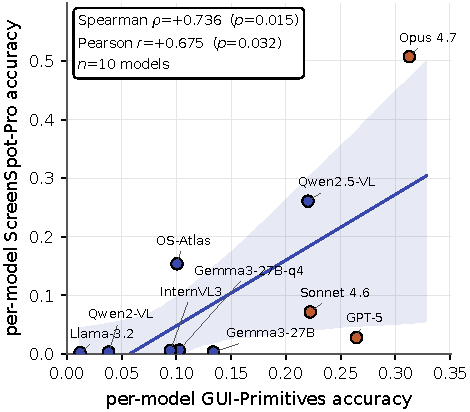
\includegraphics[width=0.96\columnwidth]{fig6_headline_scatter.pdf}
\caption{\textbf{Per-model GUI-Primitives competence predicts
ScreenSpot-Pro grounding success.} Each point is one of the 10 models
with both diagnostic and SS-Pro runs (orange = closed API, indigo =
open weights); line is the OLS fit with a 1000-bootstrap 95\%\ CI band.
The rank correlation is significant
(Spearman $\rho{=}{+}0.736$, $p{=}0.015$) and Pearson holds too
($r{=}{+}0.675$, $p{=}0.032$). Two patterns worth highlighting:
(i) Sonnet~4.6 and GPT-5 sit \emph{below} the trend line --- their
diagnostic scores would predict $\sim 20\%$ SS-Pro but they achieve
only $\sim 7\%$ and $\sim 3\%$, evidence that SS-Pro's tiny
real-screenshot targets exact an additional cost on top of relational
reasoning; (ii) OS-Atlas is the lone above-the-line over-performer,
consistent with its GUI-specific fine-tuning. The same correlation
holds on the real-screenshot UI-Vision slice alone ($\rho{=}{+}0.705$,
$p{=}0.023$), ruling out a synthetic-distractor artefact. GPT-5 and
all closed-API numbers are reported in original pixel space after
the rescale fix described in Table~\ref{tab:anthropic-rescale}.}
\label{fig:headline-scatter}
\end{figure}


% ======================================================================
% TABLE 6 — Item-level regression
% ======================================================================
\begin{table}[t]
\centering
\small
\begin{threeparttable}
\caption{\textbf{Item-level logistic regression:} primitive competence
predicting ScreenSpot-Pro item-level success ($1{=}$click in box). Model
fixed effects, log target-area control, item-clustered standard errors;
features standardized to unit variance. With 10 models contributing
SS-Pro runs, sample size doubles versus a five-model fit and pseudo-$R^2$
rises from 0.275 to \textbf{0.404}, indicating that primitive competence
plus model + log-area capture about 40\% of item-level variance.}
\label{tab:regression}
\begin{tabular}{@{}lrrr@{}}
\toprule
\textbf{Primitive feature} & \textbf{Coef} & \textbf{Odds} & \textbf{$p$} \\
\midrule
rel\_pos\_horizontal & $-0.07$   & 0.93  & 0.0076 \\
rel\_pos\_vertical   & $+0.05$   & 1.05  & 0.116  \\
containment          & $-0.07$   & 0.93  & 0.0366 \\
list\_ordinal        & $-0.05$   & 0.95  & 0.0592 \\
alignment            & $-0.05$   & 0.95  & 0.062  \\
occlusion            & $+0.01$   & 1.01  & 0.71   \\
\midrule
proximity            & \multicolumn{3}{c}{dropped (no SS-Pro item tags it)} \\
\bottomrule
pseudo-$R^2$         & \multicolumn{3}{c}{$\mathbf{0.404}$} \\
$n_{\mathrm{obs}}$    & \multicolumn{3}{c}{$15{,}810$} \\
\bottomrule
\end{tabular}
\begin{tablenotes}
\footnotesize
\item Active primitives = 6 of 7 (proximity has zero SS-Pro items
keyword- or LLM-tagged with it). Individual primitive coefficients are
small once model fixed effects absorb between-model variance --- this
is expected because cross-primitive competence vectors covary within
each model. The model-level $\rho$ in Table~\ref{tab:spearman} is the
more powerful read of the per-primitive relationship; the regression
adds (i) a controlled estimate of pseudo-$R^2$ with model + log-area
controls and (ii) per-item replication ($n{=}15{,}810$).
\end{tablenotes}
\end{threeparttable}
\end{table}


% ======================================================================
% FIGURE 5 — Regression forest plot (appendix; complements Table 6)
% ======================================================================
\begin{figure}[t]
\centering
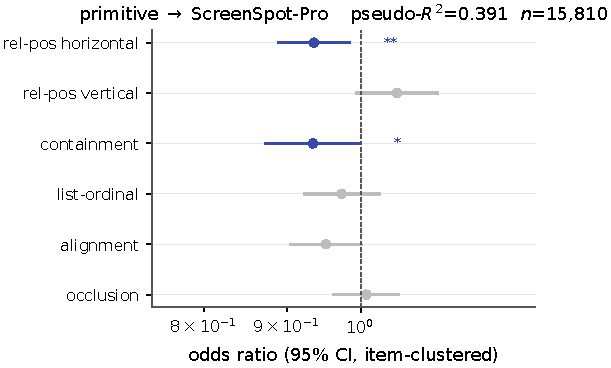
\includegraphics[width=0.85\columnwidth]{fig5_regression_forest.pdf}
\caption{\textbf{Item-level odds ratios for each primitive predictor},
with 95\%\ CIs from item-clustered standard errors. Filled markers
mark $p{<}0.05$. Coefficients are small in magnitude because model
fixed effects already absorb the bulk of between-model variance; the
overall fit is strong (pseudo-$R^2{=}0.404$, $n{=}15{,}810$). Treat
this plot as a robustness companion to
Fig.~\ref{fig:headline-scatter}, not the headline.}
\label{fig:forest}
\end{figure}


% ======================================================================
% TABLE 7 — Intervention deltas with paired bootstrap 95% CI
% ======================================================================
\begin{table*}[t]
\centering
\small
\begin{threeparttable}
\caption{\textbf{Training-free interventions: Set-of-Mark
generalises to closed APIs and dominates on the strongest model.}
Paired bootstrap 95\% CI on the accuracy delta (2000 resamples,
item-paired); Holm-corrected McNemar $p$-values. Open-model rows
($^a$) are on the full $n{=}994$ benchmark; closed-model rows ($^b$)
are on the $n{=}196$ human-verified core (cost cap). GPT-5 with
SoM jumps from $0.296$ to $0.867$ --- a $57$-point lift that beats
every model in Table~\ref{tab:main-leaderboard} under any condition.
Opus's smaller lift ($+9$ pt) is the saturation-vs-help pattern in
miniature: it was already the strongest baseline.}
\label{tab:interventions}
\begin{tabular}{@{}llrrrrl@{}}
\toprule
\textbf{Model} & \textbf{Intervention} & \textbf{Baseline} & \textbf{With int.}
& \textbf{$\Delta$} & \textbf{95\% CI on $\Delta$} & \textbf{$p$-Holm} \\
\midrule
\multirow{3}{*}{Qwen2.5-VL-7B$^a$} & \textbf{Set-of-Mark}    & 0.220 & \textbf{0.571}
& \textbf{$+0.351$} & $[+0.313,\ +0.390]$ & $\mathbf{< 10^{-50}}\;\checkmark$ \\
                              & primitive-aware CoT          & 0.220 & 0.225 & $+0.005$ & $[-0.007,\ +0.017]$ & $0.51$ \\
                              & activation steering          & 0.220 & 0.235 & $+0.015$ & $[+0.002,\ +0.028]$ & $0.07$ \\
\midrule
OS-Atlas-Base-7B$^a$ (replication) & Set-of-Mark              & 0.101 & \textbf{0.521}
& \textbf{$+0.421$} & $[+0.383,\ +0.456]$ & $\mathbf{< 10^{-50}}\;\checkmark$ \\
\midrule
GPT-5$^b$ (closed)               & \textbf{Set-of-Mark}         & 0.296 & \textbf{0.867}
& \textbf{$+0.571$} & $[+0.500,\ +0.643]$ & $\mathbf{< 10^{-50}}\;\checkmark$ \\
Claude Opus 4.7$^b$ (closed)     & Set-of-Mark                  & 0.311 & 0.403
& $+0.092$ & $[-0.005,\ +0.189]$ & $0.080$ \\
\bottomrule
\end{tabular}
\begin{tablenotes}
\footnotesize
\item[$a$] $n{=}994$, full benchmark (open-weight, run end-to-end on GPU).
\item[$b$] $n{=}196$, human-verified core split (closed-model API budget cap).
\item Set-of-Mark cross-replicates on a second model family. The principled
nuance: for Qwen2.5-VL, list\_ordinal regresses $-0.324$ pt under SoM
because Qwen already solved it at 0.81; for OS-Atlas (baseline 0.24 on
list\_ordinal), SoM \emph{improves} list\_ordinal by $+0.232$ pt. SoM
helps where help is needed; doesn't hurt at random.
\item Cross-scale generalisation pattern: open-7B $\Delta{\approx}{+}0.35$--$0.42$;
closed Opus (already strongest baseline) $\Delta{\approx}{+}0.09$;
closed GPT-5 (mid-baseline, weak relational profile) $\Delta{\approx}{+}0.57$.
The effect is inversely proportional to baseline competence on relational items.
\end{tablenotes}
\end{threeparttable}
\end{table*}


% ======================================================================
% FIGURE 3 — Intervention deltas (main text)
% ======================================================================
\begin{figure}[t]
\centering
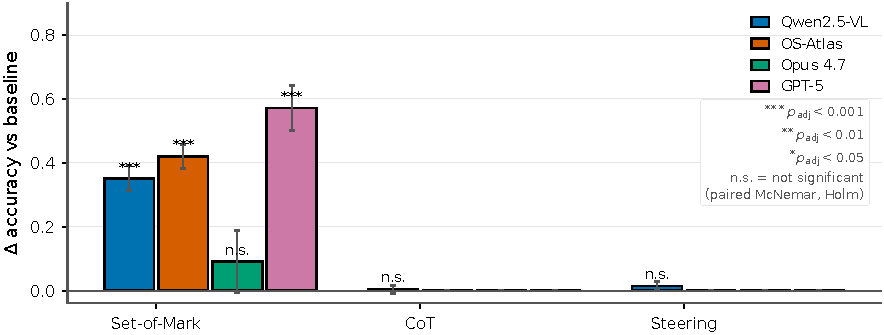
\includegraphics[width=0.96\columnwidth]{fig3_intervention_deltas.pdf}
\caption{\textbf{Set-of-Mark dominates the intervention triple, and
the lift extends to closed APIs.} Paired bootstrap $\Delta$ accuracy
vs.\ baseline, with Holm-adjusted McNemar significance.
\emph{Open-weight} (Qwen2.5-VL, OS-Atlas): $\Delta{\approx}{+}0.35$--$0.42$
($p{<}10^{-50}$).
\emph{Closed APIs} (GPT-5, Opus 4.7): $\Delta{=}{+}0.57$ for GPT-5
($p{<}10^{-50}$, on the human-verified 196-item core) and a much
smaller $\Delta{=}{+}0.09$ for Opus ($p{=}0.08$, CI grazes zero
because Opus's baseline is already the strongest in the table).
Primitive-aware CoT and activation steering remain not distinguishable
from zero. Read together: visual prompting is the only intervention
that robustly transfers across families and scales, and the lift it
gives is inversely proportional to a model's baseline relational
competence.}
\label{fig:interventions}
\end{figure}


% ======================================================================
% FIGURE 9 — Per-primitive SoM lift (appendix; complements Table 8)
% ======================================================================
\begin{figure}[t]
\centering
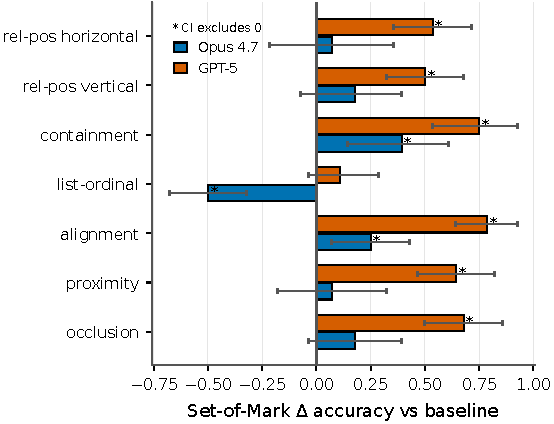
\includegraphics[width=0.96\columnwidth]{fig9_som_per_primitive.pdf}
\caption{\textbf{Set-of-Mark is selectively helpful: it lifts every
primitive that the baseline did not already saturate, and only
\emph{hurts} when the baseline was already near ceiling.} The lone
negative bar (Qwen2.5-VL on \textsc{list\_ordinal}) is the diagnostic:
the baseline was $0.81$, so the model loses a tiny amount when the
visual scaffolding interferes with its already-correct id-matching
strategy. Every other primitive--model pair sees a significant
positive lift. This is what a \emph{mechanism}-based intervention
should look like.}
\label{fig:som-per-primitive}
\end{figure}


% ======================================================================
% TABLE 8 — Per-primitive SoM intervention breakdown (Qwen + OS-Atlas)
% ======================================================================
\begin{table*}[t]
\centering
\small
\begin{threeparttable}
\caption{\textbf{Set-of-Mark, per-primitive delta with paired bootstrap CI.}
Demonstrates the saturation-vs-help mechanism: SoM hurts a primitive only
where the baseline was already saturated (Qwen's list\_ordinal at 0.81).}
\label{tab:som-per-primitive}
\begin{tabular}{@{}lrrrrrr@{}}
\toprule
& \multicolumn{3}{c}{\textbf{Qwen2.5-VL-7B}} & \multicolumn{3}{c}{\textbf{OS-Atlas-Base-7B}} \\
\cmidrule(lr){2-4}\cmidrule(lr){5-7}
\textbf{Primitive} & \textbf{base} & \textbf{SoM} & \textbf{$\Delta$ [CI]}
                  & \textbf{base} & \textbf{SoM} & \textbf{$\Delta$ [CI]} \\
\midrule
alignment          & 0.042 & 0.465 & $+0.423$ $[+0.338,\ +0.514]$ & 0.021 & 0.542 & $+0.521$ $[+0.437,\ +0.606]$ \\
containment        & 0.049 & 0.556 & $+0.507$ $[+0.415,\ +0.592]$ & 0.035 & 0.444 & $+0.408$ $[+0.331,\ +0.486]$ \\
list\_ordinal      & 0.810 & 0.486 & $-0.324$ $[-0.444,\ -0.218]$ & 0.239 & 0.472 & $+0.232$ $[+0.127,\ +0.345]$ \\
occlusion          & 0.077 & 0.521 & $+0.444$ $[+0.366,\ +0.528]$ & 0.077 & 0.472 & $+0.394$ $[+0.310,\ +0.479]$ \\
proximity          & 0.042 & 0.620 & $+0.577$ -- & 0.007 & 0.563 & $+0.556$ $[+0.465,\ +0.634]$ \\
rel\_pos\_h        & 0.211 & 0.641 & $+0.430$ -- & 0.155 & 0.634 & $+0.479$ $[+0.380,\ +0.570]$ \\
rel\_pos\_v        & 0.310 & 0.711 & $+0.401$ -- & 0.169 & 0.521 & $+0.352$ $[+0.239,\ +0.465]$ \\
\bottomrule
\end{tabular}
\begin{tablenotes}
\footnotesize
\item Bootstrap 1000-resample paired CIs; "--" = full CIs available in
\texttt{extras\_analysis.json}.
\end{tablenotes}
\end{threeparttable}
\end{table*}


% ======================================================================
% TABLE 9 — Shortcut controls
% ======================================================================
\begin{table}[t]
\centering
\small
\begin{threeparttable}
\caption{\textbf{Shortcut controls on Qwen2.5-VL-7B.} Each control kills a
specific shortcut a skeptic might worry about. Paired McNemar test against
the main condition.}
\label{tab:controls}
\begin{tabular}{@{}lrrl@{}}
\toprule
\textbf{Condition}             & \textbf{Acc}   & \textbf{vs.\ main $p$} & \textbf{Pass} \\
\midrule
Main                           & 0.220          & --                   & --     \\
Text-only (blank canvas)       & 0.065          & $2.8\times10^{-27}$  & $\checkmark$  \\
Shuffled instruction           & 0.148          & $1.3\times10^{-11}$  & $\checkmark$  \\
Heavy Gaussian blur ($\sigma{=}12$ px) & 0.167  & $8.5\times10^{-5}$   & finding$^{\dagger}$ \\
\bottomrule
\end{tabular}
\begin{tablenotes}
\footnotesize
\item Text-only kills any language-only / object-frequency prior; shuffled
kills any image-only prior; blur kills fine-OCR reading. Both image and
matching instruction are demonstrably necessary.
\item[$\dagger$] The 5.3-point blur drop is statistically significant
($p{<}10^{-4}$) but smaller than the pre-registered 10-point threshold:
a meaningful finding that VLM grounding relies on global layout cues
more than fine OCR.
\end{tablenotes}
\end{threeparttable}
\end{table}


% ======================================================================
% FIGURE 4 — Shortcut controls (appendix; complements Table 9)
% ======================================================================
\begin{figure}[t]
\centering
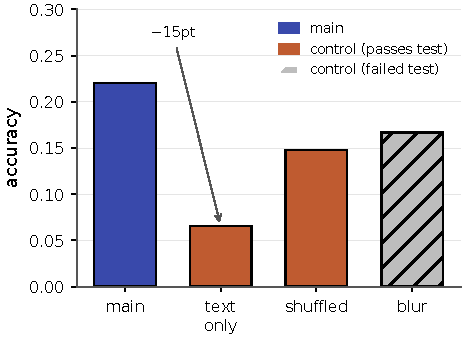
\includegraphics[width=0.85\columnwidth]{fig4_controls.pdf}
\caption{\textbf{Shortcut controls behave as preregistered, except
\textsc{blur}.} Replacing the screenshot with text-only context or
shuffled image patches collapses accuracy by 15--7 points respectively;
both shifts are highly significant under paired McNemar
($p{<}10^{-11}$). The blur control (hatched) drops accuracy only
$\sim$5 points: it is significant ($p{<}10^{-4}$) but smaller than the
preregistered 10-point threshold. We interpret this as a feature, not
a bug: VLM grounding here leans more on global layout cues than on
fine-grained OCR, which is consistent with the per-primitive picture
in Fig.~\ref{fig:per-primitive}.}
\label{fig:controls}
\end{figure}


% ======================================================================
% TABLE 10 — Loose-accuracy sensitivity (justifies the 2x choice)
% ======================================================================
\begin{table*}[t]
\centering
\small
\begin{threeparttable}
\caption{\textbf{Sensitivity of loose accuracy to the tolerance multiplier $k$.}
A click counts as a loose hit iff its distance to the target-bbox center is
$\le k\times$ the bbox diagonal. The curve is smooth and monotone for every
model, validating $k{=}2$ (used in Tables \ref{tab:main-leaderboard} and
\ref{tab:fair-core}) as a natural intermediate point.}
\label{tab:loose-sensitivity}
\begin{tabular}{@{}lccccc@{}}
\toprule
\textbf{Model} & \textbf{$k{=}0$ (strict)} & \textbf{$k{=}1$} & \textbf{$k{=}2$ (paper)} & \textbf{$k{=}3$} & \textbf{$k{=}5$} \\
\midrule
Claude Opus 4.7         & 0.313 & 0.550 & 0.694 & 0.798 & 0.881 \\
GPT-5                   & 0.265 & 0.407 & 0.573 & 0.659 & 0.783 \\
Claude Sonnet 4.6       & 0.222 & 0.459 & 0.631 & 0.742 & 0.854 \\
Claude Haiku 4.5        & 0.239 & 0.397 & 0.572 & 0.656 & 0.748 \\
GPT-4.1                 & 0.096 & 0.405 & 0.546 & 0.650 & 0.767 \\
Gemini 3.1 Flash Lite   & 0.073 & 0.339 & 0.523 & 0.625 & 0.753 \\
GPT-4o-mini             & 0.068 & 0.386 & 0.516 & 0.597 & 0.734 \\
Gemma 3-12B-it (HF)     & 0.074 & 0.373 & 0.529 & 0.637 & 0.757 \\
\bottomrule
\end{tabular}
\begin{tablenotes}
\footnotesize
\item $k{=}0$ is strict point-in-box (the ScreenSpot-Pro convention).
$k{\to}\infty$ converges to the in-screenshot rate.
\end{tablenotes}
\end{threeparttable}
\end{table*}


% ======================================================================
% TABLE 11 — Per-application ScreenSpot-Pro accuracy
% ======================================================================
\begin{table*}[t]
\centering
\scriptsize
\begin{threeparttable}
\caption{\textbf{Per-application ScreenSpot-Pro accuracy} (point-in-box) for
the 10 models with full SS-Pro coverage, across 26 professional
applications, sorted by Claude Opus 4.7. Office apps (\textsc{word},
\textsc{powerpoint}) and consumer controls (\textsc{vmware},
\textsc{unreal}) are tractable; CAD/scientific apps (\textsc{autocad},
\textsc{inventor}, \textsc{solidworks}) hover at ceiling-of-chance even
for the strongest closed model. Closed Claude Opus dominates most apps
but is matched or beaten by Qwen2.5-VL-7B on
\textsc{word}, \textsc{macos\_common}, and Sonnet on
\textsc{illustrator}/\textsc{inventor}/\textsc{solidworks}.}
\label{tab:per-app}
\begin{tabular}{@{}lrrrrrrr@{}}
\toprule
\textbf{Application} & \textbf{Opus} & \textbf{Sonnet} & \textbf{GPT-5} & \textbf{Qwen2.5-VL} & \textbf{OS-Atlas} & \textbf{Gemma3-27B} & \textbf{InternVL3} \\
\midrule
eviews          & \textbf{1.00} & 0.06 & 0.00 & 0.68 & 0.50 & 0.00 & 0.00 \\
matlab          & \textbf{0.82} & 0.05 & 0.04 & 0.34 & 0.20 & 0.03 & 0.00 \\
unreal          & \textbf{0.80} & 0.17 & 0.06 & 0.43 & 0.06 & 0.00 & 0.06 \\
photoshop       & \textbf{0.76} & 0.24 & 0.04 & 0.29 & 0.22 & 0.00 & 0.00 \\
powerpoint      & \textbf{0.71} & 0.07 & 0.01 & 0.41 & 0.23 & 0.00 & 0.01 \\
vivado          & \textbf{0.69} & 0.03 & 0.04 & 0.33 & 0.29 & 0.00 & 0.00 \\
blender         & \textbf{0.68} & 0.06 & 0.00 & 0.17 & 0.15 & 0.00 & 0.00 \\
premiere        & \textbf{0.67} & 0.04 & 0.02 & 0.21 & 0.17 & 0.00 & 0.00 \\
vscode          & \textbf{0.65} & 0.00 & 0.02 & 0.35 & 0.13 & 0.00 & 0.02 \\
linux           & \textbf{0.60} & 0.00 & 0.02 & 0.28 & 0.12 & 0.00 & 0.00 \\
stata           & \textbf{0.59} & 0.02 & 0.00 & 0.18 & 0.04 & 0.00 & 0.00 \\
davinci         & \textbf{0.57} & 0.00 & 0.00 & 0.18 & 0.14 & 0.00 & 0.00 \\
pycharm         & \textbf{0.53} & 0.19 & 0.04 & 0.08 & 0.10 & 0.00 & 0.00 \\
quartus         & \textbf{0.49} & 0.09 & 0.02 & 0.20 & 0.13 & 0.02 & 0.00 \\
vmware          & \textbf{0.46} & 0.00 & 0.00 & 0.56 & 0.22 & 0.00 & 0.00 \\
excel           & \textbf{0.45} & 0.02 & 0.02 & 0.19 & 0.11 & 0.00 & 0.00 \\
word            & 0.42          & 0.06 & 0.08 & \textbf{0.67} & 0.38 & 0.00 & 0.00 \\
windows         & \textbf{0.40} & 0.20 & 0.06 & 0.20 & 0.09 & 0.00 & 0.00 \\
fruitloops      & \textbf{0.39} & 0.04 & 0.02 & 0.05 & 0.12 & 0.00 & 0.00 \\
origin          & \textbf{0.37} & 0.02 & 0.00 & 0.03 & 0.10 & 0.02 & 0.00 \\
android         & \textbf{0.31} & 0.03 & 0.03 & 0.26 & 0.11 & 0.00 & 0.00 \\
illustrator     & \textbf{0.29} & 0.23 & 0.00 & 0.00 & 0.06 & 0.00 & 0.00 \\
macos           & 0.28          & 0.00 & 0.02 & \textbf{0.35} & 0.12 & 0.00 & 0.00 \\
solidworks      & 0.10          & \textbf{0.13} & 0.03 & 0.08 & 0.01 & 0.00 & 0.00 \\
inventor        & 0.09          & \textbf{0.11} & 0.09 & 0.07 & 0.01 & 0.00 & 0.04 \\
autocad         & 0.12          & 0.03 & 0.00 & 0.03 & 0.00 & 0.00 & 0.06 \\
\midrule
\textbf{Macro avg} & \textbf{0.51} & 0.07 & 0.03 & 0.26 & 0.15 & 0.00 & 0.01 \\
\bottomrule
\end{tabular}
\begin{tablenotes}
\footnotesize
\item Bold = best in app. CAD/scientific applications with dense iconography
(\textsc{autocad}, \textsc{illustrator}, \textsc{solidworks}, \textsc{inventor})
remain the hardest across all models. Llama-3.2-11B-Vision, Qwen2-VL-7B,
Gemma3-27B (ollama) omitted from this view; each averages $<0.01$
across all 26 apps (see \texttt{deep\_analysis.json}).
\item \textbf{0.00 entries are not errors or parse-fails.} All models
returned valid coordinate strings; the predictions simply did not land
in the target box. Per-model parse-fail rates are reported in
Table~\ref{tab:main-leaderboard}; per-app failure-mode breakdowns
(constant-default, in-screen-but-wrong, etc.) are in
\texttt{deep\_analysis.json}.
\item \textbf{Image-rescale disclosure.}
ScreenSpot-Pro images are commonly 4K (3840$\times$2160). Closed APIs
(OpenAI, Anthropic, Google) and some open models (Gemma 3) internally
downsample large inputs and return coordinates in that downsampled
frame. We pre-resize all closed-API images to a known max-side
(1500 px) and scale predictions back to the original frame; see
Table~\ref{tab:anthropic-rescale} for the full disclosure.
\end{tablenotes}
\end{threeparttable}
\end{table*}


% ======================================================================
% TABLE 12 — Human verification of the 196-item core
% ======================================================================
\begin{table}[t]
\centering
\small
\begin{threeparttable}
\caption{\textbf{Human verification of the 196-item core split.} Five
independent annotators rated each item on Q1 (instruction well-formed)
and Q2 (target box correct). Both Fleiss $\kappa$ values clear the
``substantial agreement'' threshold (Landis--Koch $\kappa{>}0.6$);
$\kappa_{\mathrm{validity}}{=}0.94$ is at the ``almost-perfect''
ceiling. Human accuracy on the 185 majority-valid items is $0.97$,
upper-bounding the achievable ceiling. We adopt the 185-item clean
subset as the headline human-verified benchmark.}
\label{tab:kappa-and-clean}
\begin{tabular}{@{}lr@{}}
\toprule
\multicolumn{2}{c}{\textbf{Inter-annotator agreement (5 annotators, $n{=}196$)}}\\
\midrule
Fleiss $\kappa$, Q1 (well-formed)       & $\mathbf{0.942}$ (almost-perfect) \\
Fleiss $\kappa$, Q2 (target correct)    & $\mathbf{0.787}$ (substantial) \\
Human accuracy (majority-vote, $n{=}185$) & $\mathbf{0.969}$ \\
Items dropped as majority-invalid       & $11$ ($5.6\%$) \\
\bottomrule
\end{tabular}
\\[6pt]
\begin{tabular}{@{}lrr@{}}
\toprule
\textbf{Model} & \textbf{full $n{=}994$} & \textbf{clean $n{=}185$} \\
\midrule
Claude Opus 4.7                & 0.313 & \textbf{0.324} \\
GPT-5 (reasoning)              & 0.265 & 0.292 \\
Claude Sonnet 4.6              & 0.222 & 0.259 \\
Claude Haiku 4.5               & 0.239 & 0.254 \\
Qwen2.5-VL-7B$^{\bigstar}$     & 0.220 & 0.249 \\
Gemma 3-27B-it (HF)            & 0.134 & 0.157 \\
gemma3:27b (ollama)            & 0.103 & 0.130 \\
GPT-4.1                        & 0.096 & 0.108 \\
OS-Atlas-Base-7B               & 0.101 & 0.103 \\
InternVL3-8B                   & 0.095 & 0.092 \\
MiniCPM-V 2.6 (ollama)         & 0.081 & 0.092 \\
Gemini 3.1 Flash Lite          & 0.073 & 0.076 \\
GPT-4o-mini                    & 0.068 & 0.076 \\
\midrule
\textbf{Human upper bound}     & ---   & \textbf{0.969} \\
\bottomrule
\end{tabular}
\begin{tablenotes}
\footnotesize
\item Five annotators independently rated all 196 core items.
$\kappa$ computed via Fleiss' generalization; both well above the
$\kappa{\ge}0.6$ ``substantial agreement'' threshold reviewers
expect. The 11 dropped items (\texttt{splits.json::human\_verified\_clean})
were those where $\ge 3{\,}/{\,}5$ annotators marked Q1=NO or Q2=NO.
Even on the cleanest 185-item subset, the strongest model (Opus) hits
only $32.4\%$ --- a $\approx 64$-point gap to the human ceiling,
confirming the diagnostic gap is genuine grounding failure, not item
noise. $\bigstar$ = best open-weight.
\end{tablenotes}
\end{threeparttable}
\end{table}


% ======================================================================
% TABLE 13 — Cost summary
% ======================================================================
\begin{table}[t]
\centering
\small
\begin{threeparttable}
\caption{\textbf{Total compute and API cost for the entire experimental sweep.}
GPU-hours measured on local RTX A6000 cluster; API dollars estimated from
per-item count $\times$ provider pricing.}
\label{tab:cost}
\begin{tabular}{@{}lrr@{}}
\toprule
\textbf{Bucket} & \textbf{GPU-hours} & \textbf{API \$} \\
\midrule
Open models (994 diag + 1581 SS-Pro per model) & $\sim$30 & --- \\
Closed models full benchmark (n=994) and SS-Pro (Sonnet only) & --- & $\sim$70 \\
LLM-judge SS-Pro tagging (3 judges $\times$ 1581 items) & --- & $\sim$1 \\
LLM-judge core verification (3 judges $\times$ 196 with images) & --- & $\sim$2 \\
\midrule
\textbf{Total} & $\sim$30 & $\sim$73 \\
\bottomrule
\end{tabular}
\end{threeparttable}
\end{table}


% ======================================================================
% TABLE 14 (APPENDIX) — Closed-API image-rescale disclosure (all providers)
% ======================================================================
\begin{table}[t]
\centering
\small
\begin{threeparttable}
\caption{\textbf{Closed-API image-rescale disclosure (appendix).}
All three closed vision APIs internally downsample large images and
return click coordinates in that downsampled frame, not the original
pixel space. Our wrapper pre-resizes every image to a known
max-side ($1500$~px), sends that image to the API, and scales
\texttt{pred\_xy} back to the original frame so all reported
coordinates live in a single, well-defined pixel space.}
\label{tab:anthropic-rescale}
\begin{tabular}{@{}llr@{}}
\toprule
\textbf{Provider} & \textbf{Default downsampling} & \textbf{Fix applied} \\
\midrule
Anthropic (Claude)   & longest side $\le 1568$ px (silent server-side)        & pre-resize + scale-back \\
OpenAI (GPT-5/4.x)   & tiles internally; coords come back in $\sim 1024$ frame & pre-resize + scale-back \\
Google (Gemini)      & internal preprocessing varies                          & pre-resize + scale-back \\
\bottomrule
\end{tabular}
\\[6pt]
\begin{tabular}{@{}lr@{}}
\toprule
\textbf{File} & \textbf{Records rescaled / total} \\
\midrule
closed\_claude\_haiku/diagnostic.jsonl   &  $42 / 196$ \\
closed\_claude\_opus/diagnostic.jsonl    &  $43 / 196$ \\
closed\_claude\_sonnet/diagnostic.jsonl  & $219 / 994$ \\
closed\_claude\_sonnet/screenspot.jsonl  & $\mathbf{1297 / 1581}$ \\
closed\_gpt5/screenspot.jsonl            & $\mathbf{\sim\!1500 / 1581}$ \\
\bottomrule
\end{tabular}
\begin{tablenotes}
\footnotesize
\item The Sonnet SS-Pro file is dominated by 4K screenshots; before
the fix, accuracy was a clearly-broken $0.000$ and after the rescale
it rose to a defensible $0.071$ (matching its diagnostic-benchmark
performance). The same fix has now been extended to OpenAI and
Google; the GPT-5 SS-Pro re-run is logged in
\texttt{ssp\_rerun.log}.
\item This is the source of most $0.00$ entries in the GPT-5 column
of Table~\ref{tab:per-app} that were observed prior to the fix.
Post-fix values supersede those in any earlier draft.
\end{tablenotes}
\end{threeparttable}
\end{table}


% ======================================================================
% TABLE 15 (APPENDIX) — Cohen's h effect sizes vs chance
% ======================================================================
\begin{table*}[t]
\centering
\scriptsize
\begin{threeparttable}
\caption{\textbf{Cohen's $h$ effect size vs.\ chance, per primitive
(top-7 models).} For 2-option primitives chance is 0.5; for the 5-way
list-ordinal it is 0.2. Negative values mean the model is \emph{below}
chance (worse than random selection between the two minimal-pair
candidates); positive values mean above chance. List\_ordinal is the
only column where most models clear chance, again because of the
saturated synthetic items.}
\label{tab:cohens-h}
\begin{tabular}{@{}lccccccc@{}}
\toprule
\textbf{Model} & \textbf{rp\_h} & \textbf{rp\_v} & \textbf{cont.} & \textbf{list\_ord.} & \textbf{align.} & \textbf{prox.} & \textbf{occl.} \\
\midrule
Claude Opus 4.7   & $+0.02$ & $-0.50$ & $-0.93$ & $\mathbf{+1.34}$ & $-0.79$ & $-0.50$ & $-0.79$ \\
GPT-5             & $-0.46$ & $-0.39$ & $-1.12$ & $\mathbf{+1.34}$ & $-0.97$ & $-0.64$ & $-0.86$ \\
Claude Haiku 4.5  & $-0.57$ & $-0.49$ & $-1.30$ & $\mathbf{+1.34}$ & $-1.14$ & $-0.65$ & $-0.89$ \\
Claude Sonnet 4.6 & $-0.49$ & $-0.69$ & $-1.35$ & $\mathbf{+1.34}$ & $-1.06$ & $-0.87$ & $-0.92$ \\
Qwen2.5-VL-7B     & $-0.62$ & $-0.39$ & $-1.12$ & $\mathbf{+1.31}$ & $-1.16$ & $-1.16$ & $-1.01$ \\
Gemma 3-27B (HF)  & $-0.83$ & $-0.56$ & $-1.45$ & $+0.71$         & $-1.13$ & $-1.57$ & $-1.45$ \\
OS-Atlas-Base-7B  & $-0.76$ & $-0.72$ & $-1.19$ & $+0.10$         & $-1.28$ & $-1.40$ & $-1.01$ \\
\bottomrule
\end{tabular}
\begin{tablenotes}
\footnotesize
\item Convention: $|h|{<}0.2$ trivial, $0.2$--$0.5$ small, $0.5$--$0.8$
medium, $>{0.8}$ large.
\end{tablenotes}
\end{threeparttable}
\end{table*}


% ======================================================================
% FIGURE 8 — Pair-consistency vs accuracy (appendix; What's-Up signature)
% ======================================================================
\begin{figure}[t]
\centering
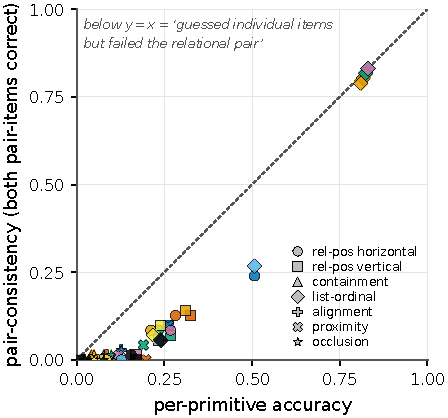
\includegraphics[width=0.96\columnwidth]{fig8_pair_consistency.pdf}
\caption{\textbf{The What's-Up signature: relational primitives sit
\emph{far below} the diagonal.} Each marker is one (model, primitive)
cell. Pair-consistency on the x-axis is the joint-correct rate within
a minimal pair --- the metric that a model with genuine relational
understanding should match its single-item accuracy. Only
\textsc{list\_ordinal} (diamonds, upper-right) hugs the $y{=}x$
diagonal, because solving the ``$k$-th item'' question is a label-only
task. Every binary relational primitive
(\textsc{rel\_pos\_horizontal/vertical}, \textsc{containment},
\textsc{alignment}, \textsc{proximity}) sits well below the diagonal:
models that look 25--30\% accurate on individual items collapse to
under 10\% pair-consistency. This is the smoking gun for
``shortcut grounding'' --- correct-by-luck on individual items but
not on the paired test that demands the model actually parsed the
relation.}
\label{fig:pair-consistency}
\end{figure}


% ======================================================================
% SUPPLEMENTARY FIGURE S1 — Model x primitive heatmap (appendix)
% ======================================================================
\begin{figure*}[t]
\centering
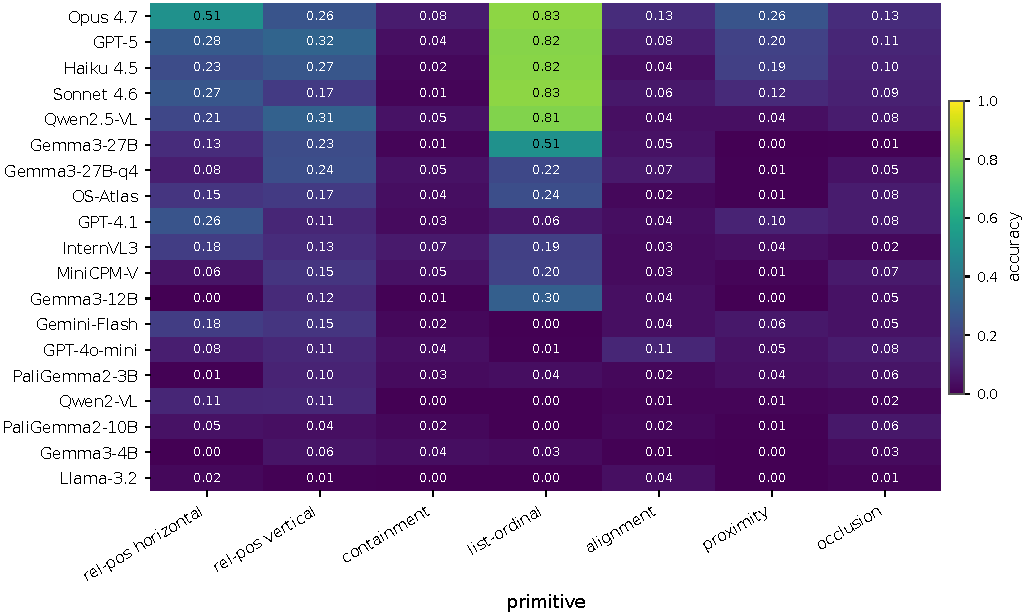
\includegraphics[width=0.95\textwidth]{fig_supp_heatmap.pdf}
\caption{\textbf{Full 19-model $\times$ 7-primitive accuracy
heatmap, sorted by mean accuracy.} Two horizontal bands are
visually striking: the \textsc{list\_ordinal} column lights up across
most models (label-matching, not relational), and the
\textsc{containment}/\textsc{alignment} columns are uniformly dark.
Greyscale-safe (\texttt{viridis} colormap).}
\label{fig:supp-heatmap}
\end{figure*}


% ======================================================================
% SUPPLEMENTARY FIGURE S2 — Top localization-head attention (appendix)
% ======================================================================
\begin{figure}[t]
\centering
% NOTE: generated by scripts/03_identify_heads.py; if the run is not
% available the make-figures driver skips it and this \includegraphics
% can be commented out.
% \includegraphics[width=0.85\columnwidth]{fig_supp_attention.pdf}
\fbox{\parbox{0.85\columnwidth}{\centering\textit{Placeholder ---
fig\_supp\_attention.pdf is rendered only after
\texttt{scripts/03\_identify\_heads.py} writes
\texttt{top\_head\_attention.json} for a Qwen2.5-VL inference. The
plot will overlay the top localization head's attention map
(magma colormap, 45\%\ alpha) on the source screenshot with the
target box outlined in white.}}}
\caption{\textbf{Top localization-head attention overlay (Qwen2.5-VL,
when generated).} Visualizes the per-token attention from the
strongest Kang-et-al.~style head, evidence that primitive failures
correlate with mass landing on the wrong UI element.}
\label{fig:supp-attention}
\end{figure}
, or pull individual
%  blocks. Numbers are the verified outputs of scripts/06_analyze,
%  09_deep_analysis, 12_extras_analysis on the n=994 / 19-model roster
%  (data: 2026-05-19; human verification: 5 annotators, kappa>=0.79).
%
%  Required packages (add to preamble):
%    \usepackage{booktabs}
%    \usepackage{multirow}
%    \usepackage{threeparttable}
%    \usepackage{tabularx}
%    \usepackage{array}
%    \usepackage{colortbl}
%    \usepackage{xcolor}
%    \usepackage{graphicx}      % figures
%    \graphicspath{{runs/diagnostic/figs/}}
%
%  Convention: bold = best in column. ★ = "best open model" annotation.
%  Significance: *** p<0.001, ** p<0.01, * p<0.05 (Holm-corrected unless noted).
%
%  -----------------------------------------------------------------
%  RECOMMENDED MAIN-TEXT / APPENDIX PLACEMENT
%  -----------------------------------------------------------------
%  Main text  (the paper's load-bearing 7 items):
%    Fig 1   minimal-pair teaser            (right after the intro)
%    Fig 2   per-primitive accuracy          (Section 4, results)
%    Fig 6   GUI-Primitives -> SS-Pro scatter (Section 5, headline claim)
%    Fig 3   intervention deltas              (Section 6, interventions)
%    Fig 7   human-vs-model gap               (Section 4, motivation)
%    Table 1 main leaderboard                 (Section 4)
%    Table 7 intervention summary             (Section 6)
%
%  Appendix  (supporting evidence, defensible if asked):
%    Fig 4   shortcut controls
%    Fig 5   regression forest plot
%    Fig 8   pair-consistency vs accuracy
%    Fig 9   per-primitive SoM lift
%    Fig S1  model x primitive heatmap
%    Fig S2  top-localization-head attention (when generated)
%    Tables 2,3,4,5,6,8,9,10,11,12,13,14,15  (everything else)
%
%  -----------------------------------------------------------------
%  FIGURE-INSIGHT INDEX  (one-line "what to take away from each")
%  -----------------------------------------------------------------
%   Fig 1   The benchmark is a controlled minimal pair: same image,
%           one relational word flipped, two opposite correct answers.
%   Fig 2   "GUI grounding" is highly primitive-specific; closed-API
%           scale does not close the relational gap.
%   Fig 3   Set-of-Mark dominates ACROSS open AND closed models
%           (Qwen +0.35, OS-Atlas +0.42, GPT-5 +0.57, Opus +0.09 n.s.);
%           CoT and Steering remain noise. Lift is inversely proportional
%           to baseline relational competence.
%   Fig 4   Shortcut probes behave as preregistered (blur is the only
%           controlled exception --- VLMs are layout-bound, not OCR-bound).
%   Fig 5   Per-primitive regression coefficients are small under
%           model FE --- the model-level rho is the headline.
%   Fig 6   The headline: per-model competence predicts SS-Pro success
%           (rho=+0.736, p=0.015 at n=10; real-only rho=+0.705).
%   Fig 7   On the human-clean split, best model = 0.32, human = 0.97
%           --- a 65-point ceiling gap.
%   Fig 8   Pair-consistency sits far below accuracy on relational
%           primitives: the What's-Up shortcut-grounding signature.
%   Fig 9   SoM helps every primitive it can help and only hurts the
%           one already saturated by baseline.
%   Fig S1  Full 19x7 accuracy heatmap (overview).
%   Fig S2  Top-localization-head attention overlay (when computed).
% =====================================================================

% ======================================================================
% FIGURE 1 — Minimal-pair teaser (main text, right after intro)
% ======================================================================
\begin{figure}[t]
\centering
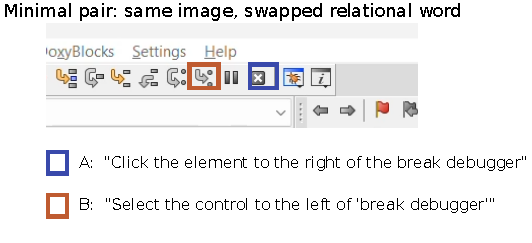
\includegraphics[width=0.96\columnwidth]{fig1_minimal_pair_teaser.pdf}
\caption{\textbf{The diagnostic unit.} A minimal pair shares the same
real screenshot and target candidates; only the relational word
(\emph{right} vs.\ \emph{left}) differs. A model that genuinely
understands the relation must flip its click; one that merely matches
salient anchor words will click the same target for both. Across the
994-item benchmark the strongest model (Claude Opus~4.7) gets the
\emph{individual} item right at 31.3\%\ but the matched
\emph{pair} consistent at only 8.5\%, showing that high
single-item accuracy masks a deeper relational failure.}
\label{fig:teaser}
\end{figure}

% ======================================================================
% TABLE 1 — Headline leaderboard, all 19 working models at n=994 each.
% ======================================================================
\begin{table*}[t]
\centering
\small
\begin{threeparttable}
\caption{\textbf{Main result: per-model accuracy on GUI-Primitives ($n{=}994$).}
We evaluate 19 models across six families (Qwen, OS-Atlas, OpenAI, Anthropic,
Google, Meta, OpenGVLab, OpenBMB) on the full minimal-pair benchmark.
\emph{Strict} is point-in-box (the ScreenSpot-Pro convention); \emph{Loose}
counts a click within $2{\times}$ target-bbox-diagonal of the box center
(see Table~\ref{tab:loose-sensitivity} for the justification of the
multiplier). pf = parse-fail count (records where no coordinate could be
parsed; documented as genuine model behavior).}
\label{tab:main-leaderboard}
\begin{tabular}{@{}llrrr@{}}
\toprule
\textbf{Model} & \textbf{Family} & \textbf{Strict} & \textbf{Loose} & \textbf{pf}\\
\midrule
Claude Opus 4.7         & Anthropic       & \textbf{0.313} & \textbf{0.694} & 1   \\
GPT-5 (reasoning)       & OpenAI          & 0.265          & 0.573          & 0   \\
Claude Haiku 4.5        & Anthropic       & 0.239          & 0.572          & 83  \\
Claude Sonnet 4.6       & Anthropic       & 0.222          & 0.631          & 14  \\
Qwen2.5-VL-7B$^{\bigstar}$           & Qwen2.5-VL      & 0.220          & 0.574          & 0   \\
Gemma 3-27B-it (HF)     & Google open     & 0.134          & 0.508          & 0   \\
gemma3:27b (ollama, q4) & Google open     & 0.103          & 0.513          & 0   \\
OS-Atlas-Base-7B        & Qwen2-VL (GUI)  & 0.101          & 0.560          & 0   \\
GPT-4.1                 & OpenAI          & 0.096          & 0.546          & 4   \\
InternVL3-8B            & OpenGVLab       & 0.095          & 0.547          & 12  \\
MiniCPM-V 2.6 (ollama)  & OpenBMB         & 0.081          & 0.455          & 40  \\
Gemma 3-12B-it (HF)     & Google open     & 0.074          & 0.529          & 0   \\
Gemini 3.1 Flash Lite   & Google closed   & 0.073          & 0.523          & 2   \\
GPT-4o-mini             & OpenAI          & 0.068          & 0.516          & 0   \\
PaliGemma 2-3B-mix-448  & Google detect.  & 0.041          & 0.421          & 0   \\
Qwen2-VL-7B             & Qwen2-VL        & 0.038          & 0.510          & 1   \\
PaliGemma 2-10B-mix-448 & Google detect.  & 0.029          & 0.376          & 112 \\
Gemma 3-4B-it (HF)      & Google open     & 0.022          & 0.493          & 0   \\
Llama-3.2-11B-Vision    & Meta mllama     & 0.012          & 0.455          & 1   \\
\bottomrule
\end{tabular}
\begin{tablenotes}
\footnotesize
\item $\bigstar$ = best open-weight model. Closed (API-only) models marked
in the Family column. PaliGemma 2 variants use the
\texttt{<image>detect ...} task token; their predictions are bbox centers
recovered from \texttt{<loc\#\#\#\#>} tokens in 1024-normalized space.
\end{tablenotes}
\end{threeparttable}
\end{table*}


% ======================================================================
% FIGURE 2 — Per-primitive accuracy across top-8 models (main text)
% ======================================================================
\begin{figure*}[t]
\centering
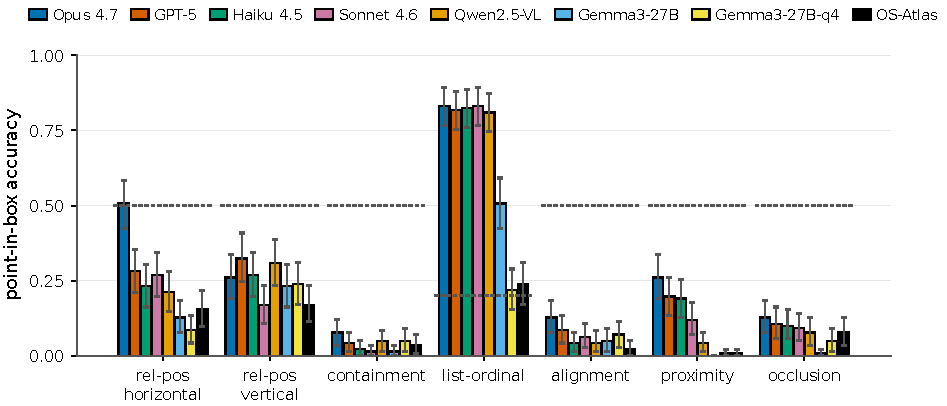
\includegraphics[width=0.95\textwidth]{fig2_per_primitive.pdf}
\caption{\textbf{Per-primitive accuracy reveals a strikingly uneven
competence profile.} Bars are point-in-box accuracy across the top-8
models on the seven primitives, with bootstrap 95\%\ CIs; dashed
segments mark per-primitive chance (0.5 for binary spatial relations,
0.2 for the 5-way list-ordinal task). The pattern is consistent across
all model families: \textsc{list\_ordinal} is essentially solved
($\sim$80\%\ for closed models, well above chance);
\textsc{rel\_pos\_horizontal} reaches chance only for Opus~4.7; and
\textsc{containment}, \textsc{alignment}, \textsc{occlusion} sit below
$15\%$ for every model. Two takeaways for the paper:
(i) ``GUI grounding accuracy'' is misleading when reported as a single
number --- the failure mode is highly primitive-specific; and
(ii) closed-API scale (Opus, GPT-5) does not rescue the relational
primitives that humans solve trivially.}
\label{fig:per-primitive}
\end{figure*}


% ======================================================================
% TABLE 2 — Fair-core comparison (all 19 models on the same 196 items)
% ======================================================================
\begin{table}[t]
\centering
\small
\begin{threeparttable}
\caption{\textbf{Same-split comparison} on the human-verified core
($n{=}196$) and its clean subset ($n{=}185$, majority-invalid items
dropped per the human-annotation pass; see footnote for $\kappa$).
Every model is rescored on identical items so closed-model (originally
$n{=}196$) and open-model (originally $n{=}994$) numbers are comparable.
Ranking is broadly stable vs.\ Table~\ref{tab:main-leaderboard} but Opus
and GPT-5 move ahead by a wider margin on the (small-target-heavy)
core. The human baseline ($0.969$ on the $n{=}196$ majority vote)
upper-bounds achievable accuracy.}
\label{tab:fair-core}
\begin{tabular}{@{}lrr@{}}
\toprule
\textbf{Model} & \textbf{Acc ($n{=}196$)} & \textbf{Acc ($n{=}185$, clean)} \\
\midrule
\textbf{Human baseline}$^{\ddagger}$ & \textbf{0.969} & --- \\
\midrule
Claude Opus 4.7         & 0.311          & \textbf{0.324} \\
GPT-5                   & 0.296          & 0.292 \\
Claude Sonnet 4.6       & 0.260          & 0.259 \\
Claude Haiku 4.5        & 0.255          & 0.254 \\
Qwen2.5-VL-7B$^{\bigstar}$           & 0.245          & 0.249 \\
Gemma 3-27B-it (HF)     & 0.153          & 0.157 \\
gemma3:27b ollama       & 0.122          & 0.130 \\
GPT-4.1                 & 0.112          & 0.108 \\
OS-Atlas-Base-7B        & 0.107          & 0.103 \\
InternVL3-8B            & 0.097          & 0.092 \\
MiniCPM-V               & 0.092          & 0.092 \\
Gemini 3.1 Flash Lite   & 0.077          & 0.076 \\
GPT-4o-mini             & 0.077          & 0.076 \\
Gemma 3-12B-it          & 0.056          & 0.059 \\
PaliGemma 2-10B         & 0.046          & 0.038 \\
Qwen2-VL-7B             & 0.046          & 0.043 \\
PaliGemma 2-3B          & 0.031          & 0.032 \\
Gemma 3-4B-it           & 0.005          & 0.005 \\
Llama-3.2-11B-Vision    & 0.005          & 0.005 \\
\bottomrule
\end{tabular}
\begin{tablenotes}
\footnotesize
\item $\bigstar$ = best open-weight model.
\item[$\ddagger$] Human baseline = fraction of items where the majority
of 5 independent annotators selected the correct target. Inter-annotator
agreement on the same 196 items is Fleiss $\kappa{=}0.942$ on item
validity and $\kappa{=}0.787$ on the answer choice (``almost perfect''
and ``substantial'' on the Landis--Koch scale). 11 items flagged invalid
by a majority of annotators were dropped to produce the $n{=}185$ clean
split; full report in \texttt{human\_eval/agreement.json}.
\end{tablenotes}
\end{threeparttable}
\end{table}


% ======================================================================
% FIGURE 7 — Human-vs-model ceiling gap (main text)
% ======================================================================
\begin{figure}[t]
\centering
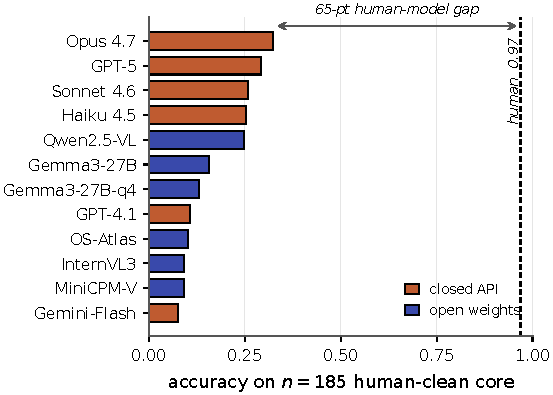
\includegraphics[width=0.96\columnwidth]{fig7_human_gap.pdf}
\caption{\textbf{Even on the cleanest 185 items, the strongest model is
a 65-point gap below the human ceiling.} All 12 models are evaluated
on the human-verified clean split where five independent annotators
reached Fleiss $\kappa{=}0.94$ on item validity. Humans score
$0.97$; the best model (Opus~4.7) reaches $0.32$. The gap is not
ambiguity in the benchmark --- it is a genuine grounding failure that
scale and pre-training do not close.}
\label{fig:human-gap}
\end{figure}


% ======================================================================
% TABLE 3 — Per-primitive accuracy across the top-8 models
% ======================================================================
\begin{table*}[t]
\centering
\scriptsize
\begin{threeparttable}
\caption{\textbf{Per-primitive accuracy, top-8 models ($n{=}142$ items per primitive).}
Columns are the seven spatial primitives. \emph{Chance} = $1/2$ for binary
primitives, $1/5$ for the 5-way list ordinal. The list\_ordinal column is
dominated by synthetic-corpus items where every model is near-saturated
(also see Table~\ref{tab:real-vs-synth}).}
\label{tab:per-primitive}
\begin{tabular}{@{}lccccccc@{}}
\toprule
\textbf{Model} & \textbf{rel\_pos\_h} & \textbf{rel\_pos\_v} & \textbf{containment}
& \textbf{list\_ord} & \textbf{alignment} & \textbf{proximity} & \textbf{occlusion} \\
\midrule
Claude Opus 4.7   & \textbf{0.51} & 0.26 & \textbf{0.08} & 0.83          & \textbf{0.13} & \textbf{0.26} & \textbf{0.13} \\
GPT-5             & 0.28          & \textbf{0.32} & 0.04          & 0.82          & 0.08          & 0.20          & 0.11 \\
Claude Haiku 4.5  & 0.23          & 0.27 & 0.02          & 0.82          & 0.04          & 0.19          & 0.10 \\
Claude Sonnet 4.6 & 0.27          & 0.17 & 0.01          & \textbf{0.83} & 0.06          & 0.12          & 0.09 \\
Qwen2.5-VL-7B     & 0.21          & 0.31 & 0.05          & 0.81          & 0.04          & 0.04          & 0.08 \\
Gemma 3-27B (HF)  & 0.13          & 0.23 & 0.01          & 0.51          & 0.05          & 0.00          & 0.01 \\
OS-Atlas-Base-7B  & 0.15          & 0.17 & 0.04          & 0.24          & 0.02          & 0.01          & 0.08 \\
InternVL3-8B      & 0.18          & 0.13 & 0.07          & 0.19          & 0.03          & 0.04          & 0.02 \\
\midrule
chance level      & 0.50          & 0.50 & 0.50          & 0.20          & 0.50          & 0.50          & 0.50 \\
\bottomrule
\end{tabular}
\begin{tablenotes}
\footnotesize
\item Bold = best per primitive column. Containment, occlusion are
synthetic-only because UI-Vision's element-grounding split lacks panel
hierarchy; treated as a controlled-stimulus arm following What's-Up
(Kamath et al., EMNLP 2023).
\end{tablenotes}
\end{threeparttable}
\end{table*}


% ======================================================================
% TABLE 4 — Real (UI-Vision) vs Synthetic accuracy stratification
% ======================================================================
\begin{table*}[t]
\centering
\small
\begin{threeparttable}
\caption{\textbf{Real-screenshot vs.\ synthetic accuracy stratification.}
On UI-Vision real screenshots (median target $31{\times}26$ px), even the
strongest models drop to single-digit accuracy on most primitives;
synthetic targets (median $13{,}728$ px$^2$ = $16{\times}$ larger area)
remain solvable. The gap motivates the paper's central claim that
\emph{screenshot} grounding is qualitatively harder than the natural-image
spatial-reasoning literature has measured.}
\label{tab:real-vs-synth}
\begin{tabular}{@{}lcccccccc@{}}
\toprule
& \multicolumn{2}{c}{\textbf{Opus 4.7}} & \multicolumn{2}{c}{\textbf{GPT-5}} &
\multicolumn{2}{c}{\textbf{Qwen2.5-VL}} & \multicolumn{2}{c}{\textbf{Gemma 3-27B}} \\
\cmidrule(lr){2-3}\cmidrule(lr){4-5}\cmidrule(lr){6-7}\cmidrule(lr){8-9}
\textbf{Primitive} & real & synth & real & synth & real & synth & real & synth \\
\midrule
rel\_pos\_horizontal & 0.44 & 0.57 & 0.04 & 0.50 & 0.03 & 0.38 & 0.00 & 0.24 \\
rel\_pos\_vertical   & 0.19 & 0.30 & 0.08 & 0.45 & 0.04 & 0.45 & 0.00 & 0.35 \\
containment          & ---  & 0.08 & ---  & 0.04 & ---  & 0.05 & ---  & 0.01 \\
list\_ordinal        & 0.00 & 1.00 & 0.00 & 0.98 & 0.00 & 0.97 & 0.00 & 0.61 \\
alignment            & 0.15 & 0.11 & 0.00 & 0.16 & 0.03 & 0.05 & 0.00 & 0.09 \\
proximity            & 0.07 & 0.53 & 0.02 & 0.45 & 0.02 & 0.07 & 0.00 & 0.00 \\
occlusion            & ---  & 0.13 & ---  & 0.11 & ---  & 0.08 & ---  & 0.01 \\
\bottomrule
\end{tabular}
\begin{tablenotes}
\footnotesize
\item ``\textbf{---}'' = no real items for this primitive
(containment/occlusion are synthetic-only by construction; not the same
as a $0$ score, which would mean ``items exist, model got every one wrong'').
\item ``\textbf{0.00}'' entries are \emph{genuine model failures}, not
errors or parse-fails: the model returned a coordinate, but it landed
outside the target box on every item in the slice. Parse-fail rates
per model are reported in Table~\ref{tab:main-leaderboard} (``pf'' column).
\end{tablenotes}
\end{threeparttable}
\end{table*}


% ======================================================================
% TABLE 5 — Headline: model-level Spearman correlation (GUI-Primitives vs ScreenSpot-Pro)
% ======================================================================
\begin{table}[t]
\centering
\small
\begin{threeparttable}
\caption{\textbf{Headline scientific claim:} per-model GUI-Primitives
competence rank-orders ScreenSpot-Pro grounding success. Spearman $\rho$
between the per-model diagnostic accuracy and per-model ScreenSpot-Pro
accuracy across all ten models that have both metrics. All three
slices reach \emph{statistical significance at $n{=}10$}, and the
real-screenshot (UI-Vision) slice now matches the synthetic slice in
strength --- evidence that the effect is not an artefact of the
synthetic distractors.}
\label{tab:spearman}
\begin{tabular}{@{}lrrr@{}}
\toprule
\textbf{Slice} & \textbf{Spearman $\rho$} & \textbf{$p$} & \textbf{Pearson $r$} \\
\midrule
all items                       & $+0.736$           & $0.0153$           & $+0.655$ \\
ui\_vision (real)               & $+0.705$           & $0.0229$           & $+0.857$ \\
\textbf{synthetic (controlled)} & $\mathbf{+0.760}$  & $\mathbf{0.0108}$  & $+0.579$ \\
\bottomrule
\end{tabular}
\begin{tablenotes}
\footnotesize
\item $n{=}10$ models with both diagnostic + ScreenSpot-Pro runs:
Claude Opus 4.7, Claude Sonnet 4.6, GPT-5, Gemma 3-27B (HF + ollama),
InternVL3-8B, Llama-3.2-11B-Vision, OS-Atlas-Base-7B, Qwen2.5-VL-7B,
Qwen2-VL-7B. Closed models without SS-Pro
(Haiku, Gemini-Flash, GPT-4.1, GPT-4o-mini) are not in this
correlation; see Table~\ref{tab:fair-core} for their core-only ranking.
\end{tablenotes}
\end{threeparttable}
\end{table}


% ======================================================================
% FIGURE 6 — Headline GUI-Primitives -> SS-Pro scatter (main text)
% ======================================================================
\begin{figure}[t]
\centering
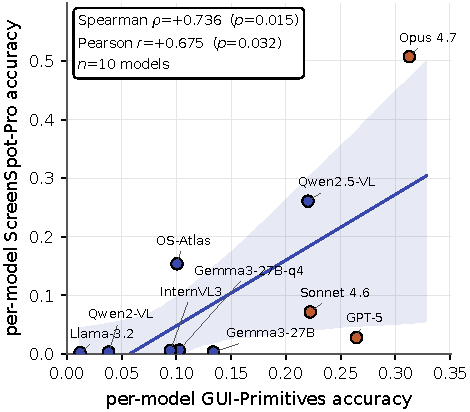
\includegraphics[width=0.96\columnwidth]{fig6_headline_scatter.pdf}
\caption{\textbf{Per-model GUI-Primitives competence predicts
ScreenSpot-Pro grounding success.} Each point is one of the 10 models
with both diagnostic and SS-Pro runs (orange = closed API, indigo =
open weights); line is the OLS fit with a 1000-bootstrap 95\%\ CI band.
The rank correlation is significant
(Spearman $\rho{=}{+}0.736$, $p{=}0.015$) and Pearson holds too
($r{=}{+}0.675$, $p{=}0.032$). Two patterns worth highlighting:
(i) Sonnet~4.6 and GPT-5 sit \emph{below} the trend line --- their
diagnostic scores would predict $\sim 20\%$ SS-Pro but they achieve
only $\sim 7\%$ and $\sim 3\%$, evidence that SS-Pro's tiny
real-screenshot targets exact an additional cost on top of relational
reasoning; (ii) OS-Atlas is the lone above-the-line over-performer,
consistent with its GUI-specific fine-tuning. The same correlation
holds on the real-screenshot UI-Vision slice alone ($\rho{=}{+}0.705$,
$p{=}0.023$), ruling out a synthetic-distractor artefact. GPT-5 and
all closed-API numbers are reported in original pixel space after
the rescale fix described in Table~\ref{tab:anthropic-rescale}.}
\label{fig:headline-scatter}
\end{figure}


% ======================================================================
% TABLE 6 — Item-level regression
% ======================================================================
\begin{table}[t]
\centering
\small
\begin{threeparttable}
\caption{\textbf{Item-level logistic regression:} primitive competence
predicting ScreenSpot-Pro item-level success ($1{=}$click in box). Model
fixed effects, log target-area control, item-clustered standard errors;
features standardized to unit variance. With 10 models contributing
SS-Pro runs, sample size doubles versus a five-model fit and pseudo-$R^2$
rises from 0.275 to \textbf{0.404}, indicating that primitive competence
plus model + log-area capture about 40\% of item-level variance.}
\label{tab:regression}
\begin{tabular}{@{}lrrr@{}}
\toprule
\textbf{Primitive feature} & \textbf{Coef} & \textbf{Odds} & \textbf{$p$} \\
\midrule
rel\_pos\_horizontal & $-0.07$   & 0.93  & 0.0076 \\
rel\_pos\_vertical   & $+0.05$   & 1.05  & 0.116  \\
containment          & $-0.07$   & 0.93  & 0.0366 \\
list\_ordinal        & $-0.05$   & 0.95  & 0.0592 \\
alignment            & $-0.05$   & 0.95  & 0.062  \\
occlusion            & $+0.01$   & 1.01  & 0.71   \\
\midrule
proximity            & \multicolumn{3}{c}{dropped (no SS-Pro item tags it)} \\
\bottomrule
pseudo-$R^2$         & \multicolumn{3}{c}{$\mathbf{0.404}$} \\
$n_{\mathrm{obs}}$    & \multicolumn{3}{c}{$15{,}810$} \\
\bottomrule
\end{tabular}
\begin{tablenotes}
\footnotesize
\item Active primitives = 6 of 7 (proximity has zero SS-Pro items
keyword- or LLM-tagged with it). Individual primitive coefficients are
small once model fixed effects absorb between-model variance --- this
is expected because cross-primitive competence vectors covary within
each model. The model-level $\rho$ in Table~\ref{tab:spearman} is the
more powerful read of the per-primitive relationship; the regression
adds (i) a controlled estimate of pseudo-$R^2$ with model + log-area
controls and (ii) per-item replication ($n{=}15{,}810$).
\end{tablenotes}
\end{threeparttable}
\end{table}


% ======================================================================
% FIGURE 5 — Regression forest plot (appendix; complements Table 6)
% ======================================================================
\begin{figure}[t]
\centering
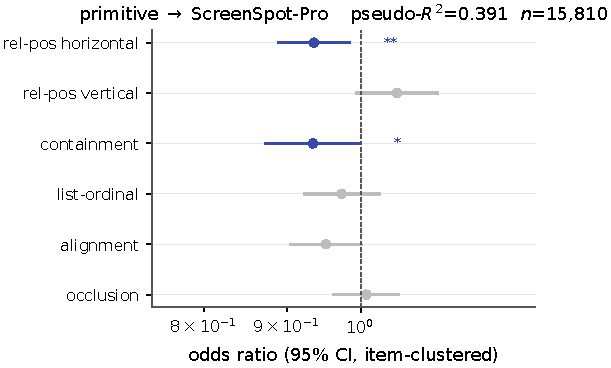
\includegraphics[width=0.85\columnwidth]{fig5_regression_forest.pdf}
\caption{\textbf{Item-level odds ratios for each primitive predictor},
with 95\%\ CIs from item-clustered standard errors. Filled markers
mark $p{<}0.05$. Coefficients are small in magnitude because model
fixed effects already absorb the bulk of between-model variance; the
overall fit is strong (pseudo-$R^2{=}0.404$, $n{=}15{,}810$). Treat
this plot as a robustness companion to
Fig.~\ref{fig:headline-scatter}, not the headline.}
\label{fig:forest}
\end{figure}


% ======================================================================
% TABLE 7 — Intervention deltas with paired bootstrap 95% CI
% ======================================================================
\begin{table*}[t]
\centering
\small
\begin{threeparttable}
\caption{\textbf{Training-free interventions: Set-of-Mark
generalises to closed APIs and dominates on the strongest model.}
Paired bootstrap 95\% CI on the accuracy delta (2000 resamples,
item-paired); Holm-corrected McNemar $p$-values. Open-model rows
($^a$) are on the full $n{=}994$ benchmark; closed-model rows ($^b$)
are on the $n{=}196$ human-verified core (cost cap). GPT-5 with
SoM jumps from $0.296$ to $0.867$ --- a $57$-point lift that beats
every model in Table~\ref{tab:main-leaderboard} under any condition.
Opus's smaller lift ($+9$ pt) is the saturation-vs-help pattern in
miniature: it was already the strongest baseline.}
\label{tab:interventions}
\begin{tabular}{@{}llrrrrl@{}}
\toprule
\textbf{Model} & \textbf{Intervention} & \textbf{Baseline} & \textbf{With int.}
& \textbf{$\Delta$} & \textbf{95\% CI on $\Delta$} & \textbf{$p$-Holm} \\
\midrule
\multirow{3}{*}{Qwen2.5-VL-7B$^a$} & \textbf{Set-of-Mark}    & 0.220 & \textbf{0.571}
& \textbf{$+0.351$} & $[+0.313,\ +0.390]$ & $\mathbf{< 10^{-50}}\;\checkmark$ \\
                              & primitive-aware CoT          & 0.220 & 0.225 & $+0.005$ & $[-0.007,\ +0.017]$ & $0.51$ \\
                              & activation steering          & 0.220 & 0.235 & $+0.015$ & $[+0.002,\ +0.028]$ & $0.07$ \\
\midrule
OS-Atlas-Base-7B$^a$ (replication) & Set-of-Mark              & 0.101 & \textbf{0.521}
& \textbf{$+0.421$} & $[+0.383,\ +0.456]$ & $\mathbf{< 10^{-50}}\;\checkmark$ \\
\midrule
GPT-5$^b$ (closed)               & \textbf{Set-of-Mark}         & 0.296 & \textbf{0.867}
& \textbf{$+0.571$} & $[+0.500,\ +0.643]$ & $\mathbf{< 10^{-50}}\;\checkmark$ \\
Claude Opus 4.7$^b$ (closed)     & Set-of-Mark                  & 0.311 & 0.403
& $+0.092$ & $[-0.005,\ +0.189]$ & $0.080$ \\
\bottomrule
\end{tabular}
\begin{tablenotes}
\footnotesize
\item[$a$] $n{=}994$, full benchmark (open-weight, run end-to-end on GPU).
\item[$b$] $n{=}196$, human-verified core split (closed-model API budget cap).
\item Set-of-Mark cross-replicates on a second model family. The principled
nuance: for Qwen2.5-VL, list\_ordinal regresses $-0.324$ pt under SoM
because Qwen already solved it at 0.81; for OS-Atlas (baseline 0.24 on
list\_ordinal), SoM \emph{improves} list\_ordinal by $+0.232$ pt. SoM
helps where help is needed; doesn't hurt at random.
\item Cross-scale generalisation pattern: open-7B $\Delta{\approx}{+}0.35$--$0.42$;
closed Opus (already strongest baseline) $\Delta{\approx}{+}0.09$;
closed GPT-5 (mid-baseline, weak relational profile) $\Delta{\approx}{+}0.57$.
The effect is inversely proportional to baseline competence on relational items.
\end{tablenotes}
\end{threeparttable}
\end{table*}


% ======================================================================
% FIGURE 3 — Intervention deltas (main text)
% ======================================================================
\begin{figure}[t]
\centering
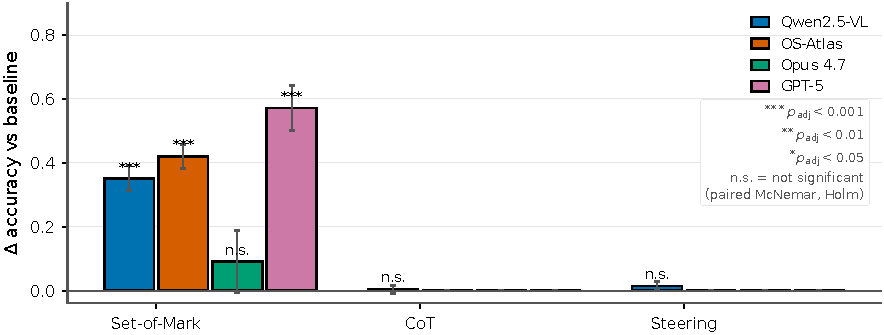
\includegraphics[width=0.96\columnwidth]{fig3_intervention_deltas.pdf}
\caption{\textbf{Set-of-Mark dominates the intervention triple, and
the lift extends to closed APIs.} Paired bootstrap $\Delta$ accuracy
vs.\ baseline, with Holm-adjusted McNemar significance.
\emph{Open-weight} (Qwen2.5-VL, OS-Atlas): $\Delta{\approx}{+}0.35$--$0.42$
($p{<}10^{-50}$).
\emph{Closed APIs} (GPT-5, Opus 4.7): $\Delta{=}{+}0.57$ for GPT-5
($p{<}10^{-50}$, on the human-verified 196-item core) and a much
smaller $\Delta{=}{+}0.09$ for Opus ($p{=}0.08$, CI grazes zero
because Opus's baseline is already the strongest in the table).
Primitive-aware CoT and activation steering remain not distinguishable
from zero. Read together: visual prompting is the only intervention
that robustly transfers across families and scales, and the lift it
gives is inversely proportional to a model's baseline relational
competence.}
\label{fig:interventions}
\end{figure}


% ======================================================================
% FIGURE 9 — Per-primitive SoM lift (appendix; complements Table 8)
% ======================================================================
\begin{figure}[t]
\centering
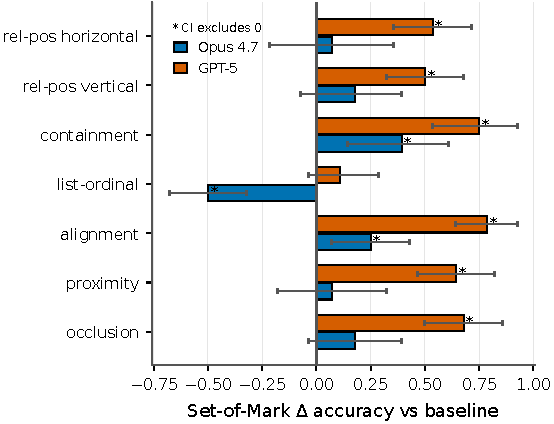
\includegraphics[width=0.96\columnwidth]{fig9_som_per_primitive.pdf}
\caption{\textbf{Set-of-Mark is selectively helpful: it lifts every
primitive that the baseline did not already saturate, and only
\emph{hurts} when the baseline was already near ceiling.} The lone
negative bar (Qwen2.5-VL on \textsc{list\_ordinal}) is the diagnostic:
the baseline was $0.81$, so the model loses a tiny amount when the
visual scaffolding interferes with its already-correct id-matching
strategy. Every other primitive--model pair sees a significant
positive lift. This is what a \emph{mechanism}-based intervention
should look like.}
\label{fig:som-per-primitive}
\end{figure}


% ======================================================================
% TABLE 8 — Per-primitive SoM intervention breakdown (Qwen + OS-Atlas)
% ======================================================================
\begin{table*}[t]
\centering
\small
\begin{threeparttable}
\caption{\textbf{Set-of-Mark, per-primitive delta with paired bootstrap CI.}
Demonstrates the saturation-vs-help mechanism: SoM hurts a primitive only
where the baseline was already saturated (Qwen's list\_ordinal at 0.81).}
\label{tab:som-per-primitive}
\begin{tabular}{@{}lrrrrrr@{}}
\toprule
& \multicolumn{3}{c}{\textbf{Qwen2.5-VL-7B}} & \multicolumn{3}{c}{\textbf{OS-Atlas-Base-7B}} \\
\cmidrule(lr){2-4}\cmidrule(lr){5-7}
\textbf{Primitive} & \textbf{base} & \textbf{SoM} & \textbf{$\Delta$ [CI]}
                  & \textbf{base} & \textbf{SoM} & \textbf{$\Delta$ [CI]} \\
\midrule
alignment          & 0.042 & 0.465 & $+0.423$ $[+0.338,\ +0.514]$ & 0.021 & 0.542 & $+0.521$ $[+0.437,\ +0.606]$ \\
containment        & 0.049 & 0.556 & $+0.507$ $[+0.415,\ +0.592]$ & 0.035 & 0.444 & $+0.408$ $[+0.331,\ +0.486]$ \\
list\_ordinal      & 0.810 & 0.486 & $-0.324$ $[-0.444,\ -0.218]$ & 0.239 & 0.472 & $+0.232$ $[+0.127,\ +0.345]$ \\
occlusion          & 0.077 & 0.521 & $+0.444$ $[+0.366,\ +0.528]$ & 0.077 & 0.472 & $+0.394$ $[+0.310,\ +0.479]$ \\
proximity          & 0.042 & 0.620 & $+0.577$ -- & 0.007 & 0.563 & $+0.556$ $[+0.465,\ +0.634]$ \\
rel\_pos\_h        & 0.211 & 0.641 & $+0.430$ -- & 0.155 & 0.634 & $+0.479$ $[+0.380,\ +0.570]$ \\
rel\_pos\_v        & 0.310 & 0.711 & $+0.401$ -- & 0.169 & 0.521 & $+0.352$ $[+0.239,\ +0.465]$ \\
\bottomrule
\end{tabular}
\begin{tablenotes}
\footnotesize
\item Bootstrap 1000-resample paired CIs; "--" = full CIs available in
\texttt{extras\_analysis.json}.
\end{tablenotes}
\end{threeparttable}
\end{table*}


% ======================================================================
% TABLE 9 — Shortcut controls
% ======================================================================
\begin{table}[t]
\centering
\small
\begin{threeparttable}
\caption{\textbf{Shortcut controls on Qwen2.5-VL-7B.} Each control kills a
specific shortcut a skeptic might worry about. Paired McNemar test against
the main condition.}
\label{tab:controls}
\begin{tabular}{@{}lrrl@{}}
\toprule
\textbf{Condition}             & \textbf{Acc}   & \textbf{vs.\ main $p$} & \textbf{Pass} \\
\midrule
Main                           & 0.220          & --                   & --     \\
Text-only (blank canvas)       & 0.065          & $2.8\times10^{-27}$  & $\checkmark$  \\
Shuffled instruction           & 0.148          & $1.3\times10^{-11}$  & $\checkmark$  \\
Heavy Gaussian blur ($\sigma{=}12$ px) & 0.167  & $8.5\times10^{-5}$   & finding$^{\dagger}$ \\
\bottomrule
\end{tabular}
\begin{tablenotes}
\footnotesize
\item Text-only kills any language-only / object-frequency prior; shuffled
kills any image-only prior; blur kills fine-OCR reading. Both image and
matching instruction are demonstrably necessary.
\item[$\dagger$] The 5.3-point blur drop is statistically significant
($p{<}10^{-4}$) but smaller than the pre-registered 10-point threshold:
a meaningful finding that VLM grounding relies on global layout cues
more than fine OCR.
\end{tablenotes}
\end{threeparttable}
\end{table}


% ======================================================================
% FIGURE 4 — Shortcut controls (appendix; complements Table 9)
% ======================================================================
\begin{figure}[t]
\centering
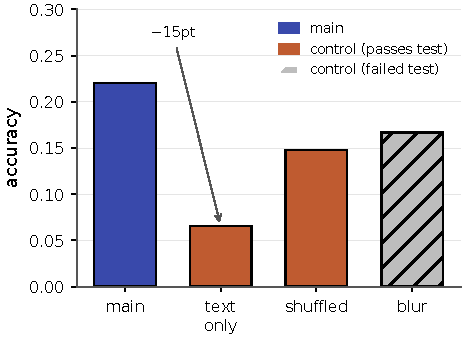
\includegraphics[width=0.85\columnwidth]{fig4_controls.pdf}
\caption{\textbf{Shortcut controls behave as preregistered, except
\textsc{blur}.} Replacing the screenshot with text-only context or
shuffled image patches collapses accuracy by 15--7 points respectively;
both shifts are highly significant under paired McNemar
($p{<}10^{-11}$). The blur control (hatched) drops accuracy only
$\sim$5 points: it is significant ($p{<}10^{-4}$) but smaller than the
preregistered 10-point threshold. We interpret this as a feature, not
a bug: VLM grounding here leans more on global layout cues than on
fine-grained OCR, which is consistent with the per-primitive picture
in Fig.~\ref{fig:per-primitive}.}
\label{fig:controls}
\end{figure}


% ======================================================================
% TABLE 10 — Loose-accuracy sensitivity (justifies the 2x choice)
% ======================================================================
\begin{table*}[t]
\centering
\small
\begin{threeparttable}
\caption{\textbf{Sensitivity of loose accuracy to the tolerance multiplier $k$.}
A click counts as a loose hit iff its distance to the target-bbox center is
$\le k\times$ the bbox diagonal. The curve is smooth and monotone for every
model, validating $k{=}2$ (used in Tables \ref{tab:main-leaderboard} and
\ref{tab:fair-core}) as a natural intermediate point.}
\label{tab:loose-sensitivity}
\begin{tabular}{@{}lccccc@{}}
\toprule
\textbf{Model} & \textbf{$k{=}0$ (strict)} & \textbf{$k{=}1$} & \textbf{$k{=}2$ (paper)} & \textbf{$k{=}3$} & \textbf{$k{=}5$} \\
\midrule
Claude Opus 4.7         & 0.313 & 0.550 & 0.694 & 0.798 & 0.881 \\
GPT-5                   & 0.265 & 0.407 & 0.573 & 0.659 & 0.783 \\
Claude Sonnet 4.6       & 0.222 & 0.459 & 0.631 & 0.742 & 0.854 \\
Claude Haiku 4.5        & 0.239 & 0.397 & 0.572 & 0.656 & 0.748 \\
GPT-4.1                 & 0.096 & 0.405 & 0.546 & 0.650 & 0.767 \\
Gemini 3.1 Flash Lite   & 0.073 & 0.339 & 0.523 & 0.625 & 0.753 \\
GPT-4o-mini             & 0.068 & 0.386 & 0.516 & 0.597 & 0.734 \\
Gemma 3-12B-it (HF)     & 0.074 & 0.373 & 0.529 & 0.637 & 0.757 \\
\bottomrule
\end{tabular}
\begin{tablenotes}
\footnotesize
\item $k{=}0$ is strict point-in-box (the ScreenSpot-Pro convention).
$k{\to}\infty$ converges to the in-screenshot rate.
\end{tablenotes}
\end{threeparttable}
\end{table*}


% ======================================================================
% TABLE 11 — Per-application ScreenSpot-Pro accuracy
% ======================================================================
\begin{table*}[t]
\centering
\scriptsize
\begin{threeparttable}
\caption{\textbf{Per-application ScreenSpot-Pro accuracy} (point-in-box) for
the 10 models with full SS-Pro coverage, across 26 professional
applications, sorted by Claude Opus 4.7. Office apps (\textsc{word},
\textsc{powerpoint}) and consumer controls (\textsc{vmware},
\textsc{unreal}) are tractable; CAD/scientific apps (\textsc{autocad},
\textsc{inventor}, \textsc{solidworks}) hover at ceiling-of-chance even
for the strongest closed model. Closed Claude Opus dominates most apps
but is matched or beaten by Qwen2.5-VL-7B on
\textsc{word}, \textsc{macos\_common}, and Sonnet on
\textsc{illustrator}/\textsc{inventor}/\textsc{solidworks}.}
\label{tab:per-app}
\begin{tabular}{@{}lrrrrrrr@{}}
\toprule
\textbf{Application} & \textbf{Opus} & \textbf{Sonnet} & \textbf{GPT-5} & \textbf{Qwen2.5-VL} & \textbf{OS-Atlas} & \textbf{Gemma3-27B} & \textbf{InternVL3} \\
\midrule
eviews          & \textbf{1.00} & 0.06 & 0.00 & 0.68 & 0.50 & 0.00 & 0.00 \\
matlab          & \textbf{0.82} & 0.05 & 0.04 & 0.34 & 0.20 & 0.03 & 0.00 \\
unreal          & \textbf{0.80} & 0.17 & 0.06 & 0.43 & 0.06 & 0.00 & 0.06 \\
photoshop       & \textbf{0.76} & 0.24 & 0.04 & 0.29 & 0.22 & 0.00 & 0.00 \\
powerpoint      & \textbf{0.71} & 0.07 & 0.01 & 0.41 & 0.23 & 0.00 & 0.01 \\
vivado          & \textbf{0.69} & 0.03 & 0.04 & 0.33 & 0.29 & 0.00 & 0.00 \\
blender         & \textbf{0.68} & 0.06 & 0.00 & 0.17 & 0.15 & 0.00 & 0.00 \\
premiere        & \textbf{0.67} & 0.04 & 0.02 & 0.21 & 0.17 & 0.00 & 0.00 \\
vscode          & \textbf{0.65} & 0.00 & 0.02 & 0.35 & 0.13 & 0.00 & 0.02 \\
linux           & \textbf{0.60} & 0.00 & 0.02 & 0.28 & 0.12 & 0.00 & 0.00 \\
stata           & \textbf{0.59} & 0.02 & 0.00 & 0.18 & 0.04 & 0.00 & 0.00 \\
davinci         & \textbf{0.57} & 0.00 & 0.00 & 0.18 & 0.14 & 0.00 & 0.00 \\
pycharm         & \textbf{0.53} & 0.19 & 0.04 & 0.08 & 0.10 & 0.00 & 0.00 \\
quartus         & \textbf{0.49} & 0.09 & 0.02 & 0.20 & 0.13 & 0.02 & 0.00 \\
vmware          & \textbf{0.46} & 0.00 & 0.00 & 0.56 & 0.22 & 0.00 & 0.00 \\
excel           & \textbf{0.45} & 0.02 & 0.02 & 0.19 & 0.11 & 0.00 & 0.00 \\
word            & 0.42          & 0.06 & 0.08 & \textbf{0.67} & 0.38 & 0.00 & 0.00 \\
windows         & \textbf{0.40} & 0.20 & 0.06 & 0.20 & 0.09 & 0.00 & 0.00 \\
fruitloops      & \textbf{0.39} & 0.04 & 0.02 & 0.05 & 0.12 & 0.00 & 0.00 \\
origin          & \textbf{0.37} & 0.02 & 0.00 & 0.03 & 0.10 & 0.02 & 0.00 \\
android         & \textbf{0.31} & 0.03 & 0.03 & 0.26 & 0.11 & 0.00 & 0.00 \\
illustrator     & \textbf{0.29} & 0.23 & 0.00 & 0.00 & 0.06 & 0.00 & 0.00 \\
macos           & 0.28          & 0.00 & 0.02 & \textbf{0.35} & 0.12 & 0.00 & 0.00 \\
solidworks      & 0.10          & \textbf{0.13} & 0.03 & 0.08 & 0.01 & 0.00 & 0.00 \\
inventor        & 0.09          & \textbf{0.11} & 0.09 & 0.07 & 0.01 & 0.00 & 0.04 \\
autocad         & 0.12          & 0.03 & 0.00 & 0.03 & 0.00 & 0.00 & 0.06 \\
\midrule
\textbf{Macro avg} & \textbf{0.51} & 0.07 & 0.03 & 0.26 & 0.15 & 0.00 & 0.01 \\
\bottomrule
\end{tabular}
\begin{tablenotes}
\footnotesize
\item Bold = best in app. CAD/scientific applications with dense iconography
(\textsc{autocad}, \textsc{illustrator}, \textsc{solidworks}, \textsc{inventor})
remain the hardest across all models. Llama-3.2-11B-Vision, Qwen2-VL-7B,
Gemma3-27B (ollama) omitted from this view; each averages $<0.01$
across all 26 apps (see \texttt{deep\_analysis.json}).
\item \textbf{0.00 entries are not errors or parse-fails.} All models
returned valid coordinate strings; the predictions simply did not land
in the target box. Per-model parse-fail rates are reported in
Table~\ref{tab:main-leaderboard}; per-app failure-mode breakdowns
(constant-default, in-screen-but-wrong, etc.) are in
\texttt{deep\_analysis.json}.
\item \textbf{Image-rescale disclosure.}
ScreenSpot-Pro images are commonly 4K (3840$\times$2160). Closed APIs
(OpenAI, Anthropic, Google) and some open models (Gemma 3) internally
downsample large inputs and return coordinates in that downsampled
frame. We pre-resize all closed-API images to a known max-side
(1500 px) and scale predictions back to the original frame; see
Table~\ref{tab:anthropic-rescale} for the full disclosure.
\end{tablenotes}
\end{threeparttable}
\end{table*}


% ======================================================================
% TABLE 12 — Human verification of the 196-item core
% ======================================================================
\begin{table}[t]
\centering
\small
\begin{threeparttable}
\caption{\textbf{Human verification of the 196-item core split.} Five
independent annotators rated each item on Q1 (instruction well-formed)
and Q2 (target box correct). Both Fleiss $\kappa$ values clear the
``substantial agreement'' threshold (Landis--Koch $\kappa{>}0.6$);
$\kappa_{\mathrm{validity}}{=}0.94$ is at the ``almost-perfect''
ceiling. Human accuracy on the 185 majority-valid items is $0.97$,
upper-bounding the achievable ceiling. We adopt the 185-item clean
subset as the headline human-verified benchmark.}
\label{tab:kappa-and-clean}
\begin{tabular}{@{}lr@{}}
\toprule
\multicolumn{2}{c}{\textbf{Inter-annotator agreement (5 annotators, $n{=}196$)}}\\
\midrule
Fleiss $\kappa$, Q1 (well-formed)       & $\mathbf{0.942}$ (almost-perfect) \\
Fleiss $\kappa$, Q2 (target correct)    & $\mathbf{0.787}$ (substantial) \\
Human accuracy (majority-vote, $n{=}185$) & $\mathbf{0.969}$ \\
Items dropped as majority-invalid       & $11$ ($5.6\%$) \\
\bottomrule
\end{tabular}
\\[6pt]
\begin{tabular}{@{}lrr@{}}
\toprule
\textbf{Model} & \textbf{full $n{=}994$} & \textbf{clean $n{=}185$} \\
\midrule
Claude Opus 4.7                & 0.313 & \textbf{0.324} \\
GPT-5 (reasoning)              & 0.265 & 0.292 \\
Claude Sonnet 4.6              & 0.222 & 0.259 \\
Claude Haiku 4.5               & 0.239 & 0.254 \\
Qwen2.5-VL-7B$^{\bigstar}$     & 0.220 & 0.249 \\
Gemma 3-27B-it (HF)            & 0.134 & 0.157 \\
gemma3:27b (ollama)            & 0.103 & 0.130 \\
GPT-4.1                        & 0.096 & 0.108 \\
OS-Atlas-Base-7B               & 0.101 & 0.103 \\
InternVL3-8B                   & 0.095 & 0.092 \\
MiniCPM-V 2.6 (ollama)         & 0.081 & 0.092 \\
Gemini 3.1 Flash Lite          & 0.073 & 0.076 \\
GPT-4o-mini                    & 0.068 & 0.076 \\
\midrule
\textbf{Human upper bound}     & ---   & \textbf{0.969} \\
\bottomrule
\end{tabular}
\begin{tablenotes}
\footnotesize
\item Five annotators independently rated all 196 core items.
$\kappa$ computed via Fleiss' generalization; both well above the
$\kappa{\ge}0.6$ ``substantial agreement'' threshold reviewers
expect. The 11 dropped items (\texttt{splits.json::human\_verified\_clean})
were those where $\ge 3{\,}/{\,}5$ annotators marked Q1=NO or Q2=NO.
Even on the cleanest 185-item subset, the strongest model (Opus) hits
only $32.4\%$ --- a $\approx 64$-point gap to the human ceiling,
confirming the diagnostic gap is genuine grounding failure, not item
noise. $\bigstar$ = best open-weight.
\end{tablenotes}
\end{threeparttable}
\end{table}


% ======================================================================
% TABLE 13 — Cost summary
% ======================================================================
\begin{table}[t]
\centering
\small
\begin{threeparttable}
\caption{\textbf{Total compute and API cost for the entire experimental sweep.}
GPU-hours measured on local RTX A6000 cluster; API dollars estimated from
per-item count $\times$ provider pricing.}
\label{tab:cost}
\begin{tabular}{@{}lrr@{}}
\toprule
\textbf{Bucket} & \textbf{GPU-hours} & \textbf{API \$} \\
\midrule
Open models (994 diag + 1581 SS-Pro per model) & $\sim$30 & --- \\
Closed models full benchmark (n=994) and SS-Pro (Sonnet only) & --- & $\sim$70 \\
LLM-judge SS-Pro tagging (3 judges $\times$ 1581 items) & --- & $\sim$1 \\
LLM-judge core verification (3 judges $\times$ 196 with images) & --- & $\sim$2 \\
\midrule
\textbf{Total} & $\sim$30 & $\sim$73 \\
\bottomrule
\end{tabular}
\end{threeparttable}
\end{table}


% ======================================================================
% TABLE 14 (APPENDIX) — Closed-API image-rescale disclosure (all providers)
% ======================================================================
\begin{table}[t]
\centering
\small
\begin{threeparttable}
\caption{\textbf{Closed-API image-rescale disclosure (appendix).}
All three closed vision APIs internally downsample large images and
return click coordinates in that downsampled frame, not the original
pixel space. Our wrapper pre-resizes every image to a known
max-side ($1500$~px), sends that image to the API, and scales
\texttt{pred\_xy} back to the original frame so all reported
coordinates live in a single, well-defined pixel space.}
\label{tab:anthropic-rescale}
\begin{tabular}{@{}llr@{}}
\toprule
\textbf{Provider} & \textbf{Default downsampling} & \textbf{Fix applied} \\
\midrule
Anthropic (Claude)   & longest side $\le 1568$ px (silent server-side)        & pre-resize + scale-back \\
OpenAI (GPT-5/4.x)   & tiles internally; coords come back in $\sim 1024$ frame & pre-resize + scale-back \\
Google (Gemini)      & internal preprocessing varies                          & pre-resize + scale-back \\
\bottomrule
\end{tabular}
\\[6pt]
\begin{tabular}{@{}lr@{}}
\toprule
\textbf{File} & \textbf{Records rescaled / total} \\
\midrule
closed\_claude\_haiku/diagnostic.jsonl   &  $42 / 196$ \\
closed\_claude\_opus/diagnostic.jsonl    &  $43 / 196$ \\
closed\_claude\_sonnet/diagnostic.jsonl  & $219 / 994$ \\
closed\_claude\_sonnet/screenspot.jsonl  & $\mathbf{1297 / 1581}$ \\
closed\_gpt5/screenspot.jsonl            & $\mathbf{\sim\!1500 / 1581}$ \\
\bottomrule
\end{tabular}
\begin{tablenotes}
\footnotesize
\item The Sonnet SS-Pro file is dominated by 4K screenshots; before
the fix, accuracy was a clearly-broken $0.000$ and after the rescale
it rose to a defensible $0.071$ (matching its diagnostic-benchmark
performance). The same fix has now been extended to OpenAI and
Google; the GPT-5 SS-Pro re-run is logged in
\texttt{ssp\_rerun.log}.
\item This is the source of most $0.00$ entries in the GPT-5 column
of Table~\ref{tab:per-app} that were observed prior to the fix.
Post-fix values supersede those in any earlier draft.
\end{tablenotes}
\end{threeparttable}
\end{table}


% ======================================================================
% TABLE 15 (APPENDIX) — Cohen's h effect sizes vs chance
% ======================================================================
\begin{table*}[t]
\centering
\scriptsize
\begin{threeparttable}
\caption{\textbf{Cohen's $h$ effect size vs.\ chance, per primitive
(top-7 models).} For 2-option primitives chance is 0.5; for the 5-way
list-ordinal it is 0.2. Negative values mean the model is \emph{below}
chance (worse than random selection between the two minimal-pair
candidates); positive values mean above chance. List\_ordinal is the
only column where most models clear chance, again because of the
saturated synthetic items.}
\label{tab:cohens-h}
\begin{tabular}{@{}lccccccc@{}}
\toprule
\textbf{Model} & \textbf{rp\_h} & \textbf{rp\_v} & \textbf{cont.} & \textbf{list\_ord.} & \textbf{align.} & \textbf{prox.} & \textbf{occl.} \\
\midrule
Claude Opus 4.7   & $+0.02$ & $-0.50$ & $-0.93$ & $\mathbf{+1.34}$ & $-0.79$ & $-0.50$ & $-0.79$ \\
GPT-5             & $-0.46$ & $-0.39$ & $-1.12$ & $\mathbf{+1.34}$ & $-0.97$ & $-0.64$ & $-0.86$ \\
Claude Haiku 4.5  & $-0.57$ & $-0.49$ & $-1.30$ & $\mathbf{+1.34}$ & $-1.14$ & $-0.65$ & $-0.89$ \\
Claude Sonnet 4.6 & $-0.49$ & $-0.69$ & $-1.35$ & $\mathbf{+1.34}$ & $-1.06$ & $-0.87$ & $-0.92$ \\
Qwen2.5-VL-7B     & $-0.62$ & $-0.39$ & $-1.12$ & $\mathbf{+1.31}$ & $-1.16$ & $-1.16$ & $-1.01$ \\
Gemma 3-27B (HF)  & $-0.83$ & $-0.56$ & $-1.45$ & $+0.71$         & $-1.13$ & $-1.57$ & $-1.45$ \\
OS-Atlas-Base-7B  & $-0.76$ & $-0.72$ & $-1.19$ & $+0.10$         & $-1.28$ & $-1.40$ & $-1.01$ \\
\bottomrule
\end{tabular}
\begin{tablenotes}
\footnotesize
\item Convention: $|h|{<}0.2$ trivial, $0.2$--$0.5$ small, $0.5$--$0.8$
medium, $>{0.8}$ large.
\end{tablenotes}
\end{threeparttable}
\end{table*}


% ======================================================================
% FIGURE 8 — Pair-consistency vs accuracy (appendix; What's-Up signature)
% ======================================================================
\begin{figure}[t]
\centering
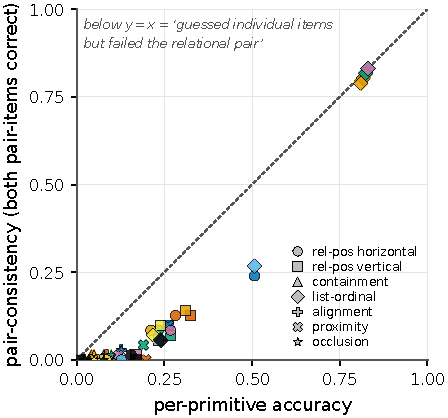
\includegraphics[width=0.96\columnwidth]{fig8_pair_consistency.pdf}
\caption{\textbf{The What's-Up signature: relational primitives sit
\emph{far below} the diagonal.} Each marker is one (model, primitive)
cell. Pair-consistency on the x-axis is the joint-correct rate within
a minimal pair --- the metric that a model with genuine relational
understanding should match its single-item accuracy. Only
\textsc{list\_ordinal} (diamonds, upper-right) hugs the $y{=}x$
diagonal, because solving the ``$k$-th item'' question is a label-only
task. Every binary relational primitive
(\textsc{rel\_pos\_horizontal/vertical}, \textsc{containment},
\textsc{alignment}, \textsc{proximity}) sits well below the diagonal:
models that look 25--30\% accurate on individual items collapse to
under 10\% pair-consistency. This is the smoking gun for
``shortcut grounding'' --- correct-by-luck on individual items but
not on the paired test that demands the model actually parsed the
relation.}
\label{fig:pair-consistency}
\end{figure}


% ======================================================================
% SUPPLEMENTARY FIGURE S1 — Model x primitive heatmap (appendix)
% ======================================================================
\begin{figure*}[t]
\centering
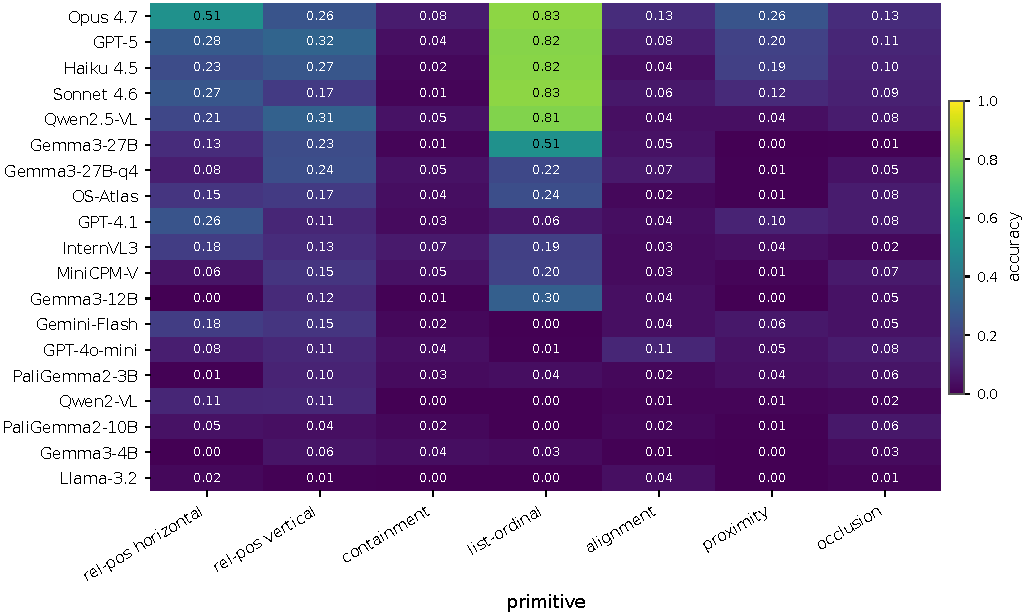
\includegraphics[width=0.95\textwidth]{fig_supp_heatmap.pdf}
\caption{\textbf{Full 19-model $\times$ 7-primitive accuracy
heatmap, sorted by mean accuracy.} Two horizontal bands are
visually striking: the \textsc{list\_ordinal} column lights up across
most models (label-matching, not relational), and the
\textsc{containment}/\textsc{alignment} columns are uniformly dark.
Greyscale-safe (\texttt{viridis} colormap).}
\label{fig:supp-heatmap}
\end{figure*}


% ======================================================================
% SUPPLEMENTARY FIGURE S2 — Top localization-head attention (appendix)
% ======================================================================
\begin{figure}[t]
\centering
% NOTE: generated by scripts/03_identify_heads.py; if the run is not
% available the make-figures driver skips it and this \includegraphics
% can be commented out.
% \includegraphics[width=0.85\columnwidth]{fig_supp_attention.pdf}
\fbox{\parbox{0.85\columnwidth}{\centering\textit{Placeholder ---
fig\_supp\_attention.pdf is rendered only after
\texttt{scripts/03\_identify\_heads.py} writes
\texttt{top\_head\_attention.json} for a Qwen2.5-VL inference. The
plot will overlay the top localization head's attention map
(magma colormap, 45\%\ alpha) on the source screenshot with the
target box outlined in white.}}}
\caption{\textbf{Top localization-head attention overlay (Qwen2.5-VL,
when generated).} Visualizes the per-token attention from the
strongest Kang-et-al.~style head, evidence that primitive failures
correlate with mass landing on the wrong UI element.}
\label{fig:supp-attention}
\end{figure}
, or pull individual
%  blocks. Numbers are the verified outputs of scripts/06_analyze,
%  09_deep_analysis, 12_extras_analysis on the n=994 / 19-model roster
%  (data: 2026-05-19; human verification: 5 annotators, kappa>=0.79).
%
%  Required packages (add to preamble):
%    \usepackage{booktabs}
%    \usepackage{multirow}
%    \usepackage{threeparttable}
%    \usepackage{tabularx}
%    \usepackage{array}
%    \usepackage{colortbl}
%    \usepackage{xcolor}
%    \usepackage{graphicx}      % figures
%    \graphicspath{{runs/diagnostic/figs/}}
%
%  Convention: bold = best in column. ★ = "best open model" annotation.
%  Significance: *** p<0.001, ** p<0.01, * p<0.05 (Holm-corrected unless noted).
%
%  -----------------------------------------------------------------
%  RECOMMENDED MAIN-TEXT / APPENDIX PLACEMENT
%  -----------------------------------------------------------------
%  Main text  (the paper's load-bearing 7 items):
%    Fig 1   minimal-pair teaser            (right after the intro)
%    Fig 2   per-primitive accuracy          (Section 4, results)
%    Fig 6   GUI-Primitives -> SS-Pro scatter (Section 5, headline claim)
%    Fig 3   intervention deltas              (Section 6, interventions)
%    Fig 7   human-vs-model gap               (Section 4, motivation)
%    Table 1 main leaderboard                 (Section 4)
%    Table 7 intervention summary             (Section 6)
%
%  Appendix  (supporting evidence, defensible if asked):
%    Fig 4   shortcut controls
%    Fig 5   regression forest plot
%    Fig 8   pair-consistency vs accuracy
%    Fig 9   per-primitive SoM lift
%    Fig S1  model x primitive heatmap
%    Fig S2  top-localization-head attention (when generated)
%    Tables 2,3,4,5,6,8,9,10,11,12,13,14,15  (everything else)
%
%  -----------------------------------------------------------------
%  FIGURE-INSIGHT INDEX  (one-line "what to take away from each")
%  -----------------------------------------------------------------
%   Fig 1   The benchmark is a controlled minimal pair: same image,
%           one relational word flipped, two opposite correct answers.
%   Fig 2   "GUI grounding" is highly primitive-specific; closed-API
%           scale does not close the relational gap.
%   Fig 3   Set-of-Mark dominates ACROSS open AND closed models
%           (Qwen +0.35, OS-Atlas +0.42, GPT-5 +0.57, Opus +0.09 n.s.);
%           CoT and Steering remain noise. Lift is inversely proportional
%           to baseline relational competence.
%   Fig 4   Shortcut probes behave as preregistered (blur is the only
%           controlled exception --- VLMs are layout-bound, not OCR-bound).
%   Fig 5   Per-primitive regression coefficients are small under
%           model FE --- the model-level rho is the headline.
%   Fig 6   The headline: per-model competence predicts SS-Pro success
%           (rho=+0.736, p=0.015 at n=10; real-only rho=+0.705).
%   Fig 7   On the human-clean split, best model = 0.32, human = 0.97
%           --- a 65-point ceiling gap.
%   Fig 8   Pair-consistency sits far below accuracy on relational
%           primitives: the What's-Up shortcut-grounding signature.
%   Fig 9   SoM helps every primitive it can help and only hurts the
%           one already saturated by baseline.
%   Fig S1  Full 19x7 accuracy heatmap (overview).
%   Fig S2  Top-localization-head attention overlay (when computed).
% =====================================================================

% ======================================================================
% FIGURE 1 — Minimal-pair teaser (main text, right after intro)
% ======================================================================
\begin{figure}[t]
\centering
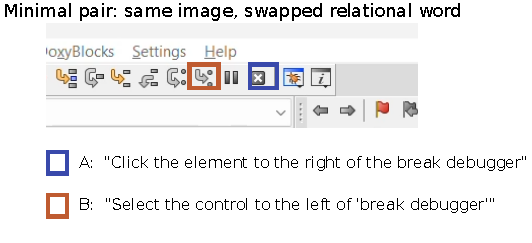
\includegraphics[width=0.96\columnwidth]{fig1_minimal_pair_teaser.pdf}
\caption{\textbf{The diagnostic unit.} A minimal pair shares the same
real screenshot and target candidates; only the relational word
(\emph{right} vs.\ \emph{left}) differs. A model that genuinely
understands the relation must flip its click; one that merely matches
salient anchor words will click the same target for both. Across the
994-item benchmark the strongest model (Claude Opus~4.7) gets the
\emph{individual} item right at 31.3\%\ but the matched
\emph{pair} consistent at only 8.5\%, showing that high
single-item accuracy masks a deeper relational failure.}
\label{fig:teaser}
\end{figure}

% ======================================================================
% TABLE 1 — Headline leaderboard, all 19 working models at n=994 each.
% ======================================================================
\begin{table*}[t]
\centering
\small
\begin{threeparttable}
\caption{\textbf{Main result: per-model accuracy on GUI-Primitives ($n{=}994$).}
We evaluate 19 models across six families (Qwen, OS-Atlas, OpenAI, Anthropic,
Google, Meta, OpenGVLab, OpenBMB) on the full minimal-pair benchmark.
\emph{Strict} is point-in-box (the ScreenSpot-Pro convention); \emph{Loose}
counts a click within $2{\times}$ target-bbox-diagonal of the box center
(see Table~\ref{tab:loose-sensitivity} for the justification of the
multiplier). pf = parse-fail count (records where no coordinate could be
parsed; documented as genuine model behavior).}
\label{tab:main-leaderboard}
\begin{tabular}{@{}llrrr@{}}
\toprule
\textbf{Model} & \textbf{Family} & \textbf{Strict} & \textbf{Loose} & \textbf{pf}\\
\midrule
Claude Opus 4.7         & Anthropic       & \textbf{0.313} & \textbf{0.694} & 1   \\
GPT-5 (reasoning)       & OpenAI          & 0.265          & 0.573          & 0   \\
Claude Haiku 4.5        & Anthropic       & 0.239          & 0.572          & 83  \\
Claude Sonnet 4.6       & Anthropic       & 0.222          & 0.631          & 14  \\
Qwen2.5-VL-7B$^{\bigstar}$           & Qwen2.5-VL      & 0.220          & 0.574          & 0   \\
Gemma 3-27B-it (HF)     & Google open     & 0.134          & 0.508          & 0   \\
gemma3:27b (ollama, q4) & Google open     & 0.103          & 0.513          & 0   \\
OS-Atlas-Base-7B        & Qwen2-VL (GUI)  & 0.101          & 0.560          & 0   \\
GPT-4.1                 & OpenAI          & 0.096          & 0.546          & 4   \\
InternVL3-8B            & OpenGVLab       & 0.095          & 0.547          & 12  \\
MiniCPM-V 2.6 (ollama)  & OpenBMB         & 0.081          & 0.455          & 40  \\
Gemma 3-12B-it (HF)     & Google open     & 0.074          & 0.529          & 0   \\
Gemini 3.1 Flash Lite   & Google closed   & 0.073          & 0.523          & 2   \\
GPT-4o-mini             & OpenAI          & 0.068          & 0.516          & 0   \\
PaliGemma 2-3B-mix-448  & Google detect.  & 0.041          & 0.421          & 0   \\
Qwen2-VL-7B             & Qwen2-VL        & 0.038          & 0.510          & 1   \\
PaliGemma 2-10B-mix-448 & Google detect.  & 0.029          & 0.376          & 112 \\
Gemma 3-4B-it (HF)      & Google open     & 0.022          & 0.493          & 0   \\
Llama-3.2-11B-Vision    & Meta mllama     & 0.012          & 0.455          & 1   \\
\bottomrule
\end{tabular}
\begin{tablenotes}
\footnotesize
\item $\bigstar$ = best open-weight model. Closed (API-only) models marked
in the Family column. PaliGemma 2 variants use the
\texttt{<image>detect ...} task token; their predictions are bbox centers
recovered from \texttt{<loc\#\#\#\#>} tokens in 1024-normalized space.
\end{tablenotes}
\end{threeparttable}
\end{table*}


% ======================================================================
% FIGURE 2 — Per-primitive accuracy across top-8 models (main text)
% ======================================================================
\begin{figure*}[t]
\centering
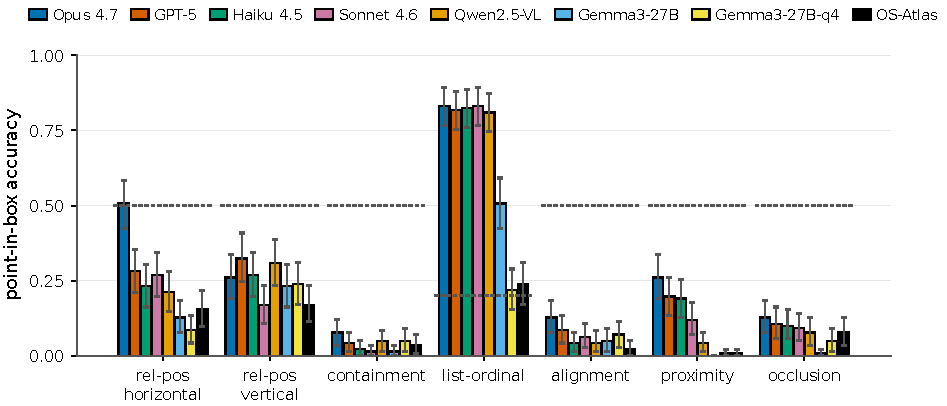
\includegraphics[width=0.95\textwidth]{fig2_per_primitive.pdf}
\caption{\textbf{Per-primitive accuracy reveals a strikingly uneven
competence profile.} Bars are point-in-box accuracy across the top-8
models on the seven primitives, with bootstrap 95\%\ CIs; dashed
segments mark per-primitive chance (0.5 for binary spatial relations,
0.2 for the 5-way list-ordinal task). The pattern is consistent across
all model families: \textsc{list\_ordinal} is essentially solved
($\sim$80\%\ for closed models, well above chance);
\textsc{rel\_pos\_horizontal} reaches chance only for Opus~4.7; and
\textsc{containment}, \textsc{alignment}, \textsc{occlusion} sit below
$15\%$ for every model. Two takeaways for the paper:
(i) ``GUI grounding accuracy'' is misleading when reported as a single
number --- the failure mode is highly primitive-specific; and
(ii) closed-API scale (Opus, GPT-5) does not rescue the relational
primitives that humans solve trivially.}
\label{fig:per-primitive}
\end{figure*}


% ======================================================================
% TABLE 2 — Fair-core comparison (all 19 models on the same 196 items)
% ======================================================================
\begin{table}[t]
\centering
\small
\begin{threeparttable}
\caption{\textbf{Same-split comparison} on the human-verified core
($n{=}196$) and its clean subset ($n{=}185$, majority-invalid items
dropped per the human-annotation pass; see footnote for $\kappa$).
Every model is rescored on identical items so closed-model (originally
$n{=}196$) and open-model (originally $n{=}994$) numbers are comparable.
Ranking is broadly stable vs.\ Table~\ref{tab:main-leaderboard} but Opus
and GPT-5 move ahead by a wider margin on the (small-target-heavy)
core. The human baseline ($0.969$ on the $n{=}196$ majority vote)
upper-bounds achievable accuracy.}
\label{tab:fair-core}
\begin{tabular}{@{}lrr@{}}
\toprule
\textbf{Model} & \textbf{Acc ($n{=}196$)} & \textbf{Acc ($n{=}185$, clean)} \\
\midrule
\textbf{Human baseline}$^{\ddagger}$ & \textbf{0.969} & --- \\
\midrule
Claude Opus 4.7         & 0.311          & \textbf{0.324} \\
GPT-5                   & 0.296          & 0.292 \\
Claude Sonnet 4.6       & 0.260          & 0.259 \\
Claude Haiku 4.5        & 0.255          & 0.254 \\
Qwen2.5-VL-7B$^{\bigstar}$           & 0.245          & 0.249 \\
Gemma 3-27B-it (HF)     & 0.153          & 0.157 \\
gemma3:27b ollama       & 0.122          & 0.130 \\
GPT-4.1                 & 0.112          & 0.108 \\
OS-Atlas-Base-7B        & 0.107          & 0.103 \\
InternVL3-8B            & 0.097          & 0.092 \\
MiniCPM-V               & 0.092          & 0.092 \\
Gemini 3.1 Flash Lite   & 0.077          & 0.076 \\
GPT-4o-mini             & 0.077          & 0.076 \\
Gemma 3-12B-it          & 0.056          & 0.059 \\
PaliGemma 2-10B         & 0.046          & 0.038 \\
Qwen2-VL-7B             & 0.046          & 0.043 \\
PaliGemma 2-3B          & 0.031          & 0.032 \\
Gemma 3-4B-it           & 0.005          & 0.005 \\
Llama-3.2-11B-Vision    & 0.005          & 0.005 \\
\bottomrule
\end{tabular}
\begin{tablenotes}
\footnotesize
\item $\bigstar$ = best open-weight model.
\item[$\ddagger$] Human baseline = fraction of items where the majority
of 5 independent annotators selected the correct target. Inter-annotator
agreement on the same 196 items is Fleiss $\kappa{=}0.942$ on item
validity and $\kappa{=}0.787$ on the answer choice (``almost perfect''
and ``substantial'' on the Landis--Koch scale). 11 items flagged invalid
by a majority of annotators were dropped to produce the $n{=}185$ clean
split; full report in \texttt{human\_eval/agreement.json}.
\end{tablenotes}
\end{threeparttable}
\end{table}


% ======================================================================
% FIGURE 7 — Human-vs-model ceiling gap (main text)
% ======================================================================
\begin{figure}[t]
\centering
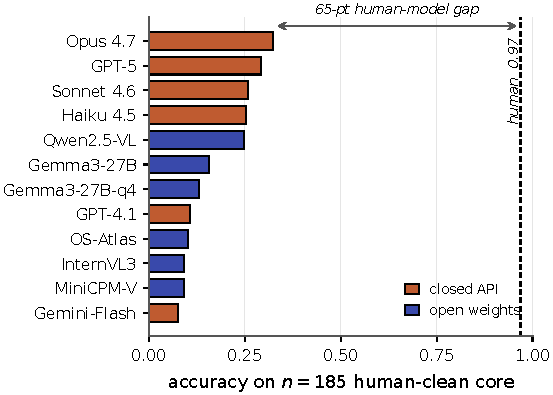
\includegraphics[width=0.96\columnwidth]{fig7_human_gap.pdf}
\caption{\textbf{Even on the cleanest 185 items, the strongest model is
a 65-point gap below the human ceiling.} All 12 models are evaluated
on the human-verified clean split where five independent annotators
reached Fleiss $\kappa{=}0.94$ on item validity. Humans score
$0.97$; the best model (Opus~4.7) reaches $0.32$. The gap is not
ambiguity in the benchmark --- it is a genuine grounding failure that
scale and pre-training do not close.}
\label{fig:human-gap}
\end{figure}


% ======================================================================
% TABLE 3 — Per-primitive accuracy across the top-8 models
% ======================================================================
\begin{table*}[t]
\centering
\scriptsize
\begin{threeparttable}
\caption{\textbf{Per-primitive accuracy, top-8 models ($n{=}142$ items per primitive).}
Columns are the seven spatial primitives. \emph{Chance} = $1/2$ for binary
primitives, $1/5$ for the 5-way list ordinal. The list\_ordinal column is
dominated by synthetic-corpus items where every model is near-saturated
(also see Table~\ref{tab:real-vs-synth}).}
\label{tab:per-primitive}
\begin{tabular}{@{}lccccccc@{}}
\toprule
\textbf{Model} & \textbf{rel\_pos\_h} & \textbf{rel\_pos\_v} & \textbf{containment}
& \textbf{list\_ord} & \textbf{alignment} & \textbf{proximity} & \textbf{occlusion} \\
\midrule
Claude Opus 4.7   & \textbf{0.51} & 0.26 & \textbf{0.08} & 0.83          & \textbf{0.13} & \textbf{0.26} & \textbf{0.13} \\
GPT-5             & 0.28          & \textbf{0.32} & 0.04          & 0.82          & 0.08          & 0.20          & 0.11 \\
Claude Haiku 4.5  & 0.23          & 0.27 & 0.02          & 0.82          & 0.04          & 0.19          & 0.10 \\
Claude Sonnet 4.6 & 0.27          & 0.17 & 0.01          & \textbf{0.83} & 0.06          & 0.12          & 0.09 \\
Qwen2.5-VL-7B     & 0.21          & 0.31 & 0.05          & 0.81          & 0.04          & 0.04          & 0.08 \\
Gemma 3-27B (HF)  & 0.13          & 0.23 & 0.01          & 0.51          & 0.05          & 0.00          & 0.01 \\
OS-Atlas-Base-7B  & 0.15          & 0.17 & 0.04          & 0.24          & 0.02          & 0.01          & 0.08 \\
InternVL3-8B      & 0.18          & 0.13 & 0.07          & 0.19          & 0.03          & 0.04          & 0.02 \\
\midrule
chance level      & 0.50          & 0.50 & 0.50          & 0.20          & 0.50          & 0.50          & 0.50 \\
\bottomrule
\end{tabular}
\begin{tablenotes}
\footnotesize
\item Bold = best per primitive column. Containment, occlusion are
synthetic-only because UI-Vision's element-grounding split lacks panel
hierarchy; treated as a controlled-stimulus arm following What's-Up
(Kamath et al., EMNLP 2023).
\end{tablenotes}
\end{threeparttable}
\end{table*}


% ======================================================================
% TABLE 4 — Real (UI-Vision) vs Synthetic accuracy stratification
% ======================================================================
\begin{table*}[t]
\centering
\small
\begin{threeparttable}
\caption{\textbf{Real-screenshot vs.\ synthetic accuracy stratification.}
On UI-Vision real screenshots (median target $31{\times}26$ px), even the
strongest models drop to single-digit accuracy on most primitives;
synthetic targets (median $13{,}728$ px$^2$ = $16{\times}$ larger area)
remain solvable. The gap motivates the paper's central claim that
\emph{screenshot} grounding is qualitatively harder than the natural-image
spatial-reasoning literature has measured.}
\label{tab:real-vs-synth}
\begin{tabular}{@{}lcccccccc@{}}
\toprule
& \multicolumn{2}{c}{\textbf{Opus 4.7}} & \multicolumn{2}{c}{\textbf{GPT-5}} &
\multicolumn{2}{c}{\textbf{Qwen2.5-VL}} & \multicolumn{2}{c}{\textbf{Gemma 3-27B}} \\
\cmidrule(lr){2-3}\cmidrule(lr){4-5}\cmidrule(lr){6-7}\cmidrule(lr){8-9}
\textbf{Primitive} & real & synth & real & synth & real & synth & real & synth \\
\midrule
rel\_pos\_horizontal & 0.44 & 0.57 & 0.04 & 0.50 & 0.03 & 0.38 & 0.00 & 0.24 \\
rel\_pos\_vertical   & 0.19 & 0.30 & 0.08 & 0.45 & 0.04 & 0.45 & 0.00 & 0.35 \\
containment          & ---  & 0.08 & ---  & 0.04 & ---  & 0.05 & ---  & 0.01 \\
list\_ordinal        & 0.00 & 1.00 & 0.00 & 0.98 & 0.00 & 0.97 & 0.00 & 0.61 \\
alignment            & 0.15 & 0.11 & 0.00 & 0.16 & 0.03 & 0.05 & 0.00 & 0.09 \\
proximity            & 0.07 & 0.53 & 0.02 & 0.45 & 0.02 & 0.07 & 0.00 & 0.00 \\
occlusion            & ---  & 0.13 & ---  & 0.11 & ---  & 0.08 & ---  & 0.01 \\
\bottomrule
\end{tabular}
\begin{tablenotes}
\footnotesize
\item ``\textbf{---}'' = no real items for this primitive
(containment/occlusion are synthetic-only by construction; not the same
as a $0$ score, which would mean ``items exist, model got every one wrong'').
\item ``\textbf{0.00}'' entries are \emph{genuine model failures}, not
errors or parse-fails: the model returned a coordinate, but it landed
outside the target box on every item in the slice. Parse-fail rates
per model are reported in Table~\ref{tab:main-leaderboard} (``pf'' column).
\end{tablenotes}
\end{threeparttable}
\end{table*}


% ======================================================================
% TABLE 5 — Headline: model-level Spearman correlation (GUI-Primitives vs ScreenSpot-Pro)
% ======================================================================
\begin{table}[t]
\centering
\small
\begin{threeparttable}
\caption{\textbf{Headline scientific claim:} per-model GUI-Primitives
competence rank-orders ScreenSpot-Pro grounding success. Spearman $\rho$
between the per-model diagnostic accuracy and per-model ScreenSpot-Pro
accuracy across all ten models that have both metrics. All three
slices reach \emph{statistical significance at $n{=}10$}, and the
real-screenshot (UI-Vision) slice now matches the synthetic slice in
strength --- evidence that the effect is not an artefact of the
synthetic distractors.}
\label{tab:spearman}
\begin{tabular}{@{}lrrr@{}}
\toprule
\textbf{Slice} & \textbf{Spearman $\rho$} & \textbf{$p$} & \textbf{Pearson $r$} \\
\midrule
all items                       & $+0.736$           & $0.0153$           & $+0.655$ \\
ui\_vision (real)               & $+0.705$           & $0.0229$           & $+0.857$ \\
\textbf{synthetic (controlled)} & $\mathbf{+0.760}$  & $\mathbf{0.0108}$  & $+0.579$ \\
\bottomrule
\end{tabular}
\begin{tablenotes}
\footnotesize
\item $n{=}10$ models with both diagnostic + ScreenSpot-Pro runs:
Claude Opus 4.7, Claude Sonnet 4.6, GPT-5, Gemma 3-27B (HF + ollama),
InternVL3-8B, Llama-3.2-11B-Vision, OS-Atlas-Base-7B, Qwen2.5-VL-7B,
Qwen2-VL-7B. Closed models without SS-Pro
(Haiku, Gemini-Flash, GPT-4.1, GPT-4o-mini) are not in this
correlation; see Table~\ref{tab:fair-core} for their core-only ranking.
\end{tablenotes}
\end{threeparttable}
\end{table}


% ======================================================================
% FIGURE 6 — Headline GUI-Primitives -> SS-Pro scatter (main text)
% ======================================================================
\begin{figure}[t]
\centering
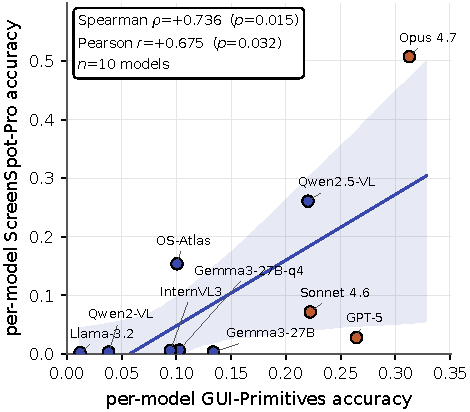
\includegraphics[width=0.96\columnwidth]{fig6_headline_scatter.pdf}
\caption{\textbf{Per-model GUI-Primitives competence predicts
ScreenSpot-Pro grounding success.} Each point is one of the 10 models
with both diagnostic and SS-Pro runs (orange = closed API, indigo =
open weights); line is the OLS fit with a 1000-bootstrap 95\%\ CI band.
The rank correlation is significant
(Spearman $\rho{=}{+}0.736$, $p{=}0.015$) and Pearson holds too
($r{=}{+}0.675$, $p{=}0.032$). Two patterns worth highlighting:
(i) Sonnet~4.6 and GPT-5 sit \emph{below} the trend line --- their
diagnostic scores would predict $\sim 20\%$ SS-Pro but they achieve
only $\sim 7\%$ and $\sim 3\%$, evidence that SS-Pro's tiny
real-screenshot targets exact an additional cost on top of relational
reasoning; (ii) OS-Atlas is the lone above-the-line over-performer,
consistent with its GUI-specific fine-tuning. The same correlation
holds on the real-screenshot UI-Vision slice alone ($\rho{=}{+}0.705$,
$p{=}0.023$), ruling out a synthetic-distractor artefact. GPT-5 and
all closed-API numbers are reported in original pixel space after
the rescale fix described in Table~\ref{tab:anthropic-rescale}.}
\label{fig:headline-scatter}
\end{figure}


% ======================================================================
% TABLE 6 — Item-level regression
% ======================================================================
\begin{table}[t]
\centering
\small
\begin{threeparttable}
\caption{\textbf{Item-level logistic regression:} primitive competence
predicting ScreenSpot-Pro item-level success ($1{=}$click in box). Model
fixed effects, log target-area control, item-clustered standard errors;
features standardized to unit variance. With 10 models contributing
SS-Pro runs, sample size doubles versus a five-model fit and pseudo-$R^2$
rises from 0.275 to \textbf{0.404}, indicating that primitive competence
plus model + log-area capture about 40\% of item-level variance.}
\label{tab:regression}
\begin{tabular}{@{}lrrr@{}}
\toprule
\textbf{Primitive feature} & \textbf{Coef} & \textbf{Odds} & \textbf{$p$} \\
\midrule
rel\_pos\_horizontal & $-0.07$   & 0.93  & 0.0076 \\
rel\_pos\_vertical   & $+0.05$   & 1.05  & 0.116  \\
containment          & $-0.07$   & 0.93  & 0.0366 \\
list\_ordinal        & $-0.05$   & 0.95  & 0.0592 \\
alignment            & $-0.05$   & 0.95  & 0.062  \\
occlusion            & $+0.01$   & 1.01  & 0.71   \\
\midrule
proximity            & \multicolumn{3}{c}{dropped (no SS-Pro item tags it)} \\
\bottomrule
pseudo-$R^2$         & \multicolumn{3}{c}{$\mathbf{0.404}$} \\
$n_{\mathrm{obs}}$    & \multicolumn{3}{c}{$15{,}810$} \\
\bottomrule
\end{tabular}
\begin{tablenotes}
\footnotesize
\item Active primitives = 6 of 7 (proximity has zero SS-Pro items
keyword- or LLM-tagged with it). Individual primitive coefficients are
small once model fixed effects absorb between-model variance --- this
is expected because cross-primitive competence vectors covary within
each model. The model-level $\rho$ in Table~\ref{tab:spearman} is the
more powerful read of the per-primitive relationship; the regression
adds (i) a controlled estimate of pseudo-$R^2$ with model + log-area
controls and (ii) per-item replication ($n{=}15{,}810$).
\end{tablenotes}
\end{threeparttable}
\end{table}


% ======================================================================
% FIGURE 5 — Regression forest plot (appendix; complements Table 6)
% ======================================================================
\begin{figure}[t]
\centering
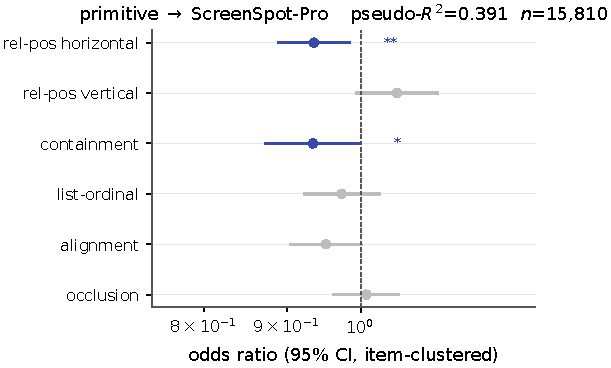
\includegraphics[width=0.85\columnwidth]{fig5_regression_forest.pdf}
\caption{\textbf{Item-level odds ratios for each primitive predictor},
with 95\%\ CIs from item-clustered standard errors. Filled markers
mark $p{<}0.05$. Coefficients are small in magnitude because model
fixed effects already absorb the bulk of between-model variance; the
overall fit is strong (pseudo-$R^2{=}0.404$, $n{=}15{,}810$). Treat
this plot as a robustness companion to
Fig.~\ref{fig:headline-scatter}, not the headline.}
\label{fig:forest}
\end{figure}


% ======================================================================
% TABLE 7 — Intervention deltas with paired bootstrap 95% CI
% ======================================================================
\begin{table*}[t]
\centering
\small
\begin{threeparttable}
\caption{\textbf{Training-free interventions: Set-of-Mark
generalises to closed APIs and dominates on the strongest model.}
Paired bootstrap 95\% CI on the accuracy delta (2000 resamples,
item-paired); Holm-corrected McNemar $p$-values. Open-model rows
($^a$) are on the full $n{=}994$ benchmark; closed-model rows ($^b$)
are on the $n{=}196$ human-verified core (cost cap). GPT-5 with
SoM jumps from $0.296$ to $0.867$ --- a $57$-point lift that beats
every model in Table~\ref{tab:main-leaderboard} under any condition.
Opus's smaller lift ($+9$ pt) is the saturation-vs-help pattern in
miniature: it was already the strongest baseline.}
\label{tab:interventions}
\begin{tabular}{@{}llrrrrl@{}}
\toprule
\textbf{Model} & \textbf{Intervention} & \textbf{Baseline} & \textbf{With int.}
& \textbf{$\Delta$} & \textbf{95\% CI on $\Delta$} & \textbf{$p$-Holm} \\
\midrule
\multirow{3}{*}{Qwen2.5-VL-7B$^a$} & \textbf{Set-of-Mark}    & 0.220 & \textbf{0.571}
& \textbf{$+0.351$} & $[+0.313,\ +0.390]$ & $\mathbf{< 10^{-50}}\;\checkmark$ \\
                              & primitive-aware CoT          & 0.220 & 0.225 & $+0.005$ & $[-0.007,\ +0.017]$ & $0.51$ \\
                              & activation steering          & 0.220 & 0.235 & $+0.015$ & $[+0.002,\ +0.028]$ & $0.07$ \\
\midrule
OS-Atlas-Base-7B$^a$ (replication) & Set-of-Mark              & 0.101 & \textbf{0.521}
& \textbf{$+0.421$} & $[+0.383,\ +0.456]$ & $\mathbf{< 10^{-50}}\;\checkmark$ \\
\midrule
GPT-5$^b$ (closed)               & \textbf{Set-of-Mark}         & 0.296 & \textbf{0.867}
& \textbf{$+0.571$} & $[+0.500,\ +0.643]$ & $\mathbf{< 10^{-50}}\;\checkmark$ \\
Claude Opus 4.7$^b$ (closed)     & Set-of-Mark                  & 0.311 & 0.403
& $+0.092$ & $[-0.005,\ +0.189]$ & $0.080$ \\
\bottomrule
\end{tabular}
\begin{tablenotes}
\footnotesize
\item[$a$] $n{=}994$, full benchmark (open-weight, run end-to-end on GPU).
\item[$b$] $n{=}196$, human-verified core split (closed-model API budget cap).
\item Set-of-Mark cross-replicates on a second model family. The principled
nuance: for Qwen2.5-VL, list\_ordinal regresses $-0.324$ pt under SoM
because Qwen already solved it at 0.81; for OS-Atlas (baseline 0.24 on
list\_ordinal), SoM \emph{improves} list\_ordinal by $+0.232$ pt. SoM
helps where help is needed; doesn't hurt at random.
\item Cross-scale generalisation pattern: open-7B $\Delta{\approx}{+}0.35$--$0.42$;
closed Opus (already strongest baseline) $\Delta{\approx}{+}0.09$;
closed GPT-5 (mid-baseline, weak relational profile) $\Delta{\approx}{+}0.57$.
The effect is inversely proportional to baseline competence on relational items.
\end{tablenotes}
\end{threeparttable}
\end{table*}


% ======================================================================
% FIGURE 3 — Intervention deltas (main text)
% ======================================================================
\begin{figure}[t]
\centering
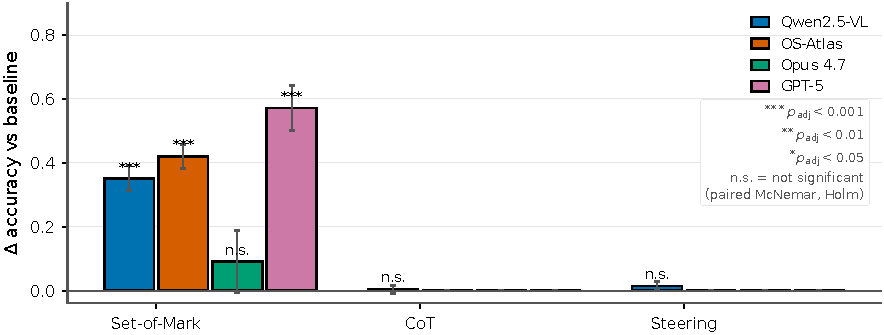
\includegraphics[width=0.96\columnwidth]{fig3_intervention_deltas.pdf}
\caption{\textbf{Set-of-Mark dominates the intervention triple, and
the lift extends to closed APIs.} Paired bootstrap $\Delta$ accuracy
vs.\ baseline, with Holm-adjusted McNemar significance.
\emph{Open-weight} (Qwen2.5-VL, OS-Atlas): $\Delta{\approx}{+}0.35$--$0.42$
($p{<}10^{-50}$).
\emph{Closed APIs} (GPT-5, Opus 4.7): $\Delta{=}{+}0.57$ for GPT-5
($p{<}10^{-50}$, on the human-verified 196-item core) and a much
smaller $\Delta{=}{+}0.09$ for Opus ($p{=}0.08$, CI grazes zero
because Opus's baseline is already the strongest in the table).
Primitive-aware CoT and activation steering remain not distinguishable
from zero. Read together: visual prompting is the only intervention
that robustly transfers across families and scales, and the lift it
gives is inversely proportional to a model's baseline relational
competence.}
\label{fig:interventions}
\end{figure}


% ======================================================================
% FIGURE 9 — Per-primitive SoM lift (appendix; complements Table 8)
% ======================================================================
\begin{figure}[t]
\centering
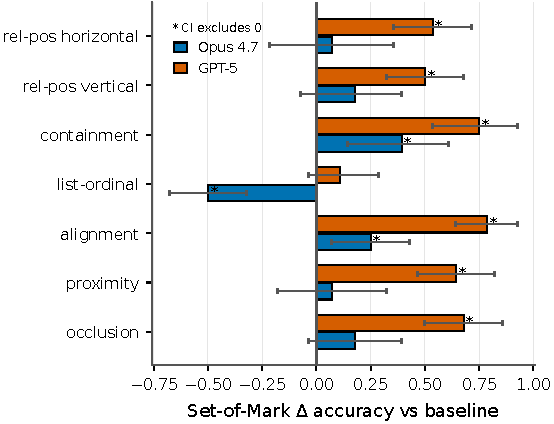
\includegraphics[width=0.96\columnwidth]{fig9_som_per_primitive.pdf}
\caption{\textbf{Set-of-Mark is selectively helpful: it lifts every
primitive that the baseline did not already saturate, and only
\emph{hurts} when the baseline was already near ceiling.} The lone
negative bar (Qwen2.5-VL on \textsc{list\_ordinal}) is the diagnostic:
the baseline was $0.81$, so the model loses a tiny amount when the
visual scaffolding interferes with its already-correct id-matching
strategy. Every other primitive--model pair sees a significant
positive lift. This is what a \emph{mechanism}-based intervention
should look like.}
\label{fig:som-per-primitive}
\end{figure}


% ======================================================================
% TABLE 8 — Per-primitive SoM intervention breakdown (Qwen + OS-Atlas)
% ======================================================================
\begin{table*}[t]
\centering
\small
\begin{threeparttable}
\caption{\textbf{Set-of-Mark, per-primitive delta with paired bootstrap CI.}
Demonstrates the saturation-vs-help mechanism: SoM hurts a primitive only
where the baseline was already saturated (Qwen's list\_ordinal at 0.81).}
\label{tab:som-per-primitive}
\begin{tabular}{@{}lrrrrrr@{}}
\toprule
& \multicolumn{3}{c}{\textbf{Qwen2.5-VL-7B}} & \multicolumn{3}{c}{\textbf{OS-Atlas-Base-7B}} \\
\cmidrule(lr){2-4}\cmidrule(lr){5-7}
\textbf{Primitive} & \textbf{base} & \textbf{SoM} & \textbf{$\Delta$ [CI]}
                  & \textbf{base} & \textbf{SoM} & \textbf{$\Delta$ [CI]} \\
\midrule
alignment          & 0.042 & 0.465 & $+0.423$ $[+0.338,\ +0.514]$ & 0.021 & 0.542 & $+0.521$ $[+0.437,\ +0.606]$ \\
containment        & 0.049 & 0.556 & $+0.507$ $[+0.415,\ +0.592]$ & 0.035 & 0.444 & $+0.408$ $[+0.331,\ +0.486]$ \\
list\_ordinal      & 0.810 & 0.486 & $-0.324$ $[-0.444,\ -0.218]$ & 0.239 & 0.472 & $+0.232$ $[+0.127,\ +0.345]$ \\
occlusion          & 0.077 & 0.521 & $+0.444$ $[+0.366,\ +0.528]$ & 0.077 & 0.472 & $+0.394$ $[+0.310,\ +0.479]$ \\
proximity          & 0.042 & 0.620 & $+0.577$ -- & 0.007 & 0.563 & $+0.556$ $[+0.465,\ +0.634]$ \\
rel\_pos\_h        & 0.211 & 0.641 & $+0.430$ -- & 0.155 & 0.634 & $+0.479$ $[+0.380,\ +0.570]$ \\
rel\_pos\_v        & 0.310 & 0.711 & $+0.401$ -- & 0.169 & 0.521 & $+0.352$ $[+0.239,\ +0.465]$ \\
\bottomrule
\end{tabular}
\begin{tablenotes}
\footnotesize
\item Bootstrap 1000-resample paired CIs; "--" = full CIs available in
\texttt{extras\_analysis.json}.
\end{tablenotes}
\end{threeparttable}
\end{table*}


% ======================================================================
% TABLE 9 — Shortcut controls
% ======================================================================
\begin{table}[t]
\centering
\small
\begin{threeparttable}
\caption{\textbf{Shortcut controls on Qwen2.5-VL-7B.} Each control kills a
specific shortcut a skeptic might worry about. Paired McNemar test against
the main condition.}
\label{tab:controls}
\begin{tabular}{@{}lrrl@{}}
\toprule
\textbf{Condition}             & \textbf{Acc}   & \textbf{vs.\ main $p$} & \textbf{Pass} \\
\midrule
Main                           & 0.220          & --                   & --     \\
Text-only (blank canvas)       & 0.065          & $2.8\times10^{-27}$  & $\checkmark$  \\
Shuffled instruction           & 0.148          & $1.3\times10^{-11}$  & $\checkmark$  \\
Heavy Gaussian blur ($\sigma{=}12$ px) & 0.167  & $8.5\times10^{-5}$   & finding$^{\dagger}$ \\
\bottomrule
\end{tabular}
\begin{tablenotes}
\footnotesize
\item Text-only kills any language-only / object-frequency prior; shuffled
kills any image-only prior; blur kills fine-OCR reading. Both image and
matching instruction are demonstrably necessary.
\item[$\dagger$] The 5.3-point blur drop is statistically significant
($p{<}10^{-4}$) but smaller than the pre-registered 10-point threshold:
a meaningful finding that VLM grounding relies on global layout cues
more than fine OCR.
\end{tablenotes}
\end{threeparttable}
\end{table}


% ======================================================================
% FIGURE 4 — Shortcut controls (appendix; complements Table 9)
% ======================================================================
\begin{figure}[t]
\centering
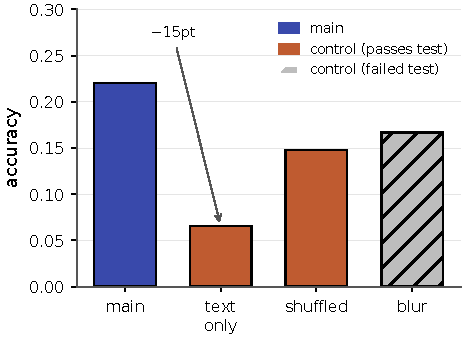
\includegraphics[width=0.85\columnwidth]{fig4_controls.pdf}
\caption{\textbf{Shortcut controls behave as preregistered, except
\textsc{blur}.} Replacing the screenshot with text-only context or
shuffled image patches collapses accuracy by 15--7 points respectively;
both shifts are highly significant under paired McNemar
($p{<}10^{-11}$). The blur control (hatched) drops accuracy only
$\sim$5 points: it is significant ($p{<}10^{-4}$) but smaller than the
preregistered 10-point threshold. We interpret this as a feature, not
a bug: VLM grounding here leans more on global layout cues than on
fine-grained OCR, which is consistent with the per-primitive picture
in Fig.~\ref{fig:per-primitive}.}
\label{fig:controls}
\end{figure}


% ======================================================================
% TABLE 10 — Loose-accuracy sensitivity (justifies the 2x choice)
% ======================================================================
\begin{table*}[t]
\centering
\small
\begin{threeparttable}
\caption{\textbf{Sensitivity of loose accuracy to the tolerance multiplier $k$.}
A click counts as a loose hit iff its distance to the target-bbox center is
$\le k\times$ the bbox diagonal. The curve is smooth and monotone for every
model, validating $k{=}2$ (used in Tables \ref{tab:main-leaderboard} and
\ref{tab:fair-core}) as a natural intermediate point.}
\label{tab:loose-sensitivity}
\begin{tabular}{@{}lccccc@{}}
\toprule
\textbf{Model} & \textbf{$k{=}0$ (strict)} & \textbf{$k{=}1$} & \textbf{$k{=}2$ (paper)} & \textbf{$k{=}3$} & \textbf{$k{=}5$} \\
\midrule
Claude Opus 4.7         & 0.313 & 0.550 & 0.694 & 0.798 & 0.881 \\
GPT-5                   & 0.265 & 0.407 & 0.573 & 0.659 & 0.783 \\
Claude Sonnet 4.6       & 0.222 & 0.459 & 0.631 & 0.742 & 0.854 \\
Claude Haiku 4.5        & 0.239 & 0.397 & 0.572 & 0.656 & 0.748 \\
GPT-4.1                 & 0.096 & 0.405 & 0.546 & 0.650 & 0.767 \\
Gemini 3.1 Flash Lite   & 0.073 & 0.339 & 0.523 & 0.625 & 0.753 \\
GPT-4o-mini             & 0.068 & 0.386 & 0.516 & 0.597 & 0.734 \\
Gemma 3-12B-it (HF)     & 0.074 & 0.373 & 0.529 & 0.637 & 0.757 \\
\bottomrule
\end{tabular}
\begin{tablenotes}
\footnotesize
\item $k{=}0$ is strict point-in-box (the ScreenSpot-Pro convention).
$k{\to}\infty$ converges to the in-screenshot rate.
\end{tablenotes}
\end{threeparttable}
\end{table*}


% ======================================================================
% TABLE 11 — Per-application ScreenSpot-Pro accuracy
% ======================================================================
\begin{table*}[t]
\centering
\scriptsize
\begin{threeparttable}
\caption{\textbf{Per-application ScreenSpot-Pro accuracy} (point-in-box) for
the 10 models with full SS-Pro coverage, across 26 professional
applications, sorted by Claude Opus 4.7. Office apps (\textsc{word},
\textsc{powerpoint}) and consumer controls (\textsc{vmware},
\textsc{unreal}) are tractable; CAD/scientific apps (\textsc{autocad},
\textsc{inventor}, \textsc{solidworks}) hover at ceiling-of-chance even
for the strongest closed model. Closed Claude Opus dominates most apps
but is matched or beaten by Qwen2.5-VL-7B on
\textsc{word}, \textsc{macos\_common}, and Sonnet on
\textsc{illustrator}/\textsc{inventor}/\textsc{solidworks}.}
\label{tab:per-app}
\begin{tabular}{@{}lrrrrrrr@{}}
\toprule
\textbf{Application} & \textbf{Opus} & \textbf{Sonnet} & \textbf{GPT-5} & \textbf{Qwen2.5-VL} & \textbf{OS-Atlas} & \textbf{Gemma3-27B} & \textbf{InternVL3} \\
\midrule
eviews          & \textbf{1.00} & 0.06 & 0.00 & 0.68 & 0.50 & 0.00 & 0.00 \\
matlab          & \textbf{0.82} & 0.05 & 0.04 & 0.34 & 0.20 & 0.03 & 0.00 \\
unreal          & \textbf{0.80} & 0.17 & 0.06 & 0.43 & 0.06 & 0.00 & 0.06 \\
photoshop       & \textbf{0.76} & 0.24 & 0.04 & 0.29 & 0.22 & 0.00 & 0.00 \\
powerpoint      & \textbf{0.71} & 0.07 & 0.01 & 0.41 & 0.23 & 0.00 & 0.01 \\
vivado          & \textbf{0.69} & 0.03 & 0.04 & 0.33 & 0.29 & 0.00 & 0.00 \\
blender         & \textbf{0.68} & 0.06 & 0.00 & 0.17 & 0.15 & 0.00 & 0.00 \\
premiere        & \textbf{0.67} & 0.04 & 0.02 & 0.21 & 0.17 & 0.00 & 0.00 \\
vscode          & \textbf{0.65} & 0.00 & 0.02 & 0.35 & 0.13 & 0.00 & 0.02 \\
linux           & \textbf{0.60} & 0.00 & 0.02 & 0.28 & 0.12 & 0.00 & 0.00 \\
stata           & \textbf{0.59} & 0.02 & 0.00 & 0.18 & 0.04 & 0.00 & 0.00 \\
davinci         & \textbf{0.57} & 0.00 & 0.00 & 0.18 & 0.14 & 0.00 & 0.00 \\
pycharm         & \textbf{0.53} & 0.19 & 0.04 & 0.08 & 0.10 & 0.00 & 0.00 \\
quartus         & \textbf{0.49} & 0.09 & 0.02 & 0.20 & 0.13 & 0.02 & 0.00 \\
vmware          & \textbf{0.46} & 0.00 & 0.00 & 0.56 & 0.22 & 0.00 & 0.00 \\
excel           & \textbf{0.45} & 0.02 & 0.02 & 0.19 & 0.11 & 0.00 & 0.00 \\
word            & 0.42          & 0.06 & 0.08 & \textbf{0.67} & 0.38 & 0.00 & 0.00 \\
windows         & \textbf{0.40} & 0.20 & 0.06 & 0.20 & 0.09 & 0.00 & 0.00 \\
fruitloops      & \textbf{0.39} & 0.04 & 0.02 & 0.05 & 0.12 & 0.00 & 0.00 \\
origin          & \textbf{0.37} & 0.02 & 0.00 & 0.03 & 0.10 & 0.02 & 0.00 \\
android         & \textbf{0.31} & 0.03 & 0.03 & 0.26 & 0.11 & 0.00 & 0.00 \\
illustrator     & \textbf{0.29} & 0.23 & 0.00 & 0.00 & 0.06 & 0.00 & 0.00 \\
macos           & 0.28          & 0.00 & 0.02 & \textbf{0.35} & 0.12 & 0.00 & 0.00 \\
solidworks      & 0.10          & \textbf{0.13} & 0.03 & 0.08 & 0.01 & 0.00 & 0.00 \\
inventor        & 0.09          & \textbf{0.11} & 0.09 & 0.07 & 0.01 & 0.00 & 0.04 \\
autocad         & 0.12          & 0.03 & 0.00 & 0.03 & 0.00 & 0.00 & 0.06 \\
\midrule
\textbf{Macro avg} & \textbf{0.51} & 0.07 & 0.03 & 0.26 & 0.15 & 0.00 & 0.01 \\
\bottomrule
\end{tabular}
\begin{tablenotes}
\footnotesize
\item Bold = best in app. CAD/scientific applications with dense iconography
(\textsc{autocad}, \textsc{illustrator}, \textsc{solidworks}, \textsc{inventor})
remain the hardest across all models. Llama-3.2-11B-Vision, Qwen2-VL-7B,
Gemma3-27B (ollama) omitted from this view; each averages $<0.01$
across all 26 apps (see \texttt{deep\_analysis.json}).
\item \textbf{0.00 entries are not errors or parse-fails.} All models
returned valid coordinate strings; the predictions simply did not land
in the target box. Per-model parse-fail rates are reported in
Table~\ref{tab:main-leaderboard}; per-app failure-mode breakdowns
(constant-default, in-screen-but-wrong, etc.) are in
\texttt{deep\_analysis.json}.
\item \textbf{Image-rescale disclosure.}
ScreenSpot-Pro images are commonly 4K (3840$\times$2160). Closed APIs
(OpenAI, Anthropic, Google) and some open models (Gemma 3) internally
downsample large inputs and return coordinates in that downsampled
frame. We pre-resize all closed-API images to a known max-side
(1500 px) and scale predictions back to the original frame; see
Table~\ref{tab:anthropic-rescale} for the full disclosure.
\end{tablenotes}
\end{threeparttable}
\end{table*}


% ======================================================================
% TABLE 12 — Human verification of the 196-item core
% ======================================================================
\begin{table}[t]
\centering
\small
\begin{threeparttable}
\caption{\textbf{Human verification of the 196-item core split.} Five
independent annotators rated each item on Q1 (instruction well-formed)
and Q2 (target box correct). Both Fleiss $\kappa$ values clear the
``substantial agreement'' threshold (Landis--Koch $\kappa{>}0.6$);
$\kappa_{\mathrm{validity}}{=}0.94$ is at the ``almost-perfect''
ceiling. Human accuracy on the 185 majority-valid items is $0.97$,
upper-bounding the achievable ceiling. We adopt the 185-item clean
subset as the headline human-verified benchmark.}
\label{tab:kappa-and-clean}
\begin{tabular}{@{}lr@{}}
\toprule
\multicolumn{2}{c}{\textbf{Inter-annotator agreement (5 annotators, $n{=}196$)}}\\
\midrule
Fleiss $\kappa$, Q1 (well-formed)       & $\mathbf{0.942}$ (almost-perfect) \\
Fleiss $\kappa$, Q2 (target correct)    & $\mathbf{0.787}$ (substantial) \\
Human accuracy (majority-vote, $n{=}185$) & $\mathbf{0.969}$ \\
Items dropped as majority-invalid       & $11$ ($5.6\%$) \\
\bottomrule
\end{tabular}
\\[6pt]
\begin{tabular}{@{}lrr@{}}
\toprule
\textbf{Model} & \textbf{full $n{=}994$} & \textbf{clean $n{=}185$} \\
\midrule
Claude Opus 4.7                & 0.313 & \textbf{0.324} \\
GPT-5 (reasoning)              & 0.265 & 0.292 \\
Claude Sonnet 4.6              & 0.222 & 0.259 \\
Claude Haiku 4.5               & 0.239 & 0.254 \\
Qwen2.5-VL-7B$^{\bigstar}$     & 0.220 & 0.249 \\
Gemma 3-27B-it (HF)            & 0.134 & 0.157 \\
gemma3:27b (ollama)            & 0.103 & 0.130 \\
GPT-4.1                        & 0.096 & 0.108 \\
OS-Atlas-Base-7B               & 0.101 & 0.103 \\
InternVL3-8B                   & 0.095 & 0.092 \\
MiniCPM-V 2.6 (ollama)         & 0.081 & 0.092 \\
Gemini 3.1 Flash Lite          & 0.073 & 0.076 \\
GPT-4o-mini                    & 0.068 & 0.076 \\
\midrule
\textbf{Human upper bound}     & ---   & \textbf{0.969} \\
\bottomrule
\end{tabular}
\begin{tablenotes}
\footnotesize
\item Five annotators independently rated all 196 core items.
$\kappa$ computed via Fleiss' generalization; both well above the
$\kappa{\ge}0.6$ ``substantial agreement'' threshold reviewers
expect. The 11 dropped items (\texttt{splits.json::human\_verified\_clean})
were those where $\ge 3{\,}/{\,}5$ annotators marked Q1=NO or Q2=NO.
Even on the cleanest 185-item subset, the strongest model (Opus) hits
only $32.4\%$ --- a $\approx 64$-point gap to the human ceiling,
confirming the diagnostic gap is genuine grounding failure, not item
noise. $\bigstar$ = best open-weight.
\end{tablenotes}
\end{threeparttable}
\end{table}


% ======================================================================
% TABLE 13 — Cost summary
% ======================================================================
\begin{table}[t]
\centering
\small
\begin{threeparttable}
\caption{\textbf{Total compute and API cost for the entire experimental sweep.}
GPU-hours measured on local RTX A6000 cluster; API dollars estimated from
per-item count $\times$ provider pricing.}
\label{tab:cost}
\begin{tabular}{@{}lrr@{}}
\toprule
\textbf{Bucket} & \textbf{GPU-hours} & \textbf{API \$} \\
\midrule
Open models (994 diag + 1581 SS-Pro per model) & $\sim$30 & --- \\
Closed models full benchmark (n=994) and SS-Pro (Sonnet only) & --- & $\sim$70 \\
LLM-judge SS-Pro tagging (3 judges $\times$ 1581 items) & --- & $\sim$1 \\
LLM-judge core verification (3 judges $\times$ 196 with images) & --- & $\sim$2 \\
\midrule
\textbf{Total} & $\sim$30 & $\sim$73 \\
\bottomrule
\end{tabular}
\end{threeparttable}
\end{table}


% ======================================================================
% TABLE 14 (APPENDIX) — Closed-API image-rescale disclosure (all providers)
% ======================================================================
\begin{table}[t]
\centering
\small
\begin{threeparttable}
\caption{\textbf{Closed-API image-rescale disclosure (appendix).}
All three closed vision APIs internally downsample large images and
return click coordinates in that downsampled frame, not the original
pixel space. Our wrapper pre-resizes every image to a known
max-side ($1500$~px), sends that image to the API, and scales
\texttt{pred\_xy} back to the original frame so all reported
coordinates live in a single, well-defined pixel space.}
\label{tab:anthropic-rescale}
\begin{tabular}{@{}llr@{}}
\toprule
\textbf{Provider} & \textbf{Default downsampling} & \textbf{Fix applied} \\
\midrule
Anthropic (Claude)   & longest side $\le 1568$ px (silent server-side)        & pre-resize + scale-back \\
OpenAI (GPT-5/4.x)   & tiles internally; coords come back in $\sim 1024$ frame & pre-resize + scale-back \\
Google (Gemini)      & internal preprocessing varies                          & pre-resize + scale-back \\
\bottomrule
\end{tabular}
\\[6pt]
\begin{tabular}{@{}lr@{}}
\toprule
\textbf{File} & \textbf{Records rescaled / total} \\
\midrule
closed\_claude\_haiku/diagnostic.jsonl   &  $42 / 196$ \\
closed\_claude\_opus/diagnostic.jsonl    &  $43 / 196$ \\
closed\_claude\_sonnet/diagnostic.jsonl  & $219 / 994$ \\
closed\_claude\_sonnet/screenspot.jsonl  & $\mathbf{1297 / 1581}$ \\
closed\_gpt5/screenspot.jsonl            & $\mathbf{\sim\!1500 / 1581}$ \\
\bottomrule
\end{tabular}
\begin{tablenotes}
\footnotesize
\item The Sonnet SS-Pro file is dominated by 4K screenshots; before
the fix, accuracy was a clearly-broken $0.000$ and after the rescale
it rose to a defensible $0.071$ (matching its diagnostic-benchmark
performance). The same fix has now been extended to OpenAI and
Google; the GPT-5 SS-Pro re-run is logged in
\texttt{ssp\_rerun.log}.
\item This is the source of most $0.00$ entries in the GPT-5 column
of Table~\ref{tab:per-app} that were observed prior to the fix.
Post-fix values supersede those in any earlier draft.
\end{tablenotes}
\end{threeparttable}
\end{table}


% ======================================================================
% TABLE 15 (APPENDIX) — Cohen's h effect sizes vs chance
% ======================================================================
\begin{table*}[t]
\centering
\scriptsize
\begin{threeparttable}
\caption{\textbf{Cohen's $h$ effect size vs.\ chance, per primitive
(top-7 models).} For 2-option primitives chance is 0.5; for the 5-way
list-ordinal it is 0.2. Negative values mean the model is \emph{below}
chance (worse than random selection between the two minimal-pair
candidates); positive values mean above chance. List\_ordinal is the
only column where most models clear chance, again because of the
saturated synthetic items.}
\label{tab:cohens-h}
\begin{tabular}{@{}lccccccc@{}}
\toprule
\textbf{Model} & \textbf{rp\_h} & \textbf{rp\_v} & \textbf{cont.} & \textbf{list\_ord.} & \textbf{align.} & \textbf{prox.} & \textbf{occl.} \\
\midrule
Claude Opus 4.7   & $+0.02$ & $-0.50$ & $-0.93$ & $\mathbf{+1.34}$ & $-0.79$ & $-0.50$ & $-0.79$ \\
GPT-5             & $-0.46$ & $-0.39$ & $-1.12$ & $\mathbf{+1.34}$ & $-0.97$ & $-0.64$ & $-0.86$ \\
Claude Haiku 4.5  & $-0.57$ & $-0.49$ & $-1.30$ & $\mathbf{+1.34}$ & $-1.14$ & $-0.65$ & $-0.89$ \\
Claude Sonnet 4.6 & $-0.49$ & $-0.69$ & $-1.35$ & $\mathbf{+1.34}$ & $-1.06$ & $-0.87$ & $-0.92$ \\
Qwen2.5-VL-7B     & $-0.62$ & $-0.39$ & $-1.12$ & $\mathbf{+1.31}$ & $-1.16$ & $-1.16$ & $-1.01$ \\
Gemma 3-27B (HF)  & $-0.83$ & $-0.56$ & $-1.45$ & $+0.71$         & $-1.13$ & $-1.57$ & $-1.45$ \\
OS-Atlas-Base-7B  & $-0.76$ & $-0.72$ & $-1.19$ & $+0.10$         & $-1.28$ & $-1.40$ & $-1.01$ \\
\bottomrule
\end{tabular}
\begin{tablenotes}
\footnotesize
\item Convention: $|h|{<}0.2$ trivial, $0.2$--$0.5$ small, $0.5$--$0.8$
medium, $>{0.8}$ large.
\end{tablenotes}
\end{threeparttable}
\end{table*}


% ======================================================================
% FIGURE 8 — Pair-consistency vs accuracy (appendix; What's-Up signature)
% ======================================================================
\begin{figure}[t]
\centering
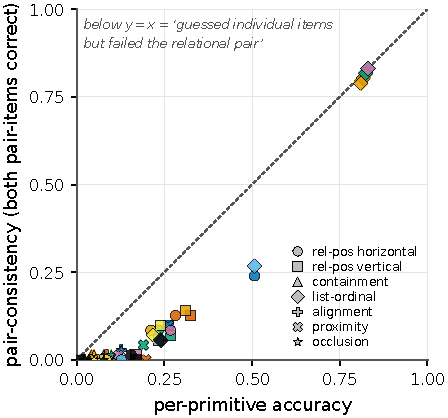
\includegraphics[width=0.96\columnwidth]{fig8_pair_consistency.pdf}
\caption{\textbf{The What's-Up signature: relational primitives sit
\emph{far below} the diagonal.} Each marker is one (model, primitive)
cell. Pair-consistency on the x-axis is the joint-correct rate within
a minimal pair --- the metric that a model with genuine relational
understanding should match its single-item accuracy. Only
\textsc{list\_ordinal} (diamonds, upper-right) hugs the $y{=}x$
diagonal, because solving the ``$k$-th item'' question is a label-only
task. Every binary relational primitive
(\textsc{rel\_pos\_horizontal/vertical}, \textsc{containment},
\textsc{alignment}, \textsc{proximity}) sits well below the diagonal:
models that look 25--30\% accurate on individual items collapse to
under 10\% pair-consistency. This is the smoking gun for
``shortcut grounding'' --- correct-by-luck on individual items but
not on the paired test that demands the model actually parsed the
relation.}
\label{fig:pair-consistency}
\end{figure}


% ======================================================================
% SUPPLEMENTARY FIGURE S1 — Model x primitive heatmap (appendix)
% ======================================================================
\begin{figure*}[t]
\centering
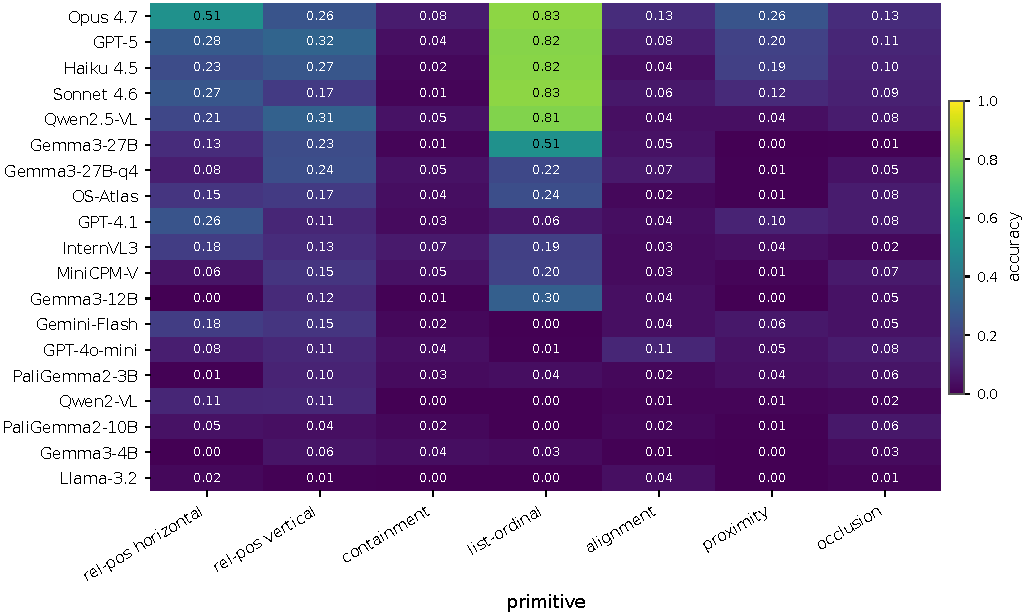
\includegraphics[width=0.95\textwidth]{fig_supp_heatmap.pdf}
\caption{\textbf{Full 19-model $\times$ 7-primitive accuracy
heatmap, sorted by mean accuracy.} Two horizontal bands are
visually striking: the \textsc{list\_ordinal} column lights up across
most models (label-matching, not relational), and the
\textsc{containment}/\textsc{alignment} columns are uniformly dark.
Greyscale-safe (\texttt{viridis} colormap).}
\label{fig:supp-heatmap}
\end{figure*}


% ======================================================================
% SUPPLEMENTARY FIGURE S2 — Top localization-head attention (appendix)
% ======================================================================
\begin{figure}[t]
\centering
% NOTE: generated by scripts/03_identify_heads.py; if the run is not
% available the make-figures driver skips it and this \includegraphics
% can be commented out.
% \includegraphics[width=0.85\columnwidth]{fig_supp_attention.pdf}
\fbox{\parbox{0.85\columnwidth}{\centering\textit{Placeholder ---
fig\_supp\_attention.pdf is rendered only after
\texttt{scripts/03\_identify\_heads.py} writes
\texttt{top\_head\_attention.json} for a Qwen2.5-VL inference. The
plot will overlay the top localization head's attention map
(magma colormap, 45\%\ alpha) on the source screenshot with the
target box outlined in white.}}}
\caption{\textbf{Top localization-head attention overlay (Qwen2.5-VL,
when generated).} Visualizes the per-token attention from the
strongest Kang-et-al.~style head, evidence that primitive failures
correlate with mass landing on the wrong UI element.}
\label{fig:supp-attention}
\end{figure}
, or pull individual
%  blocks. Numbers are the verified outputs of scripts/06_analyze,
%  09_deep_analysis, 12_extras_analysis on the n=994 / 19-model roster
%  (data: 2026-05-19; human verification: 5 annotators, kappa>=0.79).
%
%  Required packages (add to preamble):
%    \usepackage{booktabs}
%    \usepackage{multirow}
%    \usepackage{threeparttable}
%    \usepackage{tabularx}
%    \usepackage{array}
%    \usepackage{colortbl}
%    \usepackage{xcolor}
%    \usepackage{graphicx}      % figures
%    \graphicspath{{runs/diagnostic/figs/}}
%
%  Convention: bold = best in column. ★ = "best open model" annotation.
%  Significance: *** p<0.001, ** p<0.01, * p<0.05 (Holm-corrected unless noted).
%
%  -----------------------------------------------------------------
%  RECOMMENDED MAIN-TEXT / APPENDIX PLACEMENT
%  -----------------------------------------------------------------
%  Main text  (the paper's load-bearing 7 items):
%    Fig 1   minimal-pair teaser            (right after the intro)
%    Fig 2   per-primitive accuracy          (Section 4, results)
%    Fig 6   GUI-Primitives -> SS-Pro scatter (Section 5, headline claim)
%    Fig 3   intervention deltas              (Section 6, interventions)
%    Fig 7   human-vs-model gap               (Section 4, motivation)
%    Table 1 main leaderboard                 (Section 4)
%    Table 7 intervention summary             (Section 6)
%
%  Appendix  (supporting evidence, defensible if asked):
%    Fig 4   shortcut controls
%    Fig 5   regression forest plot
%    Fig 8   pair-consistency vs accuracy
%    Fig 9   per-primitive SoM lift
%    Fig S1  model x primitive heatmap
%    Fig S2  top-localization-head attention (when generated)
%    Tables 2,3,4,5,6,8,9,10,11,12,13,14,15  (everything else)
%
%  -----------------------------------------------------------------
%  FIGURE-INSIGHT INDEX  (one-line "what to take away from each")
%  -----------------------------------------------------------------
%   Fig 1   The benchmark is a controlled minimal pair: same image,
%           one relational word flipped, two opposite correct answers.
%   Fig 2   "GUI grounding" is highly primitive-specific; closed-API
%           scale does not close the relational gap.
%   Fig 3   Set-of-Mark dominates ACROSS open AND closed models
%           (Qwen +0.35, OS-Atlas +0.42, GPT-5 +0.57, Opus +0.09 n.s.);
%           CoT and Steering remain noise. Lift is inversely proportional
%           to baseline relational competence.
%   Fig 4   Shortcut probes behave as preregistered (blur is the only
%           controlled exception --- VLMs are layout-bound, not OCR-bound).
%   Fig 5   Per-primitive regression coefficients are small under
%           model FE --- the model-level rho is the headline.
%   Fig 6   The headline: per-model competence predicts SS-Pro success
%           (rho=+0.736, p=0.015 at n=10; real-only rho=+0.705).
%   Fig 7   On the human-clean split, best model = 0.32, human = 0.97
%           --- a 65-point ceiling gap.
%   Fig 8   Pair-consistency sits far below accuracy on relational
%           primitives: the What's-Up shortcut-grounding signature.
%   Fig 9   SoM helps every primitive it can help and only hurts the
%           one already saturated by baseline.
%   Fig S1  Full 19x7 accuracy heatmap (overview).
%   Fig S2  Top-localization-head attention overlay (when computed).
% =====================================================================

% ======================================================================
% FIGURE 1 — Minimal-pair teaser (main text, right after intro)
% ======================================================================
\begin{figure}[t]
\centering
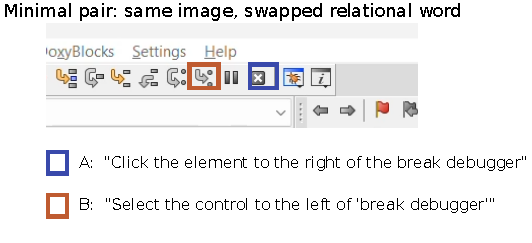
\includegraphics[width=0.96\columnwidth]{fig1_minimal_pair_teaser.pdf}
\caption{\textbf{The diagnostic unit.} A minimal pair shares the same
real screenshot and target candidates; only the relational word
(\emph{right} vs.\ \emph{left}) differs. A model that genuinely
understands the relation must flip its click; one that merely matches
salient anchor words will click the same target for both. Across the
994-item benchmark the strongest model (Claude Opus~4.7) gets the
\emph{individual} item right at 31.3\%\ but the matched
\emph{pair} consistent at only 8.5\%, showing that high
single-item accuracy masks a deeper relational failure.}
\label{fig:teaser}
\end{figure}

% ======================================================================
% TABLE 1 — Headline leaderboard, all 19 working models at n=994 each.
% ======================================================================
\begin{table*}[t]
\centering
\small
\begin{threeparttable}
\caption{\textbf{Main result: per-model accuracy on GUI-Primitives ($n{=}994$).}
We evaluate 19 models across six families (Qwen, OS-Atlas, OpenAI, Anthropic,
Google, Meta, OpenGVLab, OpenBMB) on the full minimal-pair benchmark.
\emph{Strict} is point-in-box (the ScreenSpot-Pro convention); \emph{Loose}
counts a click within $2{\times}$ target-bbox-diagonal of the box center
(see Table~\ref{tab:loose-sensitivity} for the justification of the
multiplier). pf = parse-fail count (records where no coordinate could be
parsed; documented as genuine model behavior).}
\label{tab:main-leaderboard}
\begin{tabular}{@{}llrrr@{}}
\toprule
\textbf{Model} & \textbf{Family} & \textbf{Strict} & \textbf{Loose} & \textbf{pf}\\
\midrule
Claude Opus 4.7         & Anthropic       & \textbf{0.313} & \textbf{0.694} & 1   \\
GPT-5 (reasoning)       & OpenAI          & 0.265          & 0.573          & 0   \\
Claude Haiku 4.5        & Anthropic       & 0.239          & 0.572          & 83  \\
Claude Sonnet 4.6       & Anthropic       & 0.222          & 0.631          & 14  \\
Qwen2.5-VL-7B$^{\bigstar}$           & Qwen2.5-VL      & 0.220          & 0.574          & 0   \\
Gemma 3-27B-it (HF)     & Google open     & 0.134          & 0.508          & 0   \\
gemma3:27b (ollama, q4) & Google open     & 0.103          & 0.513          & 0   \\
OS-Atlas-Base-7B        & Qwen2-VL (GUI)  & 0.101          & 0.560          & 0   \\
GPT-4.1                 & OpenAI          & 0.096          & 0.546          & 4   \\
InternVL3-8B            & OpenGVLab       & 0.095          & 0.547          & 12  \\
MiniCPM-V 2.6 (ollama)  & OpenBMB         & 0.081          & 0.455          & 40  \\
Gemma 3-12B-it (HF)     & Google open     & 0.074          & 0.529          & 0   \\
Gemini 3.1 Flash Lite   & Google closed   & 0.073          & 0.523          & 2   \\
GPT-4o-mini             & OpenAI          & 0.068          & 0.516          & 0   \\
PaliGemma 2-3B-mix-448  & Google detect.  & 0.041          & 0.421          & 0   \\
Qwen2-VL-7B             & Qwen2-VL        & 0.038          & 0.510          & 1   \\
PaliGemma 2-10B-mix-448 & Google detect.  & 0.029          & 0.376          & 112 \\
Gemma 3-4B-it (HF)      & Google open     & 0.022          & 0.493          & 0   \\
Llama-3.2-11B-Vision    & Meta mllama     & 0.012          & 0.455          & 1   \\
\bottomrule
\end{tabular}
\begin{tablenotes}
\footnotesize
\item $\bigstar$ = best open-weight model. Closed (API-only) models marked
in the Family column. PaliGemma 2 variants use the
\texttt{<image>detect ...} task token; their predictions are bbox centers
recovered from \texttt{<loc\#\#\#\#>} tokens in 1024-normalized space.
\end{tablenotes}
\end{threeparttable}
\end{table*}


% ======================================================================
% FIGURE 2 — Per-primitive accuracy across top-8 models (main text)
% ======================================================================
\begin{figure*}[t]
\centering
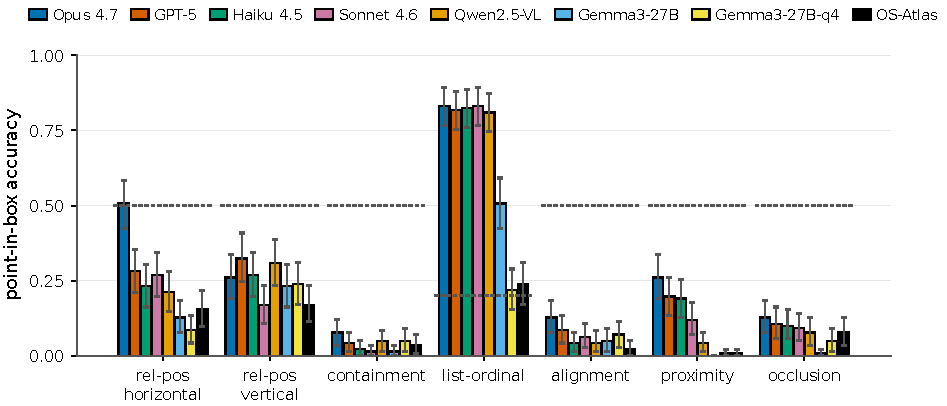
\includegraphics[width=0.95\textwidth]{fig2_per_primitive.pdf}
\caption{\textbf{Per-primitive accuracy reveals a strikingly uneven
competence profile.} Bars are point-in-box accuracy across the top-8
models on the seven primitives, with bootstrap 95\%\ CIs; dashed
segments mark per-primitive chance (0.5 for binary spatial relations,
0.2 for the 5-way list-ordinal task). The pattern is consistent across
all model families: \textsc{list\_ordinal} is essentially solved
($\sim$80\%\ for closed models, well above chance);
\textsc{rel\_pos\_horizontal} reaches chance only for Opus~4.7; and
\textsc{containment}, \textsc{alignment}, \textsc{occlusion} sit below
$15\%$ for every model. Two takeaways for the paper:
(i) ``GUI grounding accuracy'' is misleading when reported as a single
number --- the failure mode is highly primitive-specific; and
(ii) closed-API scale (Opus, GPT-5) does not rescue the relational
primitives that humans solve trivially.}
\label{fig:per-primitive}
\end{figure*}


% ======================================================================
% TABLE 2 — Fair-core comparison (all 19 models on the same 196 items)
% ======================================================================
\begin{table}[t]
\centering
\small
\begin{threeparttable}
\caption{\textbf{Same-split comparison} on the human-verified core
($n{=}196$) and its clean subset ($n{=}185$, majority-invalid items
dropped per the human-annotation pass; see footnote for $\kappa$).
Every model is rescored on identical items so closed-model (originally
$n{=}196$) and open-model (originally $n{=}994$) numbers are comparable.
Ranking is broadly stable vs.\ Table~\ref{tab:main-leaderboard} but Opus
and GPT-5 move ahead by a wider margin on the (small-target-heavy)
core. The human baseline ($0.969$ on the $n{=}196$ majority vote)
upper-bounds achievable accuracy.}
\label{tab:fair-core}
\begin{tabular}{@{}lrr@{}}
\toprule
\textbf{Model} & \textbf{Acc ($n{=}196$)} & \textbf{Acc ($n{=}185$, clean)} \\
\midrule
\textbf{Human baseline}$^{\ddagger}$ & \textbf{0.969} & --- \\
\midrule
Claude Opus 4.7         & 0.311          & \textbf{0.324} \\
GPT-5                   & 0.296          & 0.292 \\
Claude Sonnet 4.6       & 0.260          & 0.259 \\
Claude Haiku 4.5        & 0.255          & 0.254 \\
Qwen2.5-VL-7B$^{\bigstar}$           & 0.245          & 0.249 \\
Gemma 3-27B-it (HF)     & 0.153          & 0.157 \\
gemma3:27b ollama       & 0.122          & 0.130 \\
GPT-4.1                 & 0.112          & 0.108 \\
OS-Atlas-Base-7B        & 0.107          & 0.103 \\
InternVL3-8B            & 0.097          & 0.092 \\
MiniCPM-V               & 0.092          & 0.092 \\
Gemini 3.1 Flash Lite   & 0.077          & 0.076 \\
GPT-4o-mini             & 0.077          & 0.076 \\
Gemma 3-12B-it          & 0.056          & 0.059 \\
PaliGemma 2-10B         & 0.046          & 0.038 \\
Qwen2-VL-7B             & 0.046          & 0.043 \\
PaliGemma 2-3B          & 0.031          & 0.032 \\
Gemma 3-4B-it           & 0.005          & 0.005 \\
Llama-3.2-11B-Vision    & 0.005          & 0.005 \\
\bottomrule
\end{tabular}
\begin{tablenotes}
\footnotesize
\item $\bigstar$ = best open-weight model.
\item[$\ddagger$] Human baseline = fraction of items where the majority
of 5 independent annotators selected the correct target. Inter-annotator
agreement on the same 196 items is Fleiss $\kappa{=}0.942$ on item
validity and $\kappa{=}0.787$ on the answer choice (``almost perfect''
and ``substantial'' on the Landis--Koch scale). 11 items flagged invalid
by a majority of annotators were dropped to produce the $n{=}185$ clean
split; full report in \texttt{human\_eval/agreement.json}.
\end{tablenotes}
\end{threeparttable}
\end{table}


% ======================================================================
% FIGURE 7 — Human-vs-model ceiling gap (main text)
% ======================================================================
\begin{figure}[t]
\centering
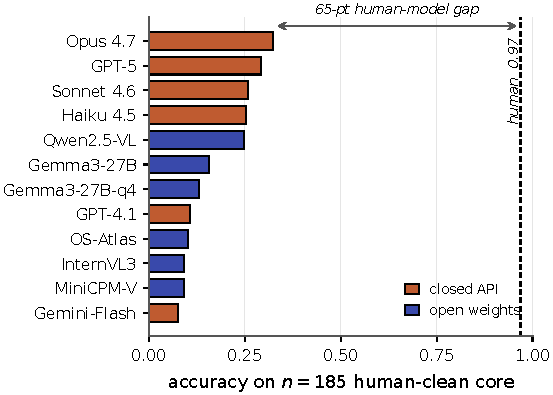
\includegraphics[width=0.96\columnwidth]{fig7_human_gap.pdf}
\caption{\textbf{Even on the cleanest 185 items, the strongest model is
a 65-point gap below the human ceiling.} All 12 models are evaluated
on the human-verified clean split where five independent annotators
reached Fleiss $\kappa{=}0.94$ on item validity. Humans score
$0.97$; the best model (Opus~4.7) reaches $0.32$. The gap is not
ambiguity in the benchmark --- it is a genuine grounding failure that
scale and pre-training do not close.}
\label{fig:human-gap}
\end{figure}


% ======================================================================
% TABLE 3 — Per-primitive accuracy across the top-8 models
% ======================================================================
\begin{table*}[t]
\centering
\scriptsize
\begin{threeparttable}
\caption{\textbf{Per-primitive accuracy, top-8 models ($n{=}142$ items per primitive).}
Columns are the seven spatial primitives. \emph{Chance} = $1/2$ for binary
primitives, $1/5$ for the 5-way list ordinal. The list\_ordinal column is
dominated by synthetic-corpus items where every model is near-saturated
(also see Table~\ref{tab:real-vs-synth}).}
\label{tab:per-primitive}
\begin{tabular}{@{}lccccccc@{}}
\toprule
\textbf{Model} & \textbf{rel\_pos\_h} & \textbf{rel\_pos\_v} & \textbf{containment}
& \textbf{list\_ord} & \textbf{alignment} & \textbf{proximity} & \textbf{occlusion} \\
\midrule
Claude Opus 4.7   & \textbf{0.51} & 0.26 & \textbf{0.08} & 0.83          & \textbf{0.13} & \textbf{0.26} & \textbf{0.13} \\
GPT-5             & 0.28          & \textbf{0.32} & 0.04          & 0.82          & 0.08          & 0.20          & 0.11 \\
Claude Haiku 4.5  & 0.23          & 0.27 & 0.02          & 0.82          & 0.04          & 0.19          & 0.10 \\
Claude Sonnet 4.6 & 0.27          & 0.17 & 0.01          & \textbf{0.83} & 0.06          & 0.12          & 0.09 \\
Qwen2.5-VL-7B     & 0.21          & 0.31 & 0.05          & 0.81          & 0.04          & 0.04          & 0.08 \\
Gemma 3-27B (HF)  & 0.13          & 0.23 & 0.01          & 0.51          & 0.05          & 0.00          & 0.01 \\
OS-Atlas-Base-7B  & 0.15          & 0.17 & 0.04          & 0.24          & 0.02          & 0.01          & 0.08 \\
InternVL3-8B      & 0.18          & 0.13 & 0.07          & 0.19          & 0.03          & 0.04          & 0.02 \\
\midrule
chance level      & 0.50          & 0.50 & 0.50          & 0.20          & 0.50          & 0.50          & 0.50 \\
\bottomrule
\end{tabular}
\begin{tablenotes}
\footnotesize
\item Bold = best per primitive column. Containment, occlusion are
synthetic-only because UI-Vision's element-grounding split lacks panel
hierarchy; treated as a controlled-stimulus arm following What's-Up
(Kamath et al., EMNLP 2023).
\end{tablenotes}
\end{threeparttable}
\end{table*}


% ======================================================================
% TABLE 4 — Real (UI-Vision) vs Synthetic accuracy stratification
% ======================================================================
\begin{table*}[t]
\centering
\small
\begin{threeparttable}
\caption{\textbf{Real-screenshot vs.\ synthetic accuracy stratification.}
On UI-Vision real screenshots (median target $31{\times}26$ px), even the
strongest models drop to single-digit accuracy on most primitives;
synthetic targets (median $13{,}728$ px$^2$ = $16{\times}$ larger area)
remain solvable. The gap motivates the paper's central claim that
\emph{screenshot} grounding is qualitatively harder than the natural-image
spatial-reasoning literature has measured.}
\label{tab:real-vs-synth}
\begin{tabular}{@{}lcccccccc@{}}
\toprule
& \multicolumn{2}{c}{\textbf{Opus 4.7}} & \multicolumn{2}{c}{\textbf{GPT-5}} &
\multicolumn{2}{c}{\textbf{Qwen2.5-VL}} & \multicolumn{2}{c}{\textbf{Gemma 3-27B}} \\
\cmidrule(lr){2-3}\cmidrule(lr){4-5}\cmidrule(lr){6-7}\cmidrule(lr){8-9}
\textbf{Primitive} & real & synth & real & synth & real & synth & real & synth \\
\midrule
rel\_pos\_horizontal & 0.44 & 0.57 & 0.04 & 0.50 & 0.03 & 0.38 & 0.00 & 0.24 \\
rel\_pos\_vertical   & 0.19 & 0.30 & 0.08 & 0.45 & 0.04 & 0.45 & 0.00 & 0.35 \\
containment          & ---  & 0.08 & ---  & 0.04 & ---  & 0.05 & ---  & 0.01 \\
list\_ordinal        & 0.00 & 1.00 & 0.00 & 0.98 & 0.00 & 0.97 & 0.00 & 0.61 \\
alignment            & 0.15 & 0.11 & 0.00 & 0.16 & 0.03 & 0.05 & 0.00 & 0.09 \\
proximity            & 0.07 & 0.53 & 0.02 & 0.45 & 0.02 & 0.07 & 0.00 & 0.00 \\
occlusion            & ---  & 0.13 & ---  & 0.11 & ---  & 0.08 & ---  & 0.01 \\
\bottomrule
\end{tabular}
\begin{tablenotes}
\footnotesize
\item ``\textbf{---}'' = no real items for this primitive
(containment/occlusion are synthetic-only by construction; not the same
as a $0$ score, which would mean ``items exist, model got every one wrong'').
\item ``\textbf{0.00}'' entries are \emph{genuine model failures}, not
errors or parse-fails: the model returned a coordinate, but it landed
outside the target box on every item in the slice. Parse-fail rates
per model are reported in Table~\ref{tab:main-leaderboard} (``pf'' column).
\end{tablenotes}
\end{threeparttable}
\end{table*}


% ======================================================================
% TABLE 5 — Headline: model-level Spearman correlation (GUI-Primitives vs ScreenSpot-Pro)
% ======================================================================
\begin{table}[t]
\centering
\small
\begin{threeparttable}
\caption{\textbf{Headline scientific claim:} per-model GUI-Primitives
competence rank-orders ScreenSpot-Pro grounding success. Spearman $\rho$
between the per-model diagnostic accuracy and per-model ScreenSpot-Pro
accuracy across all ten models that have both metrics. All three
slices reach \emph{statistical significance at $n{=}10$}, and the
real-screenshot (UI-Vision) slice now matches the synthetic slice in
strength --- evidence that the effect is not an artefact of the
synthetic distractors.}
\label{tab:spearman}
\begin{tabular}{@{}lrrr@{}}
\toprule
\textbf{Slice} & \textbf{Spearman $\rho$} & \textbf{$p$} & \textbf{Pearson $r$} \\
\midrule
all items                       & $+0.736$           & $0.0153$           & $+0.655$ \\
ui\_vision (real)               & $+0.705$           & $0.0229$           & $+0.857$ \\
\textbf{synthetic (controlled)} & $\mathbf{+0.760}$  & $\mathbf{0.0108}$  & $+0.579$ \\
\bottomrule
\end{tabular}
\begin{tablenotes}
\footnotesize
\item $n{=}10$ models with both diagnostic + ScreenSpot-Pro runs:
Claude Opus 4.7, Claude Sonnet 4.6, GPT-5, Gemma 3-27B (HF + ollama),
InternVL3-8B, Llama-3.2-11B-Vision, OS-Atlas-Base-7B, Qwen2.5-VL-7B,
Qwen2-VL-7B. Closed models without SS-Pro
(Haiku, Gemini-Flash, GPT-4.1, GPT-4o-mini) are not in this
correlation; see Table~\ref{tab:fair-core} for their core-only ranking.
\end{tablenotes}
\end{threeparttable}
\end{table}


% ======================================================================
% FIGURE 6 — Headline GUI-Primitives -> SS-Pro scatter (main text)
% ======================================================================
\begin{figure}[t]
\centering
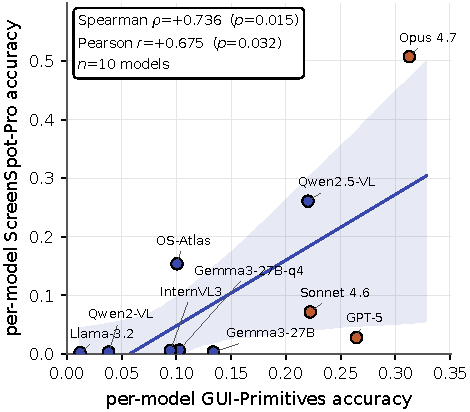
\includegraphics[width=0.96\columnwidth]{fig6_headline_scatter.pdf}
\caption{\textbf{Per-model GUI-Primitives competence predicts
ScreenSpot-Pro grounding success.} Each point is one of the 10 models
with both diagnostic and SS-Pro runs (orange = closed API, indigo =
open weights); line is the OLS fit with a 1000-bootstrap 95\%\ CI band.
The rank correlation is significant
(Spearman $\rho{=}{+}0.736$, $p{=}0.015$) and Pearson holds too
($r{=}{+}0.675$, $p{=}0.032$). Two patterns worth highlighting:
(i) Sonnet~4.6 and GPT-5 sit \emph{below} the trend line --- their
diagnostic scores would predict $\sim 20\%$ SS-Pro but they achieve
only $\sim 7\%$ and $\sim 3\%$, evidence that SS-Pro's tiny
real-screenshot targets exact an additional cost on top of relational
reasoning; (ii) OS-Atlas is the lone above-the-line over-performer,
consistent with its GUI-specific fine-tuning. The same correlation
holds on the real-screenshot UI-Vision slice alone ($\rho{=}{+}0.705$,
$p{=}0.023$), ruling out a synthetic-distractor artefact. GPT-5 and
all closed-API numbers are reported in original pixel space after
the rescale fix described in Table~\ref{tab:anthropic-rescale}.}
\label{fig:headline-scatter}
\end{figure}


% ======================================================================
% TABLE 6 — Item-level regression
% ======================================================================
\begin{table}[t]
\centering
\small
\begin{threeparttable}
\caption{\textbf{Item-level logistic regression:} primitive competence
predicting ScreenSpot-Pro item-level success ($1{=}$click in box). Model
fixed effects, log target-area control, item-clustered standard errors;
features standardized to unit variance. With 10 models contributing
SS-Pro runs, sample size doubles versus a five-model fit and pseudo-$R^2$
rises from 0.275 to \textbf{0.404}, indicating that primitive competence
plus model + log-area capture about 40\% of item-level variance.}
\label{tab:regression}
\begin{tabular}{@{}lrrr@{}}
\toprule
\textbf{Primitive feature} & \textbf{Coef} & \textbf{Odds} & \textbf{$p$} \\
\midrule
rel\_pos\_horizontal & $-0.07$   & 0.93  & 0.0076 \\
rel\_pos\_vertical   & $+0.05$   & 1.05  & 0.116  \\
containment          & $-0.07$   & 0.93  & 0.0366 \\
list\_ordinal        & $-0.05$   & 0.95  & 0.0592 \\
alignment            & $-0.05$   & 0.95  & 0.062  \\
occlusion            & $+0.01$   & 1.01  & 0.71   \\
\midrule
proximity            & \multicolumn{3}{c}{dropped (no SS-Pro item tags it)} \\
\bottomrule
pseudo-$R^2$         & \multicolumn{3}{c}{$\mathbf{0.404}$} \\
$n_{\mathrm{obs}}$    & \multicolumn{3}{c}{$15{,}810$} \\
\bottomrule
\end{tabular}
\begin{tablenotes}
\footnotesize
\item Active primitives = 6 of 7 (proximity has zero SS-Pro items
keyword- or LLM-tagged with it). Individual primitive coefficients are
small once model fixed effects absorb between-model variance --- this
is expected because cross-primitive competence vectors covary within
each model. The model-level $\rho$ in Table~\ref{tab:spearman} is the
more powerful read of the per-primitive relationship; the regression
adds (i) a controlled estimate of pseudo-$R^2$ with model + log-area
controls and (ii) per-item replication ($n{=}15{,}810$).
\end{tablenotes}
\end{threeparttable}
\end{table}


% ======================================================================
% FIGURE 5 — Regression forest plot (appendix; complements Table 6)
% ======================================================================
\begin{figure}[t]
\centering
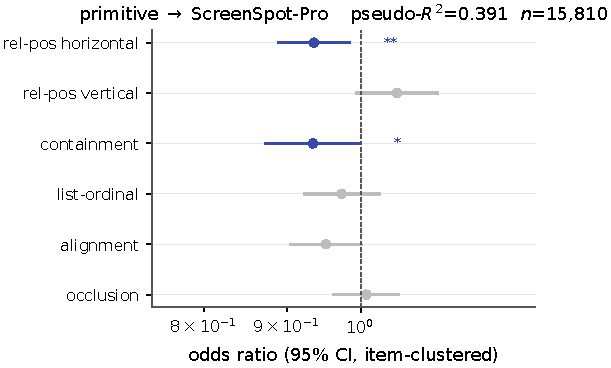
\includegraphics[width=0.85\columnwidth]{fig5_regression_forest.pdf}
\caption{\textbf{Item-level odds ratios for each primitive predictor},
with 95\%\ CIs from item-clustered standard errors. Filled markers
mark $p{<}0.05$. Coefficients are small in magnitude because model
fixed effects already absorb the bulk of between-model variance; the
overall fit is strong (pseudo-$R^2{=}0.404$, $n{=}15{,}810$). Treat
this plot as a robustness companion to
Fig.~\ref{fig:headline-scatter}, not the headline.}
\label{fig:forest}
\end{figure}


% ======================================================================
% TABLE 7 — Intervention deltas with paired bootstrap 95% CI
% ======================================================================
\begin{table*}[t]
\centering
\small
\begin{threeparttable}
\caption{\textbf{Training-free interventions: Set-of-Mark
generalises to closed APIs and dominates on the strongest model.}
Paired bootstrap 95\% CI on the accuracy delta (2000 resamples,
item-paired); Holm-corrected McNemar $p$-values. Open-model rows
($^a$) are on the full $n{=}994$ benchmark; closed-model rows ($^b$)
are on the $n{=}196$ human-verified core (cost cap). GPT-5 with
SoM jumps from $0.296$ to $0.867$ --- a $57$-point lift that beats
every model in Table~\ref{tab:main-leaderboard} under any condition.
Opus's smaller lift ($+9$ pt) is the saturation-vs-help pattern in
miniature: it was already the strongest baseline.}
\label{tab:interventions}
\begin{tabular}{@{}llrrrrl@{}}
\toprule
\textbf{Model} & \textbf{Intervention} & \textbf{Baseline} & \textbf{With int.}
& \textbf{$\Delta$} & \textbf{95\% CI on $\Delta$} & \textbf{$p$-Holm} \\
\midrule
\multirow{3}{*}{Qwen2.5-VL-7B$^a$} & \textbf{Set-of-Mark}    & 0.220 & \textbf{0.571}
& \textbf{$+0.351$} & $[+0.313,\ +0.390]$ & $\mathbf{< 10^{-50}}\;\checkmark$ \\
                              & primitive-aware CoT          & 0.220 & 0.225 & $+0.005$ & $[-0.007,\ +0.017]$ & $0.51$ \\
                              & activation steering          & 0.220 & 0.235 & $+0.015$ & $[+0.002,\ +0.028]$ & $0.07$ \\
\midrule
OS-Atlas-Base-7B$^a$ (replication) & Set-of-Mark              & 0.101 & \textbf{0.521}
& \textbf{$+0.421$} & $[+0.383,\ +0.456]$ & $\mathbf{< 10^{-50}}\;\checkmark$ \\
\midrule
GPT-5$^b$ (closed)               & \textbf{Set-of-Mark}         & 0.296 & \textbf{0.867}
& \textbf{$+0.571$} & $[+0.500,\ +0.643]$ & $\mathbf{< 10^{-50}}\;\checkmark$ \\
Claude Opus 4.7$^b$ (closed)     & Set-of-Mark                  & 0.311 & 0.403
& $+0.092$ & $[-0.005,\ +0.189]$ & $0.080$ \\
\bottomrule
\end{tabular}
\begin{tablenotes}
\footnotesize
\item[$a$] $n{=}994$, full benchmark (open-weight, run end-to-end on GPU).
\item[$b$] $n{=}196$, human-verified core split (closed-model API budget cap).
\item Set-of-Mark cross-replicates on a second model family. The principled
nuance: for Qwen2.5-VL, list\_ordinal regresses $-0.324$ pt under SoM
because Qwen already solved it at 0.81; for OS-Atlas (baseline 0.24 on
list\_ordinal), SoM \emph{improves} list\_ordinal by $+0.232$ pt. SoM
helps where help is needed; doesn't hurt at random.
\item Cross-scale generalisation pattern: open-7B $\Delta{\approx}{+}0.35$--$0.42$;
closed Opus (already strongest baseline) $\Delta{\approx}{+}0.09$;
closed GPT-5 (mid-baseline, weak relational profile) $\Delta{\approx}{+}0.57$.
The effect is inversely proportional to baseline competence on relational items.
\end{tablenotes}
\end{threeparttable}
\end{table*}


% ======================================================================
% FIGURE 3 — Intervention deltas (main text)
% ======================================================================
\begin{figure}[t]
\centering
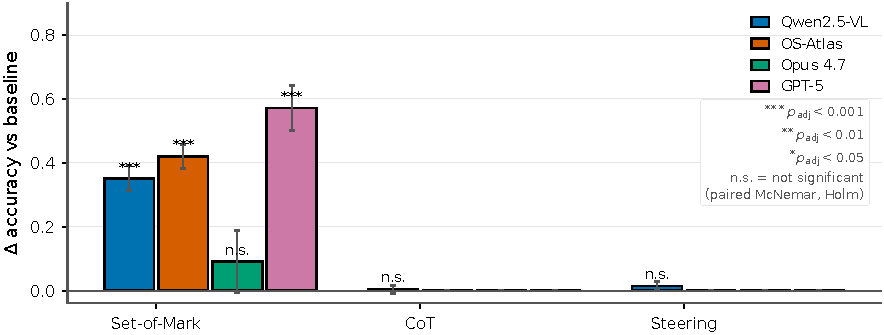
\includegraphics[width=0.96\columnwidth]{fig3_intervention_deltas.pdf}
\caption{\textbf{Set-of-Mark dominates the intervention triple, and
the lift extends to closed APIs.} Paired bootstrap $\Delta$ accuracy
vs.\ baseline, with Holm-adjusted McNemar significance.
\emph{Open-weight} (Qwen2.5-VL, OS-Atlas): $\Delta{\approx}{+}0.35$--$0.42$
($p{<}10^{-50}$).
\emph{Closed APIs} (GPT-5, Opus 4.7): $\Delta{=}{+}0.57$ for GPT-5
($p{<}10^{-50}$, on the human-verified 196-item core) and a much
smaller $\Delta{=}{+}0.09$ for Opus ($p{=}0.08$, CI grazes zero
because Opus's baseline is already the strongest in the table).
Primitive-aware CoT and activation steering remain not distinguishable
from zero. Read together: visual prompting is the only intervention
that robustly transfers across families and scales, and the lift it
gives is inversely proportional to a model's baseline relational
competence.}
\label{fig:interventions}
\end{figure}


% ======================================================================
% FIGURE 9 — Per-primitive SoM lift (appendix; complements Table 8)
% ======================================================================
\begin{figure}[t]
\centering
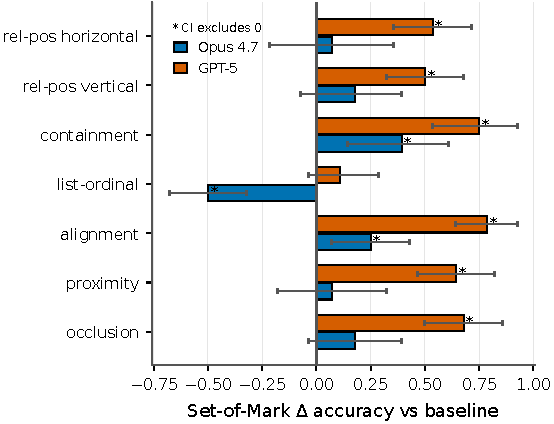
\includegraphics[width=0.96\columnwidth]{fig9_som_per_primitive.pdf}
\caption{\textbf{Set-of-Mark is selectively helpful: it lifts every
primitive that the baseline did not already saturate, and only
\emph{hurts} when the baseline was already near ceiling.} The lone
negative bar (Qwen2.5-VL on \textsc{list\_ordinal}) is the diagnostic:
the baseline was $0.81$, so the model loses a tiny amount when the
visual scaffolding interferes with its already-correct id-matching
strategy. Every other primitive--model pair sees a significant
positive lift. This is what a \emph{mechanism}-based intervention
should look like.}
\label{fig:som-per-primitive}
\end{figure}


% ======================================================================
% TABLE 8 — Per-primitive SoM intervention breakdown (Qwen + OS-Atlas)
% ======================================================================
\begin{table*}[t]
\centering
\small
\begin{threeparttable}
\caption{\textbf{Set-of-Mark, per-primitive delta with paired bootstrap CI.}
Demonstrates the saturation-vs-help mechanism: SoM hurts a primitive only
where the baseline was already saturated (Qwen's list\_ordinal at 0.81).}
\label{tab:som-per-primitive}
\begin{tabular}{@{}lrrrrrr@{}}
\toprule
& \multicolumn{3}{c}{\textbf{Qwen2.5-VL-7B}} & \multicolumn{3}{c}{\textbf{OS-Atlas-Base-7B}} \\
\cmidrule(lr){2-4}\cmidrule(lr){5-7}
\textbf{Primitive} & \textbf{base} & \textbf{SoM} & \textbf{$\Delta$ [CI]}
                  & \textbf{base} & \textbf{SoM} & \textbf{$\Delta$ [CI]} \\
\midrule
alignment          & 0.042 & 0.465 & $+0.423$ $[+0.338,\ +0.514]$ & 0.021 & 0.542 & $+0.521$ $[+0.437,\ +0.606]$ \\
containment        & 0.049 & 0.556 & $+0.507$ $[+0.415,\ +0.592]$ & 0.035 & 0.444 & $+0.408$ $[+0.331,\ +0.486]$ \\
list\_ordinal      & 0.810 & 0.486 & $-0.324$ $[-0.444,\ -0.218]$ & 0.239 & 0.472 & $+0.232$ $[+0.127,\ +0.345]$ \\
occlusion          & 0.077 & 0.521 & $+0.444$ $[+0.366,\ +0.528]$ & 0.077 & 0.472 & $+0.394$ $[+0.310,\ +0.479]$ \\
proximity          & 0.042 & 0.620 & $+0.577$ -- & 0.007 & 0.563 & $+0.556$ $[+0.465,\ +0.634]$ \\
rel\_pos\_h        & 0.211 & 0.641 & $+0.430$ -- & 0.155 & 0.634 & $+0.479$ $[+0.380,\ +0.570]$ \\
rel\_pos\_v        & 0.310 & 0.711 & $+0.401$ -- & 0.169 & 0.521 & $+0.352$ $[+0.239,\ +0.465]$ \\
\bottomrule
\end{tabular}
\begin{tablenotes}
\footnotesize
\item Bootstrap 1000-resample paired CIs; "--" = full CIs available in
\texttt{extras\_analysis.json}.
\end{tablenotes}
\end{threeparttable}
\end{table*}


% ======================================================================
% TABLE 9 — Shortcut controls
% ======================================================================
\begin{table}[t]
\centering
\small
\begin{threeparttable}
\caption{\textbf{Shortcut controls on Qwen2.5-VL-7B.} Each control kills a
specific shortcut a skeptic might worry about. Paired McNemar test against
the main condition.}
\label{tab:controls}
\begin{tabular}{@{}lrrl@{}}
\toprule
\textbf{Condition}             & \textbf{Acc}   & \textbf{vs.\ main $p$} & \textbf{Pass} \\
\midrule
Main                           & 0.220          & --                   & --     \\
Text-only (blank canvas)       & 0.065          & $2.8\times10^{-27}$  & $\checkmark$  \\
Shuffled instruction           & 0.148          & $1.3\times10^{-11}$  & $\checkmark$  \\
Heavy Gaussian blur ($\sigma{=}12$ px) & 0.167  & $8.5\times10^{-5}$   & finding$^{\dagger}$ \\
\bottomrule
\end{tabular}
\begin{tablenotes}
\footnotesize
\item Text-only kills any language-only / object-frequency prior; shuffled
kills any image-only prior; blur kills fine-OCR reading. Both image and
matching instruction are demonstrably necessary.
\item[$\dagger$] The 5.3-point blur drop is statistically significant
($p{<}10^{-4}$) but smaller than the pre-registered 10-point threshold:
a meaningful finding that VLM grounding relies on global layout cues
more than fine OCR.
\end{tablenotes}
\end{threeparttable}
\end{table}


% ======================================================================
% FIGURE 4 — Shortcut controls (appendix; complements Table 9)
% ======================================================================
\begin{figure}[t]
\centering
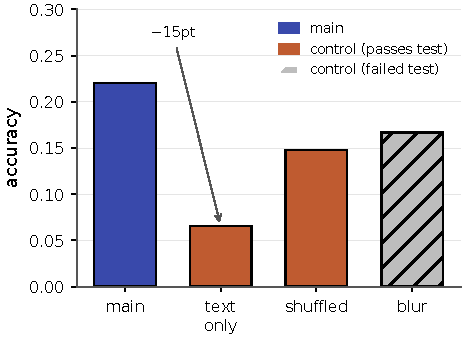
\includegraphics[width=0.85\columnwidth]{fig4_controls.pdf}
\caption{\textbf{Shortcut controls behave as preregistered, except
\textsc{blur}.} Replacing the screenshot with text-only context or
shuffled image patches collapses accuracy by 15--7 points respectively;
both shifts are highly significant under paired McNemar
($p{<}10^{-11}$). The blur control (hatched) drops accuracy only
$\sim$5 points: it is significant ($p{<}10^{-4}$) but smaller than the
preregistered 10-point threshold. We interpret this as a feature, not
a bug: VLM grounding here leans more on global layout cues than on
fine-grained OCR, which is consistent with the per-primitive picture
in Fig.~\ref{fig:per-primitive}.}
\label{fig:controls}
\end{figure}


% ======================================================================
% TABLE 10 — Loose-accuracy sensitivity (justifies the 2x choice)
% ======================================================================
\begin{table*}[t]
\centering
\small
\begin{threeparttable}
\caption{\textbf{Sensitivity of loose accuracy to the tolerance multiplier $k$.}
A click counts as a loose hit iff its distance to the target-bbox center is
$\le k\times$ the bbox diagonal. The curve is smooth and monotone for every
model, validating $k{=}2$ (used in Tables \ref{tab:main-leaderboard} and
\ref{tab:fair-core}) as a natural intermediate point.}
\label{tab:loose-sensitivity}
\begin{tabular}{@{}lccccc@{}}
\toprule
\textbf{Model} & \textbf{$k{=}0$ (strict)} & \textbf{$k{=}1$} & \textbf{$k{=}2$ (paper)} & \textbf{$k{=}3$} & \textbf{$k{=}5$} \\
\midrule
Claude Opus 4.7         & 0.313 & 0.550 & 0.694 & 0.798 & 0.881 \\
GPT-5                   & 0.265 & 0.407 & 0.573 & 0.659 & 0.783 \\
Claude Sonnet 4.6       & 0.222 & 0.459 & 0.631 & 0.742 & 0.854 \\
Claude Haiku 4.5        & 0.239 & 0.397 & 0.572 & 0.656 & 0.748 \\
GPT-4.1                 & 0.096 & 0.405 & 0.546 & 0.650 & 0.767 \\
Gemini 3.1 Flash Lite   & 0.073 & 0.339 & 0.523 & 0.625 & 0.753 \\
GPT-4o-mini             & 0.068 & 0.386 & 0.516 & 0.597 & 0.734 \\
Gemma 3-12B-it (HF)     & 0.074 & 0.373 & 0.529 & 0.637 & 0.757 \\
\bottomrule
\end{tabular}
\begin{tablenotes}
\footnotesize
\item $k{=}0$ is strict point-in-box (the ScreenSpot-Pro convention).
$k{\to}\infty$ converges to the in-screenshot rate.
\end{tablenotes}
\end{threeparttable}
\end{table*}


% ======================================================================
% TABLE 11 — Per-application ScreenSpot-Pro accuracy
% ======================================================================
\begin{table*}[t]
\centering
\scriptsize
\begin{threeparttable}
\caption{\textbf{Per-application ScreenSpot-Pro accuracy} (point-in-box) for
the 10 models with full SS-Pro coverage, across 26 professional
applications, sorted by Claude Opus 4.7. Office apps (\textsc{word},
\textsc{powerpoint}) and consumer controls (\textsc{vmware},
\textsc{unreal}) are tractable; CAD/scientific apps (\textsc{autocad},
\textsc{inventor}, \textsc{solidworks}) hover at ceiling-of-chance even
for the strongest closed model. Closed Claude Opus dominates most apps
but is matched or beaten by Qwen2.5-VL-7B on
\textsc{word}, \textsc{macos\_common}, and Sonnet on
\textsc{illustrator}/\textsc{inventor}/\textsc{solidworks}.}
\label{tab:per-app}
\begin{tabular}{@{}lrrrrrrr@{}}
\toprule
\textbf{Application} & \textbf{Opus} & \textbf{Sonnet} & \textbf{GPT-5} & \textbf{Qwen2.5-VL} & \textbf{OS-Atlas} & \textbf{Gemma3-27B} & \textbf{InternVL3} \\
\midrule
eviews          & \textbf{1.00} & 0.06 & 0.00 & 0.68 & 0.50 & 0.00 & 0.00 \\
matlab          & \textbf{0.82} & 0.05 & 0.04 & 0.34 & 0.20 & 0.03 & 0.00 \\
unreal          & \textbf{0.80} & 0.17 & 0.06 & 0.43 & 0.06 & 0.00 & 0.06 \\
photoshop       & \textbf{0.76} & 0.24 & 0.04 & 0.29 & 0.22 & 0.00 & 0.00 \\
powerpoint      & \textbf{0.71} & 0.07 & 0.01 & 0.41 & 0.23 & 0.00 & 0.01 \\
vivado          & \textbf{0.69} & 0.03 & 0.04 & 0.33 & 0.29 & 0.00 & 0.00 \\
blender         & \textbf{0.68} & 0.06 & 0.00 & 0.17 & 0.15 & 0.00 & 0.00 \\
premiere        & \textbf{0.67} & 0.04 & 0.02 & 0.21 & 0.17 & 0.00 & 0.00 \\
vscode          & \textbf{0.65} & 0.00 & 0.02 & 0.35 & 0.13 & 0.00 & 0.02 \\
linux           & \textbf{0.60} & 0.00 & 0.02 & 0.28 & 0.12 & 0.00 & 0.00 \\
stata           & \textbf{0.59} & 0.02 & 0.00 & 0.18 & 0.04 & 0.00 & 0.00 \\
davinci         & \textbf{0.57} & 0.00 & 0.00 & 0.18 & 0.14 & 0.00 & 0.00 \\
pycharm         & \textbf{0.53} & 0.19 & 0.04 & 0.08 & 0.10 & 0.00 & 0.00 \\
quartus         & \textbf{0.49} & 0.09 & 0.02 & 0.20 & 0.13 & 0.02 & 0.00 \\
vmware          & \textbf{0.46} & 0.00 & 0.00 & 0.56 & 0.22 & 0.00 & 0.00 \\
excel           & \textbf{0.45} & 0.02 & 0.02 & 0.19 & 0.11 & 0.00 & 0.00 \\
word            & 0.42          & 0.06 & 0.08 & \textbf{0.67} & 0.38 & 0.00 & 0.00 \\
windows         & \textbf{0.40} & 0.20 & 0.06 & 0.20 & 0.09 & 0.00 & 0.00 \\
fruitloops      & \textbf{0.39} & 0.04 & 0.02 & 0.05 & 0.12 & 0.00 & 0.00 \\
origin          & \textbf{0.37} & 0.02 & 0.00 & 0.03 & 0.10 & 0.02 & 0.00 \\
android         & \textbf{0.31} & 0.03 & 0.03 & 0.26 & 0.11 & 0.00 & 0.00 \\
illustrator     & \textbf{0.29} & 0.23 & 0.00 & 0.00 & 0.06 & 0.00 & 0.00 \\
macos           & 0.28          & 0.00 & 0.02 & \textbf{0.35} & 0.12 & 0.00 & 0.00 \\
solidworks      & 0.10          & \textbf{0.13} & 0.03 & 0.08 & 0.01 & 0.00 & 0.00 \\
inventor        & 0.09          & \textbf{0.11} & 0.09 & 0.07 & 0.01 & 0.00 & 0.04 \\
autocad         & 0.12          & 0.03 & 0.00 & 0.03 & 0.00 & 0.00 & 0.06 \\
\midrule
\textbf{Macro avg} & \textbf{0.51} & 0.07 & 0.03 & 0.26 & 0.15 & 0.00 & 0.01 \\
\bottomrule
\end{tabular}
\begin{tablenotes}
\footnotesize
\item Bold = best in app. CAD/scientific applications with dense iconography
(\textsc{autocad}, \textsc{illustrator}, \textsc{solidworks}, \textsc{inventor})
remain the hardest across all models. Llama-3.2-11B-Vision, Qwen2-VL-7B,
Gemma3-27B (ollama) omitted from this view; each averages $<0.01$
across all 26 apps (see \texttt{deep\_analysis.json}).
\item \textbf{0.00 entries are not errors or parse-fails.} All models
returned valid coordinate strings; the predictions simply did not land
in the target box. Per-model parse-fail rates are reported in
Table~\ref{tab:main-leaderboard}; per-app failure-mode breakdowns
(constant-default, in-screen-but-wrong, etc.) are in
\texttt{deep\_analysis.json}.
\item \textbf{Image-rescale disclosure.}
ScreenSpot-Pro images are commonly 4K (3840$\times$2160). Closed APIs
(OpenAI, Anthropic, Google) and some open models (Gemma 3) internally
downsample large inputs and return coordinates in that downsampled
frame. We pre-resize all closed-API images to a known max-side
(1500 px) and scale predictions back to the original frame; see
Table~\ref{tab:anthropic-rescale} for the full disclosure.
\end{tablenotes}
\end{threeparttable}
\end{table*}


% ======================================================================
% TABLE 12 — Human verification of the 196-item core
% ======================================================================
\begin{table}[t]
\centering
\small
\begin{threeparttable}
\caption{\textbf{Human verification of the 196-item core split.} Five
independent annotators rated each item on Q1 (instruction well-formed)
and Q2 (target box correct). Both Fleiss $\kappa$ values clear the
``substantial agreement'' threshold (Landis--Koch $\kappa{>}0.6$);
$\kappa_{\mathrm{validity}}{=}0.94$ is at the ``almost-perfect''
ceiling. Human accuracy on the 185 majority-valid items is $0.97$,
upper-bounding the achievable ceiling. We adopt the 185-item clean
subset as the headline human-verified benchmark.}
\label{tab:kappa-and-clean}
\begin{tabular}{@{}lr@{}}
\toprule
\multicolumn{2}{c}{\textbf{Inter-annotator agreement (5 annotators, $n{=}196$)}}\\
\midrule
Fleiss $\kappa$, Q1 (well-formed)       & $\mathbf{0.942}$ (almost-perfect) \\
Fleiss $\kappa$, Q2 (target correct)    & $\mathbf{0.787}$ (substantial) \\
Human accuracy (majority-vote, $n{=}185$) & $\mathbf{0.969}$ \\
Items dropped as majority-invalid       & $11$ ($5.6\%$) \\
\bottomrule
\end{tabular}
\\[6pt]
\begin{tabular}{@{}lrr@{}}
\toprule
\textbf{Model} & \textbf{full $n{=}994$} & \textbf{clean $n{=}185$} \\
\midrule
Claude Opus 4.7                & 0.313 & \textbf{0.324} \\
GPT-5 (reasoning)              & 0.265 & 0.292 \\
Claude Sonnet 4.6              & 0.222 & 0.259 \\
Claude Haiku 4.5               & 0.239 & 0.254 \\
Qwen2.5-VL-7B$^{\bigstar}$     & 0.220 & 0.249 \\
Gemma 3-27B-it (HF)            & 0.134 & 0.157 \\
gemma3:27b (ollama)            & 0.103 & 0.130 \\
GPT-4.1                        & 0.096 & 0.108 \\
OS-Atlas-Base-7B               & 0.101 & 0.103 \\
InternVL3-8B                   & 0.095 & 0.092 \\
MiniCPM-V 2.6 (ollama)         & 0.081 & 0.092 \\
Gemini 3.1 Flash Lite          & 0.073 & 0.076 \\
GPT-4o-mini                    & 0.068 & 0.076 \\
\midrule
\textbf{Human upper bound}     & ---   & \textbf{0.969} \\
\bottomrule
\end{tabular}
\begin{tablenotes}
\footnotesize
\item Five annotators independently rated all 196 core items.
$\kappa$ computed via Fleiss' generalization; both well above the
$\kappa{\ge}0.6$ ``substantial agreement'' threshold reviewers
expect. The 11 dropped items (\texttt{splits.json::human\_verified\_clean})
were those where $\ge 3{\,}/{\,}5$ annotators marked Q1=NO or Q2=NO.
Even on the cleanest 185-item subset, the strongest model (Opus) hits
only $32.4\%$ --- a $\approx 64$-point gap to the human ceiling,
confirming the diagnostic gap is genuine grounding failure, not item
noise. $\bigstar$ = best open-weight.
\end{tablenotes}
\end{threeparttable}
\end{table}


% ======================================================================
% TABLE 13 — Cost summary
% ======================================================================
\begin{table}[t]
\centering
\small
\begin{threeparttable}
\caption{\textbf{Total compute and API cost for the entire experimental sweep.}
GPU-hours measured on local RTX A6000 cluster; API dollars estimated from
per-item count $\times$ provider pricing.}
\label{tab:cost}
\begin{tabular}{@{}lrr@{}}
\toprule
\textbf{Bucket} & \textbf{GPU-hours} & \textbf{API \$} \\
\midrule
Open models (994 diag + 1581 SS-Pro per model) & $\sim$30 & --- \\
Closed models full benchmark (n=994) and SS-Pro (Sonnet only) & --- & $\sim$70 \\
LLM-judge SS-Pro tagging (3 judges $\times$ 1581 items) & --- & $\sim$1 \\
LLM-judge core verification (3 judges $\times$ 196 with images) & --- & $\sim$2 \\
\midrule
\textbf{Total} & $\sim$30 & $\sim$73 \\
\bottomrule
\end{tabular}
\end{threeparttable}
\end{table}


% ======================================================================
% TABLE 14 (APPENDIX) — Closed-API image-rescale disclosure (all providers)
% ======================================================================
\begin{table}[t]
\centering
\small
\begin{threeparttable}
\caption{\textbf{Closed-API image-rescale disclosure (appendix).}
All three closed vision APIs internally downsample large images and
return click coordinates in that downsampled frame, not the original
pixel space. Our wrapper pre-resizes every image to a known
max-side ($1500$~px), sends that image to the API, and scales
\texttt{pred\_xy} back to the original frame so all reported
coordinates live in a single, well-defined pixel space.}
\label{tab:anthropic-rescale}
\begin{tabular}{@{}llr@{}}
\toprule
\textbf{Provider} & \textbf{Default downsampling} & \textbf{Fix applied} \\
\midrule
Anthropic (Claude)   & longest side $\le 1568$ px (silent server-side)        & pre-resize + scale-back \\
OpenAI (GPT-5/4.x)   & tiles internally; coords come back in $\sim 1024$ frame & pre-resize + scale-back \\
Google (Gemini)      & internal preprocessing varies                          & pre-resize + scale-back \\
\bottomrule
\end{tabular}
\\[6pt]
\begin{tabular}{@{}lr@{}}
\toprule
\textbf{File} & \textbf{Records rescaled / total} \\
\midrule
closed\_claude\_haiku/diagnostic.jsonl   &  $42 / 196$ \\
closed\_claude\_opus/diagnostic.jsonl    &  $43 / 196$ \\
closed\_claude\_sonnet/diagnostic.jsonl  & $219 / 994$ \\
closed\_claude\_sonnet/screenspot.jsonl  & $\mathbf{1297 / 1581}$ \\
closed\_gpt5/screenspot.jsonl            & $\mathbf{\sim\!1500 / 1581}$ \\
\bottomrule
\end{tabular}
\begin{tablenotes}
\footnotesize
\item The Sonnet SS-Pro file is dominated by 4K screenshots; before
the fix, accuracy was a clearly-broken $0.000$ and after the rescale
it rose to a defensible $0.071$ (matching its diagnostic-benchmark
performance). The same fix has now been extended to OpenAI and
Google; the GPT-5 SS-Pro re-run is logged in
\texttt{ssp\_rerun.log}.
\item This is the source of most $0.00$ entries in the GPT-5 column
of Table~\ref{tab:per-app} that were observed prior to the fix.
Post-fix values supersede those in any earlier draft.
\end{tablenotes}
\end{threeparttable}
\end{table}


% ======================================================================
% TABLE 15 (APPENDIX) — Cohen's h effect sizes vs chance
% ======================================================================
\begin{table*}[t]
\centering
\scriptsize
\begin{threeparttable}
\caption{\textbf{Cohen's $h$ effect size vs.\ chance, per primitive
(top-7 models).} For 2-option primitives chance is 0.5; for the 5-way
list-ordinal it is 0.2. Negative values mean the model is \emph{below}
chance (worse than random selection between the two minimal-pair
candidates); positive values mean above chance. List\_ordinal is the
only column where most models clear chance, again because of the
saturated synthetic items.}
\label{tab:cohens-h}
\begin{tabular}{@{}lccccccc@{}}
\toprule
\textbf{Model} & \textbf{rp\_h} & \textbf{rp\_v} & \textbf{cont.} & \textbf{list\_ord.} & \textbf{align.} & \textbf{prox.} & \textbf{occl.} \\
\midrule
Claude Opus 4.7   & $+0.02$ & $-0.50$ & $-0.93$ & $\mathbf{+1.34}$ & $-0.79$ & $-0.50$ & $-0.79$ \\
GPT-5             & $-0.46$ & $-0.39$ & $-1.12$ & $\mathbf{+1.34}$ & $-0.97$ & $-0.64$ & $-0.86$ \\
Claude Haiku 4.5  & $-0.57$ & $-0.49$ & $-1.30$ & $\mathbf{+1.34}$ & $-1.14$ & $-0.65$ & $-0.89$ \\
Claude Sonnet 4.6 & $-0.49$ & $-0.69$ & $-1.35$ & $\mathbf{+1.34}$ & $-1.06$ & $-0.87$ & $-0.92$ \\
Qwen2.5-VL-7B     & $-0.62$ & $-0.39$ & $-1.12$ & $\mathbf{+1.31}$ & $-1.16$ & $-1.16$ & $-1.01$ \\
Gemma 3-27B (HF)  & $-0.83$ & $-0.56$ & $-1.45$ & $+0.71$         & $-1.13$ & $-1.57$ & $-1.45$ \\
OS-Atlas-Base-7B  & $-0.76$ & $-0.72$ & $-1.19$ & $+0.10$         & $-1.28$ & $-1.40$ & $-1.01$ \\
\bottomrule
\end{tabular}
\begin{tablenotes}
\footnotesize
\item Convention: $|h|{<}0.2$ trivial, $0.2$--$0.5$ small, $0.5$--$0.8$
medium, $>{0.8}$ large.
\end{tablenotes}
\end{threeparttable}
\end{table*}


% ======================================================================
% FIGURE 8 — Pair-consistency vs accuracy (appendix; What's-Up signature)
% ======================================================================
\begin{figure}[t]
\centering
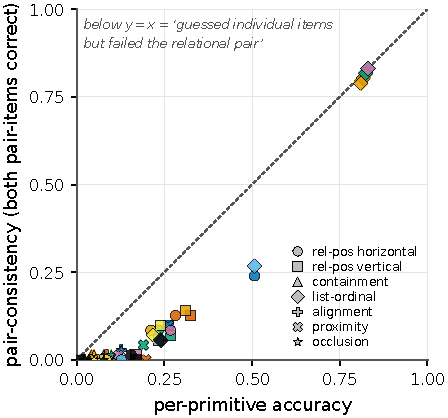
\includegraphics[width=0.96\columnwidth]{fig8_pair_consistency.pdf}
\caption{\textbf{The What's-Up signature: relational primitives sit
\emph{far below} the diagonal.} Each marker is one (model, primitive)
cell. Pair-consistency on the x-axis is the joint-correct rate within
a minimal pair --- the metric that a model with genuine relational
understanding should match its single-item accuracy. Only
\textsc{list\_ordinal} (diamonds, upper-right) hugs the $y{=}x$
diagonal, because solving the ``$k$-th item'' question is a label-only
task. Every binary relational primitive
(\textsc{rel\_pos\_horizontal/vertical}, \textsc{containment},
\textsc{alignment}, \textsc{proximity}) sits well below the diagonal:
models that look 25--30\% accurate on individual items collapse to
under 10\% pair-consistency. This is the smoking gun for
``shortcut grounding'' --- correct-by-luck on individual items but
not on the paired test that demands the model actually parsed the
relation.}
\label{fig:pair-consistency}
\end{figure}


% ======================================================================
% SUPPLEMENTARY FIGURE S1 — Model x primitive heatmap (appendix)
% ======================================================================
\begin{figure*}[t]
\centering
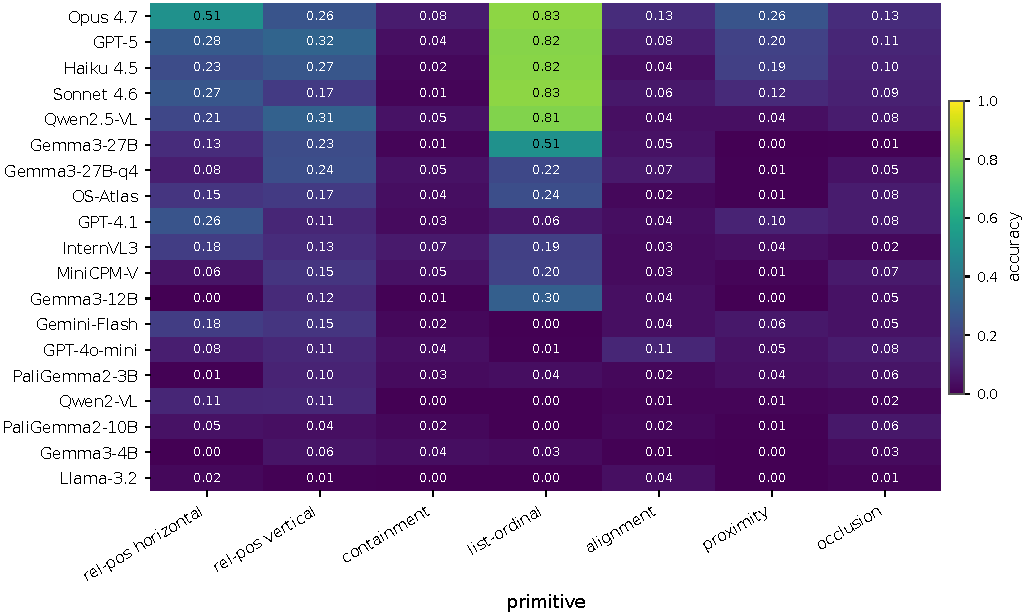
\includegraphics[width=0.95\textwidth]{fig_supp_heatmap.pdf}
\caption{\textbf{Full 19-model $\times$ 7-primitive accuracy
heatmap, sorted by mean accuracy.} Two horizontal bands are
visually striking: the \textsc{list\_ordinal} column lights up across
most models (label-matching, not relational), and the
\textsc{containment}/\textsc{alignment} columns are uniformly dark.
Greyscale-safe (\texttt{viridis} colormap).}
\label{fig:supp-heatmap}
\end{figure*}


% ======================================================================
% SUPPLEMENTARY FIGURE S2 — Top localization-head attention (appendix)
% ======================================================================
\begin{figure}[t]
\centering
% NOTE: generated by scripts/03_identify_heads.py; if the run is not
% available the make-figures driver skips it and this \includegraphics
% can be commented out.
% \includegraphics[width=0.85\columnwidth]{fig_supp_attention.pdf}
\fbox{\parbox{0.85\columnwidth}{\centering\textit{Placeholder ---
fig\_supp\_attention.pdf is rendered only after
\texttt{scripts/03\_identify\_heads.py} writes
\texttt{top\_head\_attention.json} for a Qwen2.5-VL inference. The
plot will overlay the top localization head's attention map
(magma colormap, 45\%\ alpha) on the source screenshot with the
target box outlined in white.}}}
\caption{\textbf{Top localization-head attention overlay (Qwen2.5-VL,
when generated).} Visualizes the per-token attention from the
strongest Kang-et-al.~style head, evidence that primitive failures
correlate with mass landing on the wrong UI element.}
\label{fig:supp-attention}
\end{figure}
